%CLASSE DOCUMENTO - LINGUA E DIMENSIONE FONT
\documentclass[corpo=11pt,english,numerazioneromana]{toptesi}

%%%%%%%%%%%%%%%%%%%%%%%%%%%%%%%%%%%%%%%%%%%%%%%%%%%%%%%%%%%%%%

% INCLUSIONE PACCHETTI
\usepackage[classica]{topfront}
\usepackage[utf8]{inputenc} %utf8
\usepackage[english]{babel}
\usepackage[T1]{fontenc}
\usepackage{blindtext}
\usepackage{graphicx,wrapfig}
\usepackage{booktabs}
\usepackage{lmodern}
\usepackage{varioref}
\usepackage{url}
\usepackage{array}
\usepackage{paralist}{\obeyspaces\global\let =\space}
\usepackage{verbatim}
\usepackage{subfig}
\usepackage{tabularx}
\usepackage{amsmath}
\usepackage{accents}
\usepackage{slashed}
\usepackage{amsfonts}
\usepackage{float}
\usepackage{amssymb}
\usepackage{multicol}
\usepackage{multirow}
\usepackage{listings}
\usepackage[pass]{geometry}
\usepackage[figuresright]{rotating}
\usepackage{algorithm}
\usepackage{algpseudocode}
\usepackage{amsmath}
\usepackage{physics}
\usepackage{bbold}
\usepackage[babel]{csquotes}
\usepackage{hyperref}
\usepackage{braket}
\usepackage{mathtools}
\usepackage{subfig}
\usepackage{setspace}
\graphicspath{ {images/} }
\usepackage[sorting=none,style=numeric-comp,backend=biber]{biblatex}
\usepackage{tikz}
\usepackage{mathdots}
\usepackage{yhmath}
\usepackage{cancel}
\usepackage{color}
\usepackage{siunitx}
\usepackage{array}
\usepackage{multirow}
\usepackage{amssymb}
\usepackage{gensymb}
\usepackage{tabularx}
\usepackage{extarrows}
\usepackage{booktabs}
\usetikzlibrary{fadings}
\usetikzlibrary{patterns}
\usetikzlibrary{shadows.blur}
\usetikzlibrary{shapes}

 \DeclareUnicodeCharacter{202F}{FIX ME!!!!}

%%%%%%%%%%%%%%%%%%%%%%%%%%%%%%%%%%%%%%%%%%%%%%%%%%%%%%%%%%%%%%%

% CONFIGURAZIONE LINK E RIFERIMENTI
\hypersetup{%
    pdfpagemode={UseOutlines},
    bookmarksopen,
    pdfstartview={FitH},
    colorlinks,
    linkcolor={black}, %COLORE DEI RIFERIMENTI AL TESTO
    citecolor={blue}, %COLORE DEI RIFERIMENTI ALLE CITAZIONI
    urlcolor={blue} %COLORI DEGLI URL
}

%%%%%%%%%%%%%%%%%%%%%%%%%%%%%%%%%%%%%%%%%%%%%%%%%%%%%%%%%%%%%%%

% CONFIGURAZIONE LISTATI/CODICE - CANCELLARE SE NON NECESSARIO
% PYTHON - BIANCO E NERO
\lstset{%
	captionpos=b,
	language=Python,
	basicstyle =\small\ttfamily,
	keywordstyle=\color{black}\bfseries,
	breaklines=true,
	breakatwhitespace=true,
	frame=lines,
	numbers=left,
	numberstyle=\footnotesize,
}

%%%%%%%%%%%%%%%%%%%%%%%%%%%%%%%%%%%%%%%%%%%%%%%%%%%%%%%%%%%%%%%

% FRENCHSPACING ABILITATO - CANCELLARE PER SPAZIATURA ALL'INGLESE
\frenchspacing

%%%%%%%%%%%%%%%%%%%%%%%%%%%%%%%%%%%%%%%%%%%%%%%%%%%%%%%%%%%%%%%

%DEFINIZIONE SEZIONI IN NUMERAZIONE ROMANA
%ELENCO DEI LISTATI/CODICI
\makeatletter
\newcommand\listofcodes{%
 \iffrontmatter\else\frontmattertrue\fi
 \if@openright\cleardoublepage\else\clearpage\fi
 % change the meaning of \chapter in a group
 \begingroup\def\chapter##1{\@schapter}
 \phantomsection % for the hyperlink
 \addcontentsline{toc}{chapter}{Listings}
 \lstlistoflistings 
 \endgroup
} 
\makeatother

%%%%%%%%%%%%%%%%%%%%%%%%%%%%%%%%%%%%%%%%%%%%%%%%%%%%%%%%%%%%%%%

% INFORMAZIONI PDF - PERSONALIZZARE
\pdfinfo{%
  /Title    (Factorization of the fermionic determinant in Lattice Field Theories)
  /Author   (Luca Virzì)
  /Subject  (Proposal for an alternive procedure applied to the Schwinger Model)
  /Keywords (Lattice lat-hep)
}

%%%%%%%%%%%%%%%%%%%%%%%%%%%%%%%%%%%%%%%%%%%%%%%%%%%%%%%%%%%%%%%

% LISTA DEI CAPITOLI DA INCLUDERE - PERSONALIZZARE
\includeonly{%
chap_intro, %
chap_schwinger, %
chap_obs,%
chap_fact,%
chap_newfact,
conclusion,
app_a,%
app_b,%
app_wdop,%
app_lu,
app_approx,
}

% FILE DI BIBLIOGRAFIA
\addbibresource{bibliography.bib}

%%%%%%%%%%%%%%%%%%%%%%%%%%%%%%%%%%%%%%%%%%%%%%%%%%%%%%%%%%%%%%%
% INIZIO DOCUMENTO
\begin{document}
\english

%%%%%%%%%%%%%%%%%%%%%%%%%%%%%%%%%%%%%%%%%%%%%%%%%%%%%%%%%%%%%%%


% FRONTESPIZIO - PERSONALIZZARE
% ELIMINATE LE VOCI CHE NON VI SERVONO

% UNIVERSITA - NOME
\ateneo{Università degli Studi Milano-Bicocca}

% FACOLTA - DICITURA
\FacoltaDi{Dipartimento di Fisica "Giuseppe Occhialini"}

% CORSO DI LAUREA - DICITURA (MANTENERE LO SPAZIO)
\CorsoDiLaureaIn{Corso di Laurea Magistrale in}
% CORSO DI LAUREA - NOME
\corsodilaurea{Fisica}

% LOGO UNIVERSITA
\logosede{logo-bicocca.pdf}

% TIPOLOGIA TESI
\TesiDiLaurea{Tesi di Laurea Magistrale}

% TITOLO
\titolo{Factorization of the fermionic determinant in Lattice Field Theories}

% SOTTOTITOLO
\sottotitolo{Proposal for an alternative procedure applied to the Schwinger Model}

% RELATORE/I - DICITURA
\AdvisorName{Relatore:}
% RELATORE - PROF. NOME E COGNOME
\relatore{Prof.\ Michele Pepe}
% RELATORE AGGIUNTIVO - PROF NOME E COGNOME
% SE SI HA SOLO UN RELATORE ELIMINARE E CAMBIARE Advisors in Advisor
\secondorelatore{Prof.\ Leonardo Giusti}

% CANDIDATO - DICITURA (MANTENERE I DUE PUNTI)
\CandidateName{Candidato:}
% SECONDO CANDIDATO - ELIMINARE O DECOMMENTARE
%secondocandidato{Bombo de Bombis}

% CANDIDATO - NOME E COGNOME
\candidato{Luca Virzì \\ Matricola: 850345}


% DATA - MESE ANNO
\sedutadilaurea{Marzo 2023 - A.A. 2021/22}

\frontespizio


%%%%%%%%%%%%%%%%%%%%%%%%%%%%%%%%%%%%%%%%%%%%%%%%%%%%%%%%%%%%%%%

%INTERLINEA - DEFAULT 1 - NON ESAGERATE, NON SUPERATE MAI 1.3 ;)
%\interlinea{1.2}

%%%%%%%%%%%%%%%%%%%%%%%%%%%%%%%%%%%%%%%%%%%%%%%%%%%%%%%%%%%%%%%



% CITAZIONE - PERSONALIZZARE
% VSPACE - PROPORZIONE USATA PER CENTRATURA VERTICALE DEL TESTO
% FLUSHRIGHT - ALLINEAMENTO ORIZZONTALE A DESTRA
\vspace*{\stretch{1}}
\begin{flushright}
\noindent
%To anyone who struggled in this system based on competition \\
%you will not go unheard
%e intanto tutti fanno strada \\
%stando fermi al posto loro
%\vspace{5 mm}
%\\ Giallorenzo
%\textit{Niccolò Contessa}
\end{flushright}
\vspace*{\stretch{6}}
\cleardoublepage



% ABSTRACT - PERSONALIZZARE
\sommario
The definition of quantum field theories on lattice is the only approach that allows us to explore their non-perturbative features in a formal way from first principles. This possibility becomes fundamental for instance for Quantum Chromodynamics (QCD), the quantum field theory which describes strong interactions, as it is characterised by asymptotic freedom. Namely, its coupling constant $\alpha_S$ becomes larger at smaller energy scales, making it impossible to study the theory perturbatively in this regime. The non-perturbative definition of QCD is indeed given by the continuum limit, at infinite volume, of the theory regolarized on lattice (Lattice QCD, LQCD).
\\ In the last decades the interest towards lattice field theories arose alongside a simultaneous exploit of our computational and numerical capabilities: if it is true that computers engineering knew an extraordinary progress in this time span, it is also undeniable that the state of art of computational Physics fondly relied on the design of better algorithms for the implementation of such theories.
\\ Monte Carlo algorithms consolidated as the most solid technique for the simulation of lattice field theories, in particular its variant called \textit{Hybrid Monte Carlo} (HMC), where the time evolution is deterministic and obeys the dynamics coming from the equations of motion of the system. 
\\ If Monte Carlo algorithms have been widely used for the implementation of pure gauge theories, numerical limits rise up when dynamical fermions come into the game, and one of the fondest challenges in this research branch consists in how to overcome those limits. The implementation of dynamical quarks indeed results in an additive term in the effective bosonic action of the system, the \textit{fermionic determinant}, which depends on gauge fields defined across the whole lattice and is consequently highly non-local.
\\ The worst consequence of this non-locality consists in the so-called \textit{exponential problem}, namely most hadronic correlation functions suffer from an exponential deterioration of the signal-to-noise ratio. This in turn implies that, in order to reach an adequate fixed statistical precision, the required computational costs grow exponentially, making simulations unfeasible in reasonable times for observables at great distances. 
\\ Recently in literature it was proposed that a possible way to tackle down this problem consists in the factorization of the fermionic determinant, which alongside the factorization of fermionic observables led to the first \textit{multi-level algorithms} for theories with dynamical quarks. The main ingredient of this procedure is the domain decomposition of the lattice into sub-lattices with independent dynamics, where the action can be written as a local functional of the block fields. More specificly, the lattice gets decomposed in overlapping blocks, so that the contributions to the correlation function coming from non-local terms are suppressed exponentially when the thickness of the overlapping region is increased. In this way, the exponential problem reduces to a polynomial one. 
\\ In this work we present an alternative procedure for the factorization of the quark determinant with respect to the one currently present in literature, where the decomposition in overlapping domains is substituted by a complete block-separation of the system dynamics.
\\ Once that also the factorization of fermionic observables will be formalized, we will compare the numerical effectiveness of this new algorithm, and since the computational costs required to perform a test in the framework of Lattice QCD would be exaggerated for our goal, the first verification will be carried on on a simpler system, namely the Schwinger Model (QED$_2$), which shares some computational features with LQCD.
\\ Given this consideration, this work started with the design of an HMC algorithm for the Standard Schwinger Model from scratches, where standard means that domain decomposition was not introduced. After a discussion of the equations of motions which drive the system dynamics, we present some numerical tests on the algorithmic efficiency of our code. Next we focus on the effectiveness of some stochastic estimators for fermionic observables, namely \textit{noise vectors}, whose implementation is crucial in more demanding simulations. Consequently we proceed with the computation of the correlation functions needed for the inspection of the low-lying spectrum of the theory, given by iso-triplet and iso-singlet states (in analogy with QCD$_4$), and in particular we focus on its behaviour towards the chiral limit.
\\ These results will be useful to test the efficiency of the algorithm in which the new factorization procedure will be implemented, whose realization represents our next goal. Finally, in order to support the theoretical validity of our proposal, we present the results of a numerical test for the factorization procedure conducted on a gauge configuration extrapolated from the aforementioned code.
%Abstract, pleased to meet you. Ah, it's not funny anymore.

%%%%%%%%%%%%%%%%%%%%%%%%%%%%%%%%%%%%%%%%%%%%%%%%%%%%%%%%%%%%%%%

% INDICI - ELIMINARE GLI INDICI NON NECESSARI

% INDICE GENERALE
\tableofcontents

% INDICE DELLE FIGURE
\listoffigures

% INDICE DELLE TABELLE
\listoftables

%%%%%%%%%%%%%%%%%%%%%%%%%%%%%%%%%%%%%%%%%%%%%%%%%%%%%%%%%%%%%%%

\mainmatter

% INCLUSIONE FILE CAPITOLI - PERSONALIZZARE - TENERE COERENTE CON LISTA IN ALTO
\chapter{Lattice Gauge Theories}
\label{chap:intro}
In this chapter we will explore the theoretical framework we work within, essentially the fundamentals of Lattice Gauge Theories. Our understanding of Nature and its fundamental forces is best expressed through Quantum Field Theories (QFT), and in particular we will rely on the Path Integral formalism. The definition of Lattice Gauge Theories comes from the necessity to write the path integral of such theories in a completely non-perturbative fashion, hence we will see how to define their building blocks and how they tangle with computational physics, using the Schwinger Model as a reference.
\\ The Schwinger Model \cite{Schwinger:1962tp} consists of a two-dimensional realization of Quantum Electrodynamics (QED$_2$), hence a quantum field theory with U(1) gauge symmetry, embedded with two mass-degenerate dynamical quarks. This model has been the subject of many extensive studies throughout the last decades, as it shares interesting features with more realistic field theories, such as Quantum Chromodynamics (QCD). In the Schwinger Model one can observe quarks confinement, chiral symmetry breaking, the formation of a fermionic condensate and of a non-trivial topological $\theta-$vacuum \cite{COLEMAN1975267, COLEMAN1976239}, hence it can be used as a toy-model to test new computational methods, with cheaper computational costs.
\\ Before moving on to the case-study of this thesis, it is useful to recall some basic principles about Lattice Gauge Theories, in particular the definition of a U(1) Abelian Gauge theory on lattice and the implementation of dynamical fermions within it.

\section{QED: Continuum Formulation}
In this section we will briefly review how to derive the QED gauge-invariant action in the continuum formulation, before moving on to the lattice formulation. For a more complete description, it is convenient to check Quantum Field Theory books, such as \cite{Peskin:1995ev, Rothe:1992nt}.
\\ Quantum Electrodynamics can be described in terms of a quantum field theory characterized by a U(1) local symmetry, hence an abelian and continuous symmetry group. 
\\ The classic gauge-invariant action of the photon field $A_\mu(x)$ is given by:
\begin{equation}\label{S_G}
    S_G\,[A_\mu] = - \frac{1}{4} \int d^4x F_{\mu \nu}(x) F^{\mu\nu}(x)
\end{equation}
where $F_{\mu \nu} (x) = \partial_\mu A_\nu(x) - \partial_\nu A_\mu(x)$ is the gauge invariant field strength tensor, and $x \equiv x^\mu = (x^0, x^1, x^2, x^3)$ is a space-time point. The action $S_G$ is invariant under local transformations:
\begin{equation}
    A_\mu(x) \to A_\mu'(x) = A_\mu(x) + \partial_\mu g(x)
\end{equation}
where $g(x) = e^{i\Lambda(x)}$ is an element of the abelian U(1) group.
\\ Consider now the action of the free Dirac-field $\psi(x)$:
\begin{equation}
    S_F \, [\psi, \Bar{\psi}] = \int d^4 x \, \Bar{\psi}(x) \left(i \gamma^{\mu} \partial_\mu - m \right) \psi(x)
\end{equation}
where $\gamma_\mu$ are a set of $4 \times 4$ matrices which satisfy the Clifford algebra $\{\gamma^\mu, \gamma^\nu\} = 2 \eta^{\mu\nu}$, and $m$ is the mass parameter associated to the field $\psi$.
\\ The action $S_F$ is invariant under global U(1) transformations:
\begin{equation}\label{u(1) global}
    \begin{split}
        \psi (x) \to & \, \psi'(x) = e^{-iq\theta}\psi(x) \\
        \Bar{\psi} (x) \to & \, \Bar{\psi'}(x) = e^{iq\theta}\Bar{\psi}(x) \\
    \end{split}
\end{equation}
where $q$ is a label for the one-dimensional representations of the group, and coincides with the charge of the field $\psi$. For a collection of fields $\psi_i$, we could use independent transformations of the form (\ref{u(1) global}), leading to an action which is invariant under several copies of U(1). Nevertheless, we are interested in a common U(1) subgroup of these copies, such that each field $\psi_i$ transforms with the same group transformation $e^{iq_i\theta}$, but accordingly to different representations labelled by $q_i$.
\\ We now want to promote this global invariance of the Dirac equation to a local one, such that it coincides with the local U(1) invariance of the photon field. Consequently the QED action $S_{QED}$ will have a U(1) gauge symmetry, where fermions transform under unitary representations of U(1) labelled by their electric charge $q$. This can be achieved by means of the so called \textit{minimal transformation}, i.e. we replace the ordinary four-derivative $\partial_\mu$ with the covariant derivative $D_\mu$, defined by:
\begin{equation}
    D_\mu = \partial_\mu + iq A_\mu \hspace{10mm} \slashed{D} = i\gamma^\mu D_\mu
\end{equation}
which depends on the charge-representation it acts on. The resulting new action:
\begin{equation}\label{free Dirac cont}
    S_F \, [\psi, \Bar{\psi}] = \int d^4x \Bar{\psi}(x) (\slashed{D} - m) \psi(x)
\end{equation}
is invariant under the following set of local transformations:
\begin{equation}
\begin{split}
        \psi(x) & \to \psi'(x) = G(x) \psi(x) \\
    \Bar{\psi}(x) & \to \Bar{\psi'}(x) = \Bar{\psi}(x) G^{-1}(x) \\
    A_\mu (x) & \to A'_\mu(x) = G(x) A_\mu(x) G^{-1}(x) - \frac{i}{q} G(x) \partial_\mu G^{-1}(x) = A_\mu(x) - \frac{1}{q}\partial_\mu \Lambda(x)
\end{split}
\end{equation}
where
\begin{equation*}
    G(x) = e^{i\Lambda(x)} \in U(1).
\end{equation*}
The full gauge invariant action of QED is then given by:
\begin{equation}
    S_{QED} \, [A_\mu, \psi, \Bar{\psi}] = -\frac{1}{4}\int d^4x F^{\mu\nu}(x) F_{\mu\nu} + \int d^4x \Bar{\psi}(x) (\slashed{D} - m) \psi(x)
\end{equation}
Notice that the implementation of a local symmetry through the introduction of the covariant derivative naturally leads to the appearance of interacting terms in the action, i.e. the coupling between the EM field and the EM current $A_\mu (iq \Bar{\psi} \gamma^\mu \psi)$.
\\ The only way to define non-perturbatively a QFT consists in the implementation of the path-integral formalism, whose fundamental object is the partition function of the system. Before we build the QED partition function $Z_{QED}$, in order to define it rigorously we have to obtain the euclidean equivalent of the QED action. 
\\ Through the Wick rotation $(x^0 \to - ix_4)$ we switch to purely imaginary times, and consequently for the photon field we will substitute $(A^0 \to iA_4)$,\footnote{Since $(x^0 \to - ix_4)$ implies $(\partial_0 \to +i\partial_4)$, and $A_\mu$ could be a pure gauge configuration like $A_\mu = \partial_\mu \Lambda(x)$.} and the covariant derivative becomes $D_\mu = \partial_\mu + iqA_\mu$. Basically the euclidean action is given by $S^{E} = - i S$, where $S$ is simply the action in the Minkowski metric, so we obtain:
\begin{equation}
    S_{QED}^E \, [A_\mu, \psi, \Bar{\psi}]= \frac{1}{4} \int d^4 x F_{\mu\nu}(x) F_{\mu\nu}(x) + \int d^4x \Bar{\psi}(x) (\gamma_\mu D_\mu + m) \psi(x)
\end{equation}
where the sum over $\mu$ and $\nu$ is understood, and $\gamma_\mu$ (with $\mu = 1, \dots, 4$) are now the euclidean $\gamma$-matrices, which satisfy the relation $\{\gamma_\mu, \gamma_\nu\} = 2\delta_{\mu\nu}$. They are related to $\gamma$-matrices in the Minkowski space through the relations: $\gamma_4^E = \gamma^0, \gamma_i^E = -i\gamma^i$. 
\\ In order to achieve a completely non-perturbative definition of QED we need to take into consideration also the quantization-procedure of the photon field $A_\mu$ described by Faddeev and Popov \cite{FADDEEV196729}, which introduces a gauge-fixing term in the action, breaking explicitly the gauge-invariance of the action:
\begin{equation}\label{sqed}
    S = \frac{1}{4} \int d^4 x F_{\mu\nu}(x) F_{\mu\nu}(x) + \frac{1}{2\xi} \int d^4x (\partial_\mu A_\mu(x))^2 + \int d^4x \Bar{\psi}(x) (\gamma_\mu D_\mu + m) \psi(x)
\end{equation}
where $\xi$ is a gauge-fixing parameter. The partition function which defines QED non-perturbatively is then given by:
\begin{equation} 
    Z_{QED} = \int \prod_{\mu, x} A_\mu(x) \prod_{x, i, \alpha} \Bar{\psi}_{i,\alpha}(x) \prod_{x, i, \alpha} \psi_{i, \alpha}(x) \, e^{-S} = \int \mathcal{D}A_\mu \mathcal{D}\Bar{\psi} \mathcal{D}\psi \, e^{-S}
\end{equation}
where $i$ is an index which labels the fermionic flavors we are taking into account, while $\alpha$ labels the fermionic degrees of freedom.
\\ This is a formal expression which should be managed with care, especially for what concerns the integration measure, whose equivalent will be clear in the lattice formulation.
\\ Unfortunately, the only non-perturbative definition of QED in the continuum formulation is the trivial one, where the coupling constant is identically null.
\\ Now we want to move towards a definition of QED in the lattice formulation, and our first ingredient will be the implementation of fermions on a four-dimensional space-time lattice. 

\newpage

\section{Fermions on lattice}
In this section we will explore one of the required ingredients to define a quantum field theory on lattice, matter fields or \textit{fermions}. \\ Fermions obey, as their name suggests, a Fermi-Dirac statistics, hence they are antisymmetric under the exchange of any pair of quantum numbers. This kind of statistics can be embedded by the so-called \textit{Grassmann variables} for quark fields, i.e. anti-commuting numbers. If we were to discretize fermions naively, we would have to face the appearance of some unphysical lattice artifacts, the so-called \textit{doublers}. After we investigate the nature of these objects, culminating in the enunciate of the Nielsen-Ninomiya theorem \cite{NIELSEN198120}, we will show how to remove the doublers by adding an extra term to the fermion action, leading to the so-called \textit{Wilson fermion action.}

\subsection{Naive discretization of free fermions}
As a first step in the definition of the lattice formulation, we introduce a four-dimensional hypercube $\Lambda$ of lattice spacing $a$ to resemble our space-time. Each point $n$ of the lattice is labelled by four integers $n = (n_1, n_2, n_3, n_4)$, and if we call $N_1 = N_2 = N_3 = N$ the spatial extent in each direction, and $N_0$ the time extent of the lattice, we will have:
\begin{equation}\label{lattice}
\begin{split}
        \Lambda = \{ n = (n_1, n_2, n_3, n_4 \} | 
        \,\, 0 \leq n_{1,2,3} \leq N - 1, \,\,\,
        0 \leq n_4 \leq N_0 - 1 \}
\end{split}
\end{equation}
and we will typically refer to the integer-valued coordinate $n$ of each reticular site, rather then its actual space-time position $x = an.$
\\ At each lattice site we define a pair of spinorial fields $\psi_{\alpha, f}(n)$ and $\Bar{\psi}_{\alpha', f'}(n)$, and each field carries Dirac ($\alpha, \alpha'$) and flavor indices ($f, f'$), as they did in the continuum. Since all fermionic degrees of freedom in our theory must anti-commute with each other, their path integral must be built using adequate variables that resemble this property. This can be achieved by means of the so-called Grassmann variables, hence anti-commuting numbers, which allow us to reinforce the following relations for a set of fermionic fields\footnote{If we were to consider strong interactions as well, we would add a third quantum number $a$, associated with the color charge of the fermion field.}:
\begin{equation}
    \begin{split}
        \psi_{\alpha, f}(n) \psi_{\alpha', f'}(n') = - \psi_{\alpha', f'}'(n') \psi_{\alpha, f}(n) \\
        \Bar{\psi}_{\alpha, f}(n) \Bar{\psi}_{\alpha', f'}(n') = - \Bar{\psi}_{\alpha', f'}'(n') \Bar{\psi}_{\alpha, f}(n) \\
        \psi_{\alpha, f}(n) \Bar{\psi}_{\alpha', f'}(n') = - \Bar{\psi}_{\alpha', f'}'(n') \psi_{\alpha, f}(n) 
    \end{split}
\end{equation}
Grassmann variables follow some non-trivial algebra relations, whose consequences are crucial for the study of fermions in lattice gauge theories. We won't report all the details of Grassmann algebras, which can be found in standard textbooks like \cite{Rothe:1992nt, Gattringer:2010zz}.
\\ Recall the expression for the free Dirac action in the continuum euclidean formulation:
\begin{equation}\label{S_f cont}
    S_F \, [\psi, \Bar{\psi}] = \int d^4x \Bar{\psi}(x) (\gamma_\mu \partial_\mu + m) \psi(x)
\end{equation}
the most naive way to write a possible lattice equivalent comes from the discretization of this integral, where we substitute the partial derivative with an equivalent discrete expression. If we define the \textit{forward} and \textit{backward derivative} respectively as:
\begin{equation}
    D_\mu \psi(n) = \frac{\psi(n + \hat{\mu}) - \psi(n)}{a} \hspace{10mm} D^*_\mu \psi(n) = \frac{\psi(n) - \psi(n - \hat{\mu})}{a}
\end{equation}
where $\hat{\mu}$ is a unit vector in the direction $\mu$, we can build the \textit{symmetric derivative}:
\begin{equation}
    \partial_\mu \psi(x) \to \frac{1}{2} \left( D_\mu + D_\mu^*\right)\psi(n) = \frac{1}{2a}\left(\psi(n + \hat{\mu}) - \psi(n - \hat{\mu}) \right)
\end{equation}
which is affected by $\mathcal{O}(a^2)$ discretization errors, compared to the $\mathcal{O}(a)$ errors of the forward and backward derivatives. By plugging this definition in (\ref{S_f cont}), we get a naive version of the lattice fermionic action:
\begin{equation}
    S_F\,[\psi, \Bar{\psi}] = a^4 \sum_{n \in \Lambda} \frac{1}{2a}\left[ \Bar{\psi}(n) \gamma_\mu \psi(n + \hat{\mu}) - \Bar{\psi}(n) \gamma_\mu \psi(n - \hat{\mu})  \right] + m \Bar{\psi}(n) \psi(n)
\end{equation}
which can be rewritten in a quadratic form as:
\begin{equation}\label{S naive}
     S_F\,[\psi, \Bar{\psi}] = a^4 \sum_{n, m \in \Lambda} \sum_{\alpha, \beta} \Bar{\psi}_{\alpha}(n) K_{\alpha, \beta}(n, m) \psi_\beta(m)
\end{equation}
if we define:
\begin{equation}\label{K}
    K_{\alpha, \beta}(n, m) = \sum_{\mu = 1}^4 \left( \gamma_\mu \right)_{\alpha, \beta} \frac{\delta_{n + \hat{\mu}, m} - \delta_{n - \hat{\mu},m} }{2a}
\end{equation}
Up to now we stressed repetitively the word \textit{naive}, and indeed this comes from the fact that this action is not a good discretization of the free-Dirac field action on lattice. \\ To see this, it is convenient to study $S_F$ in momentum space, hence we need to define the Fourier Transform on lattice (see \cite{Gattringer:2010zz} for more details). We defined our lattice $\Lambda$ in (\ref{lattice}), and $\abs{\Lambda}$ will refer to the hypervolume of our hypercube, hence $\abs{\Lambda} = N^3 N_0$. We want to impose toroidal boundary condition, which can be expressed as:
\begin{equation}
    f(n + \hat{\mu}n_\mu) = e^{i2\pi \theta_\mu} f(n) \hspace{10mm} \forall \mu
\end{equation}
Here $n_\mu$ simply denotes four sets of integers, one for each direction $\mu$, while $\theta_\mu$ is a parameter which allows us to express more compactly periodic and anti-periodic boundary conditions, since $\theta_\mu = 0$ for directions where PBC hold, and $\theta_\mu = \frac{1}{2}$ for directions with APBC. From the formalization of our momentum space $\Tilde{\Lambda}$:
\begin{equation}
    \Tilde{\Lambda} = \biggl\{ p = (p_1, p_2, p_3, p_4) \, | \, p_\mu = \frac{2\pi}{a n_\mu}(k_\mu + \theta_\mu); k_\mu = - \frac{n_\mu}{2} + 1, \dots, \frac{n_\mu}{2} \biggr\}
\end{equation}
it follows that $p_\mu$ can range in $\left(-\frac{\pi}{a}, \frac{\pi}{a} \right]$, and we can identify the boundaries of this Brillouin Zone (BZ). It is easy to show that in this framework, we can introduce two useful relations:
\begin{equation}
    \frac{1}{\abs{\Lambda}} \sum_{p \in \Tilde{\Lambda}} \exp(ip \cdot (n - n')a) = \delta(n - n') = \delta_{n_1, n_1'}\delta_{n_2, n_2'}\delta_{n_3, n_3'}\delta_{n_4, n_4'}
\end{equation}
\begin{equation}
    \frac{1}{\abs{\Lambda}} \sum_{n \in \Lambda} \exp(i(p - p') \cdot na) = \delta(p - p') = \delta_{k_1, k_1'}\delta_{k_2, k_2'}\delta_{k_3, k_3'}\delta_{k_4, k_4'}
\end{equation}
where $p \cdot (n - n') \equiv p_\mu (n_\mu - n_\mu')$, and $k_\mu$ label the components of $p_\mu$.
\\ The definition of the Fourier Transform of a function $f(n)$ is then given by:
\begin{equation}
    \Tilde{f}(p) = \frac{1}{\sqrt{\abs{\Lambda}}} \sum_{n \in \Lambda} f(n) \exp(-ip\cdot n a)
\end{equation}
and the inverse Fourier Transform is:
\begin{equation}
    f(n) = \frac{1}{\sqrt{\abs{\Lambda}}} \sum_{p \in \Tilde{\Lambda}} \Tilde{f}(p) \exp(i p \cdot na)
\end{equation}
If we apply the FT to the kernel of the free Dirac action $K(n, m)$, we obtain:
\begin{equation}
    \begin{split}
        \Tilde{K}(p, q) & = \frac{1}{\abs{\Lambda}}\sum_{n, m} e^{-ip\cdot na} K(n,m) e^{iq \cdot na} = \\
                        & = \frac{1}{\abs{\Lambda}}\sum_{n, m} e^{-i(p-q)\cdot na} \left( \sum_{\mu = 1}^4 \gamma_\mu \frac{e^{iq_\mu a} - e^{-i q_\mu a}}{2a} + m\mathbb{1} \right) \\
                        & = \delta(p - q) \left[ m \mathbb{1} + \frac{i}{a} \gamma_\mu \sin(p_\mu a) \right] = \delta(p - q) \Tilde{K}(p)
    \end{split}
\end{equation}
where the sum over $\mu$ is understood in the last line. Notice that the discretization of the momentum:
\begin{equation}
    \Bar{p}_\mu = \frac{1}{a} \sin(p_\mu a)
\end{equation}
correctly tends to $p_\mu$ if we take the naive continuum limit $a \to 0$. 
\\ It is easy to show that the fermion-propagator $\Tilde{K}^{-1}(p)$ is given by:
\begin{equation}
    \Tilde{K}^{-1}(p) = \frac{m\mathbb{1} - i \gamma_\mu \Bar{p_\mu}}{m^2 + \sum_\mu \Bar{p}_\mu^2}
\end{equation}
and one could confidently say that, in the massless fermion limit ($m = 0$), it has the correct naive continuum limit:
\begin{equation}
    \Tilde{K}^{-1}(p) \bigg\rvert_{m = 0} = \frac{-i \gamma_\mu \Bar{p}_\mu}{\sum_\mu \Bar{p}_\mu}^2 \xrightarrow[\Bar{p}_\mu \to p_\mu]{\mathit{a \to 0}} \frac{-i \gamma_\mu p_\mu}{\sum_\mu p_\mu^2}
\end{equation}
But here comes the problem: we cannot substitute $\Bar{p}_\mu$ with $p_\mu$ in the propagator. Indeed, $\Bar{p}_\mu$ vanishes for $p_\mu = 0, \pm \frac{\pi}{a}$, hence the discretized momentum is zero also at the boundaries of the Brillouin Zone over which we integrate!
This leads to unphysical poles in the propagator $\Bar{K}^{-1}(p)$ at:
\begin{equation}
    p = \left(\frac{\pi}{a}, 0, 0, 0\right), \left(0, \frac{\pi}{a}, 0, 0 \right), \dots, \left(\frac{\pi}{a}, \frac{\pi}{a}, \frac{\pi}{a}, \frac{\pi}{a}\right)
\end{equation}
while the pole at $p = \left(0, 0, 0, 0 \right)$ is the only physical one. Altogether, we get 16 poles in the propagator for a four-dimensional space-time lattice, the so-called \textit{doublers} (there would have been $2^D$ doublers in $D$ dimensions), hence the naive discretization of the Dirac equation describes the kinematics of 16 mass-degenerate fermionic particles.
\\ \begin{figure}[H]
    \centering
    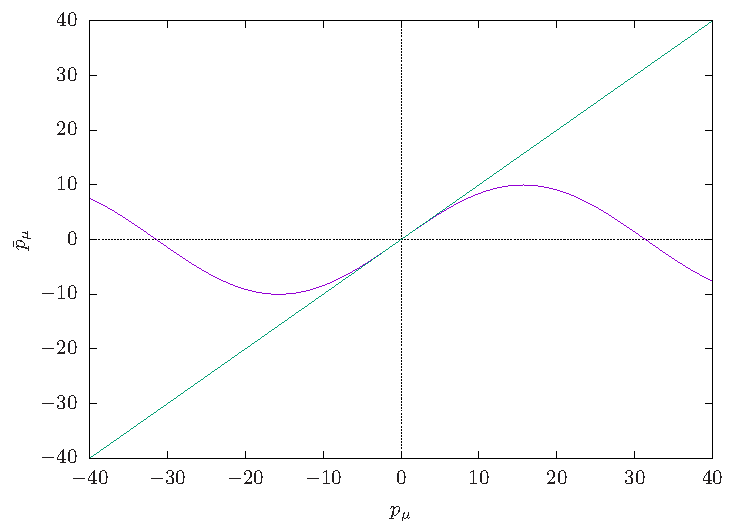
\includegraphics[width = 8 cm]{images/pbar.pdf}
    \caption{Violet curve: $\Bar{p}_\mu = \frac{1}{a} \sin(p_\mu a)$, $a = 0.1$. Green curve: $\Bar{p}_\mu = p_\mu$}
    \label{fig: pbar vs p}
\end{figure} 
Figure (\ref{fig: pbar vs p}) shows how for large momenta, where $p_\mu$ and $\Bar{p}_\mu$ are of the order of $a^{-1}$, the deviation from the $\Bar{p}_\mu = p_\mu$ line is not negligible, and we have high momentum excitations also for $a \to 0$.
The propagator, which in the space regime coincides with the fermionic two-point function, takes contributions from 16 fermion-like particles, which are pure lattice artifacts with no continuum analog.
\\ The origin of doublers has a precise meaning, since it is tangled with the chiral anomaly of our theory.
In the massless fermion limit ($m = 0$), the continuum QED action (\ref{sqed}) is invariant under the global chiral transformation:
\begin{equation}
    \psi \to e^{i\theta \gamma_5} \psi \hspace{15mm} \Bar{\psi} \to \Bar{\psi} e^{i\theta \gamma_5}
\end{equation}
where $\theta$ is a parameter and $\gamma_5 = \gamma_1 \gamma_2 \gamma_3 \gamma_4$ is an hermitian matrix which anticommutes with any $\gamma_\mu$. Since for any global symmetry we expect a conserved current, the global chiral symmetry implies the existence of a conserved axial-vector current, but due to quantum fluctuation it diverges anomalously in the continuum theory. When we regularize the theory on lattice and try to preserve chiral symmetry, we implicitly impose that this current is strictly conserved for any $a$, hence the lattice finds a way to cancel the anomaly of the continuum limit, associated with momentum excitations around $p = 0.$
\\ The appearence of doublers must occur in a lattice regularization which respects $\gamma_5$-hermiticity, locality and translational invariance, as it is formalized in the Nielsen-Ninomiya No Go Theorem \cite{NIELSEN198120}. The theorem states that, given a lattice regularization of the Dirac equation, its kernel $\Tilde{K}(p)$ in momentum space cannot satisfy the following conditions simultaneously:
\begin{enumerate}
    \item $\Tilde{K}(p)$ is a smooth function of momenta $p_\mu$, with period $\frac{2\pi}{a}$.
    \item In the massless fermions limit, $\Tilde{K}(p)$ reduces to the continuum Dirac operator for $a \to 0$.
    \item $\Tilde{K}(p)$ is invertible $\forall p \neq 0.$
    \item In the massless fermions limit, $\Tilde{K}(p)$ satisfies: $\{\Tilde{K}(p), \gamma_5 \} = 0.$
\end{enumerate}
Hence the action (\ref{S naive}) lead to the appearance of doublers because it implicitly required invariance under chiral symmetry! As a consequence, in order to remove these unphysical objects, one needs to sacrifice chiral symmetry. 

\subsection{Wilson fermion}
In this framework, a possible solution was proposed by Wilson. The idea consists in a modification of the Dirac action, such that in the naive continuum limit $a \to 0$ it reduces to the standard formulation and takes care of doublers. As we mentioned before, the price to pay is the breaking of chiral symmetry, which is puzzling but does not spoil the definition of our theory on lattice, as it is a global symmetry of QED rather than a defining one. 
\\ Wilson proposed the following Dirac-operator:
\begin{equation}
    D^{(W)} = \frac{1}{2} \{ \gamma_\mu (D_\mu^* + D_\mu) - r D_\mu^\dagger D_\mu \}
\end{equation}
where $r$ is the so-called Wilson parameter (we will fix $r = 1$ in our case study). This expression differs from the naive discretization of the Dirac operator because of the second term, which is a gauge-invariant discrete version of the euclidean D'Alambertian $\Box$. \\ The Wilson-modified action is then given by:
\begin{equation}
    S_F^{(W)} = a^4 \sum_{n, m \in \Lambda} \Bar{\psi}_\alpha(n) K_{\alpha, \beta}^{(W)}(n, m) \psi_\beta(m)
\end{equation}
with:
\begin{equation}
\begin{split}
        K_{\alpha, \beta}^{(W)}(n, m) & = D^{(W)}_{\alpha, \beta}(n,m) - m \delta_{\alpha, \beta}\delta_{m,n} \\
         & = (m + 2r)\delta_{\alpha, \beta}\delta_{m,n} - \frac{1}{2}\sum_\mu \left[(r - \gamma_\mu)_{\alpha, \beta} \delta_{m, n+\hat{\mu}} + (r + \gamma_\mu)_{\alpha, \beta} \delta_{m, n - \hat{\mu}} \right]
\end{split}
\end{equation}
Notice that for $r \neq 0$, this definition breaks chiral symmetry even for $m \to 0$.
\\ One can prove that the kernel in momentum space $\Tilde{K}^{(W)}(p)$ does not satisfy the anticommuting condition with $\gamma_5$, hence it can obey all the remaining conditions of the Nielsen-Ninomiya theorem. 
In particular, the Dirac-Wilson operator takes care of doublers, because the $\mathcal{O}(a)$ term introduced by Wilson changes the propagator and gives to the unphysical excitations a mass proportional to $a^{-1}$, which diverges for $a \to 0$. 
\\ Indeed, one can show that:
\begin{equation}
    \Tilde{K}_W (p) = i \gamma_\mu \Bar{p}_\mu + m\mathbb{1} + \frac{a}{2} \hat{p}^2 \hspace{4mm} \mbox{with} \hspace{4 mm} \hat{p}_\mu = \frac{2}{a} \sin(\frac{p_\mu a}{2})
\end{equation}
and from an analysis similar to the naive case, the propagator is now given by (in the massless fermions limit $m = 0$):
\begin{equation}
    \frac{-i \gamma_\mu \Bar{p}_\mu + \frac{a}{2} \hat{p}^2}{\sum_\mu \Bar{p}_\mu^2 + (\frac{a}{2} \hat{p}^2)^2}
\end{equation}
In the directions associated with doublers ($p_\mu = \pm \pi/a$), we get $\hat{p}_\mu = \pm 2/a$, hence the mass associated to the unphysical excitation is proportional to $\frac{1}{a} \xrightarrow{a \to 0} \infty$, so that these degrees of freedom decouple from our theory in the continuum limit. The pole in $p = 0$ is the only one with vanishing mass for $a \to 0$, hence Wilson's proposal is a good discretization of the continuum Dirac action.
\\ It is good to remark that there are other working solution in literature, such as \textit{staggered fermions}, but in our work we will deal with Wilson fermions.

\section{Compact QED: Lattice Formulation}
We can finally conclude the construction of the lattice QED action. This process will follow two basic requirements, i.e. the action should be locally invariant under $U(1)$ transformations and should reduce to the classical continuum action in the naive continuum limit.
\\ The QED action should contain a fermion part and a gauge part, just like in the continuum formulation, and we should start with the fermionic term. Recall the lattice action for a free Dirac field:
\begin{equation}
\begin{split}
    & S_F^{(W)} [\psi, \Bar{\psi}] = (m + 2r)\sum_{n \in \Lambda} \Bar{\psi}(n)\psi(n) - \\ & \hspace{20mm} - \frac{1}{2}\sum_{n, \mu} \left[\Bar{\psi}(n)(r - \gamma_\mu)_{\alpha, \beta} \psi(n + \hat{\mu}) + \Bar{\psi}(n + \hat{\mu})(r + \gamma_\mu)_{\alpha, \beta} \psi(n) \right]
\end{split}
\end{equation}
This expression is invariant under the global U(1) transformation:
\begin{equation*}
    \begin{split}
       & \psi(n) \to G\psi(n) \\
       & \Bar{\psi}(n) \to \Bar{\psi}(n) G^{-1}
    \end{split}
\end{equation*}
where $G \in U(1).$ We want to promote this global symmetry to a local one, hence in the previous relations the group element should depend on the lattice site $G(n).$ \\ This could seem to be problematic, as the fermion action includes terms which are non-diagonal in the lattice site, e.g. $\Bar{\psi}(n)\gamma_\mu\psi(n + \hat{\mu})$. Anyway, the puzzle can easily be solved thanks to an idea developed, again, by Wilson: we will introduce new degrees of freedom, which will embed the gauge fields contribution in our theory in a gauge-invariant fashion and will allow us to implement a local $U(1)$ gauge invariance.
\\ Let's see how the problem would be handled in the continuum. Given a bilinear $\Bar{\psi}(x) \psi(y)$, generally it is not invariant under a local gauge transformation:
\begin{equation*}
    \Bar{\psi}(x) \psi(y) \to \Bar{\psi}^G(x) \psi^G(y) = \Bar{\psi}(x) G^{-1}(x) G(y) \psi(y) \Rightarrow G^{-1} (x) G(y) \neq \mathbb{1}
\end{equation*}
In order to make it gauge-invariant, we must compensate the variation $G^\dagger (x) G(y)$ by introducing a factor which depends on the gauge potential, the so called \textit{Schwinger line integral}:
\begin{equation}
    U(x, y) = e^{i\int_x^y dz_\mu A_\mu(z)}
\end{equation}
where $z_\mu$ is a unit vector tangent to the path $C$ connecting $x$ and $y$ (the sum over $\mu$ is understood). One can prove easily that under a gauge transformation $A_\mu \to A_\mu - \frac{1}{e} \partial_\mu A_\mu$, the Schwinger line transforms covariantly:
\begin{equation}\label{bil1}
    U(x, y) \to U^G(x,y) = G(x) U(x, y) G^{-1}(y)
\end{equation}
hence we can build a gauge-invariant object as $\Bar{\psi}(x) U(x, y) \psi(y)$. If we fix $y = x + \varepsilon$ and take $\varepsilon \to 0$, we can expand the previous contraction, and with a little algebra one gets to the result:
\begin{equation}\label{bil2}
    \Bar{\psi}(x) U(x, x + \varepsilon) \psi(x + \varepsilon) = \Bar{\psi}(x) \psi(x) + \varepsilon \Bar{\psi}(x) \left( \partial_\mu + i e A_\mu \right) \psi(x) + \mathcal{O}(\varepsilon^2)
\end{equation}
From this expression, we read that the Schwinger line is essentially a generalization of the covariant derivative when $x$ and $y$ are not at an infinitesimal distance. Since on a lattice our fields are necessarily defined at a finite distance, Wilson conjectured that one could use Schwinger lines as the fundamental degrees of freedom of lattice gauge theories, instead of the gauge fields we used to build the covariant derivative. This will lead to a modification of the gauge action, which is nevertheless legitimate: any regularization on lattice suffers from discretization errors which cancel out in the continuum limit, so one can modify these errors in order to preserve an exact gauge invariance for the action of our theory.
\\ Notice that we are substituting gauge fields, objects which live in the algebra of the gauge group, with Schwinger lines between two adjacent point of the lattice, hence elements of the gauge group. As Schwinger lines connect different points of the lattice, we will also call them \textit{links}. For instance, the discrete form of our gauge field will be given by a $U(1)$ element, which can be written as:
\begin{equation}
    U_\mu (n) = e^{i \phi_\mu (n)}
\end{equation}
where $\phi_\mu$ is a real-valued variable which takes values in $[0, 2\pi]$, and this objects lives on the link connecting the lattice site $n$ to an adjacent one $n + \hat{\mu}$, with $\mu = \{0, 1, 2, 3\}$. One can prove that, in order to have the correct naive continuum limit for the QED action, we can establish a relation between the phase $\phi_\mu(n)$ and the vector potential $A_\mu(n)$, so that we should actually consider the identification\footnote{Note that the identification of $A_\mu(n)$ with the vector potential is strictly true only in the continuum limit.}:
\begin{equation}
    U_\mu (n) = e^{iea A_\mu(n)}
\end{equation}
\begin{center}



\tikzset{every picture/.style={line width=0.75pt}} %set default line width to 0.75pt        

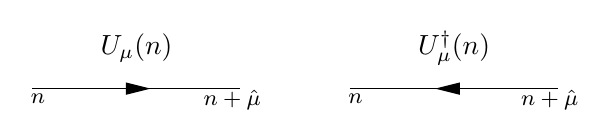
\begin{tikzpicture}[x=0.75pt,y=0.75pt,yscale=-1,xscale=1]
%uncomment if require: \path (0,82); %set diagram left start at 0, and has height of 82

%Straight Lines [id:da540606925296075] 
\draw    (198,40.71) -- (298,40.71) ;
\draw [shift={(255,40.71)}, rotate = 180] [fill={rgb, 255:red, 0; green, 0; blue, 0 }  ][line width=0.08]  [draw opacity=0] (12,-3) -- (0,0) -- (12,3) -- cycle    ;
%Straight Lines [id:da6698465419967881] 
\draw    (351,40.71) -- (451,40.71) ;
\draw [shift={(392,40.71)}, rotate = 0] [fill={rgb, 255:red, 0; green, 0; blue, 0 }  ][line width=0.08]  [draw opacity=0] (12,-3) -- (0,0) -- (12,3) -- cycle    ;


% Text Node
\draw (196,42.11) node [anchor=north west][inner sep=0.75pt]  [font=\footnotesize]  {${\textstyle n}$};
% Text Node
\draw (279.2,40.11) node [anchor=north west][inner sep=0.75pt]  [font=\footnotesize]  {${\textstyle n+\hat{\mu }}$};
% Text Node
\draw (229.6,13.11) node [anchor=north west][inner sep=0.75pt]    {$U_{\mu }( n)$};
% Text Node
\draw (349,42.11) node [anchor=north west][inner sep=0.75pt]  [font=\footnotesize]  {${\textstyle n}$};
% Text Node
\draw (432.2,40.11) node [anchor=north west][inner sep=0.75pt]  [font=\footnotesize]  {${\textstyle n+\hat{\mu }}$};
% Text Node
\draw (382.6,11.61) node [anchor=north west][inner sep=0.75pt]    {$U_{\mu }^{\dagger }( n)$};


\end{tikzpicture}
\end{center}
\\ As we can see in the drawing above, links are directed quantities, so the complex conjugate will be defined as:
\begin{equation}\label{U}
    U_\mu^\dagger(n) = e^{-ieaA_\mu(n)}
\end{equation}
and will connect the lattice site $n + \hat{\mu}$ to $n$. In analogy to what we have described in the continuum formulation in (\ref{bil1})-(\ref{bil2}), the non-diagonal terms of the fermionic action will become:
\begin{equation}
    \begin{split}
        & \Bar{\psi}(n) (r - \gamma_\mu) \psi(n + \hat{\mu}) \to \Bar{\psi}(n) (r - \gamma_\mu) U_\mu(n) \psi(n + \hat{\mu}) \\
        & \Bar{\psi}(n + \hat{\mu}) (r + \gamma_\mu) \psi(n) \to \Bar{\psi}(n + \hat{\mu}) (r + \gamma_\mu) U_\mu^\dagger(n) \psi(n)
    \end{split}
\end{equation}
and these expressions are now invariant under the set of local transformations:
\begin{equation}
    \begin{split}
        & \psi(n) \to G(n) \psi(n) \hspace{33 mm} \Bar{\psi}(n) \to \Bar{\psi}(n) G^{-1} (n) \\
        & U_\mu(n) \to G(n) U_\mu(n) G^{-1}(n + \hat{\mu}) \hspace{10 mm} U_\mu^\dagger(n) \to G(n + \hat{\mu}) U_\mu^\dagger(n) G^{-1}(n)
    \end{split}
\end{equation}
By requiring such transformation laws, we can implement the $U(1)$ gauge invariance naturally. The idea that links should be group elements, rather than elements of the group algebra, comes from the fact that also their gauge transforms must be $U(1)$ elements.
\\ Finally, we can write the gauge invariant action for Wilson fermions on lattice:
\begin{equation}
    \begin{split}
        & S_F^{(W)} [\psi, \Bar{\psi}, U] = (m + 2r) \sum_{n \in \Lambda} \Bar{\psi}(n) \psi(n) - \\
        & \hspace{25 mm} - \frac{1}{2} \sum_{n, \mu} \left[ \Bar{\psi}(n) (r - \gamma_\mu) U_\mu(n) \psi(n + \hat{\mu}) + \Bar{\psi}(n + \hat{\mu}) (r + \gamma_\mu) U_\mu^\dagger(n) \psi(n) \right]
    \end{split}
\end{equation}
and by replacing $U_\mu(n) \simeq 1 + i e a A_\mu(n)$ for small values of $a$, one can show that $S_F^{(W)}$ reduces to the continuum expression in the naive continuum limit.
\\ In order to complete our lattice description of QED, we should now take care of the gauge-invariant discretization of the gauge action, embedding the link variables we just introduced. It turns out that the easiest local object that allows us to build a gauge-invariant realization is the so-called \textit{plaquette}, i.e. the smallest counterclockwise path-ordered product of link variables, as shown below:
\begin{equation}
    U_{\mu\nu}(n) = U_\mu(n) U_\nu(n + \hat{\mu}) U_\mu^\dagger(n + \hat{\nu}) U_\nu^\dagger(n)
\end{equation}
\begin{center}
    
\tikzset{every picture/.style={line width=0.75pt}} %set default line width to 0.75pt        

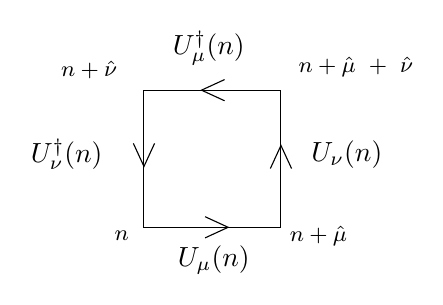
\begin{tikzpicture}[x=0.75pt,y=0.75pt,yscale=-1,xscale=1]
%uncomment if require: \path (0,182); %set diagram left start at 0, and has height of 182

%Shape: Square [id:dp08152467645896022] 
\draw   (297.13,62.23) -- (363.15,62.23) -- (363.15,128.25) -- (297.13,128.25) -- cycle ;
\draw   (326.6,123.23) -- (337.72,128.34) -- (326.6,133.45) ;
\draw   (336,57.17) -- (324.88,62.27) -- (336,67.38) ;
\draw   (302.27,87.92) -- (297.16,99.03) -- (292.05,87.92) ;
\draw   (358.05,100.03) -- (363.16,88.92) -- (368.27,100.03) ;


% Text Node
\draw (281.8,128.91) node [anchor=north west][inner sep=0.75pt]  [font=\footnotesize]  {${\textstyle n}$};
% Text Node
\draw (366.2,126.31) node [anchor=north west][inner sep=0.75pt]  [font=\footnotesize]  {${\textstyle n+\hat{\mu }}$};
% Text Node
\draw (312.2,136.11) node [anchor=north west][inner sep=0.75pt]    {$U_{\mu }( n)$};
% Text Node
\draw (370.4,45.23) node [anchor=north west][inner sep=0.75pt]  [font=\footnotesize]  {${\textstyle n+\hat{\mu } \ +\ \hat{\nu }}$};
% Text Node
\draw (256,47.23) node [anchor=north west][inner sep=0.75pt]  [font=\footnotesize]  {${\textstyle n+\hat{\nu }}$};
% Text Node
\draw (376.6,85.23) node [anchor=north west][inner sep=0.75pt]    {$U_{\nu }( n)$};
% Text Node
\draw (309.8,32.43) node [anchor=north west][inner sep=0.75pt]    {$U_{\mu }^{\dagger }( n)$};
% Text Node
\draw (241.4,84.43) node [anchor=north west][inner sep=0.75pt]    {$U_{\nu }^{\dagger }( n)$};

\end{tikzpicture}
\end{center}
Using the expression for $U_\mu(n)$ (\ref{U}), one can show that the plaquette reduces to:
\begin{equation}
    U_{\mu\nu}(n) = e^{iea^2F_{\mu\nu}(n)}
\end{equation}
where $F_{\mu\nu}$ is a discretization of the continuum electromagnetic field strength tensor:
\begin{equation}
    F_{\mu\nu}(n) = \frac{1}{a}\left[(A_\nu(n + \hat{\mu}) - A_\nu(n)) - (A_\mu(n + \hat{\nu}) - A_\mu(n)) \right]
\end{equation}
In order to reproduce the continuum action (\ref{S_G}), we need to take a particular combination:
\begin{equation}
    \frac{1}{e^2} \sum_n \sum_{\substack{\mu, \nu \\ \mu < \nu}} \left[1 - \frac{1}{2} \left(U_{\mu\nu}(n) + U_{\mu\nu}^\dagger(n)\right) \right] \approx \frac{1}{4} \sum_{\substack{n \\ \mu, \nu}} a^4 F_{\mu\nu}(n) F_{\mu\nu}(n)
\end{equation}
which can be recast more compactly as:
\begin{equation}
    S_G [U] = \frac{\beta}{2} \sum_P \left[1 - \Re{U_P} \right]
\end{equation}
with $\beta = 2/e^2$, and the sum over $P$ labels a summation over all the plaquettes of the lattice. Comparing this expression with the continuum formulation of QED, one can notice that the coupling constant now appears as $1/e$ in the gauge action, rather than with a linear dependence in the fermionic part. This suggests that the strong coupling expansion is the most natural one in the lattice formulation of the theory.
\\ Now we can write the lattice action for QED with Wilson fermions, which will be at the base of our path-integral formalism:
\begin{equation}\label{S qed lattice}
    \begin{split}
       & S_{QED} [\psi, \Bar{\psi}, U] = S_G[U] + S_F^{(W)} [\psi, \Bar{\psi}] = \\
       & \hspace{23 mm} = \frac{\beta}{2} \sum_P \left[1 - \Re{U_P} \right] + (m + 2r) \sum_{n \in \Lambda} \Bar{\psi}(n) \psi(n) - \\
       & \hspace{36 mm} - \frac{1}{2} \sum_{n, \mu} \left[ \Bar{\psi}(n) (r - \gamma_\mu) U_\mu(n) \psi(n + \hat{\mu}) + \Bar{\psi}(n + \hat{\mu}) (r + \gamma_\mu) U_\mu^\dagger(n) \psi(n) \right] \\
    \end{split}
\end{equation}
The QED partition function will involve an integration over all possible fermionic and gauge fields configurations. The fermionic measure is given by the integration over two sets of Grassmann variables $[\psi, \Bar{\psi}]$, while the link variables $U_\mu(n)$ are elements of the unitary group $U(1)$, so we are integrating over a compact group manifold, which in this case is parameterised by a single real-valued variable $\phi_\mu(n)$ restricted to the range $[0, 2\pi]$. \\ Then we can build the gauge-invariant measure:
\begin{equation}
    \mathcal{D}U \equiv \prod_{n, \mu} d\phi_\mu(n)
\end{equation}
and the QED partition function is given by:
\begin{equation}
    Z_{QED} = \int \mathcal{D}U \mathcal{D}\psi \mathcal{D}\Bar{\psi} \, e^{-S_{QED}[\psi, \Bar{\psi}, U]}
\end{equation}
As a final remark, when we build an interacting theory from this partition function, we shall remember that the parameters $m$ and $e$ that appear in (\ref{S qed lattice}) cannot be interpreted as the physical fermion mass and electric charge, but should rather be regarded as bare parameters with no direct physical meaning.
\\ This completes the review of the theoretical framework of this thesis, so now we can focus more in detail on the case study of our work, the Schwinger Model.
\chapter{HMC Algorithm for the Schwinger Model}
\label{chap: HMC}

In this chapter we will introduce the case study of this thesis, the Schwinger Model. We previously stated the similarities between this two-dimensional realization of QED and the QCD, hence it will be an efficient toy model for the study of the factorization of the fermionic determinant we want to investigate. Nevertheless, in this first part we should focus on a standard realization of the Schwinger Model on lattice.
\\ Once that we have defined the system we want to simulate, we will give a brief overview of the main properties of the Hybrid Monte Carlo Algorithm, i.e. the algorithm we embed to implement the time evolution of our system. 
\\ Consequently, we will adapt the aforementioned algorithm to our case study, giving all the computational details.
\\ Finally, we will report the results of the tests embedded for the standard Schwinger Model (i.e. with no pre-conditioning), in particular how we gauged the acceptance rate of the HMC algorithm, which must be sufficiently high in the following simulations, where we will actually compute some fermionic observables. 

\section{Schwinger Model}
The Schwinger Model is a two-dimensional realization of QED (QED$_2$), hence a system with $U$(1) gauge symmetry and two mass-degenerate dynamical quarks.
\\ Consider a lattice with $L_0$ thick time slices and spatial extension $L_1$. The space-time points of our lattice $\Lambda$ are labelled by two-integers vectors $n$:
\begin{equation}\label{lattice 2d}
\begin{split}
        \Lambda = \{ n = (n_1, n_2)  | 
        \,\, 0 \leq n_1 \leq L_0 - 1, \,\,\,
        0 \leq n_2 \leq L_1 - 1 \}
\end{split}
\end{equation}
\\ Periodic boundaries conditions (PBC) will be employed in both directions for bosonic degrees of freedom, while fermions will endow PBC along the spatial coordinate and anti-periodic boundary conditions (APBC) in the time direction.
\\ In our lattice formulation we will embed the previously described Wilson-fermions, hence the fermionic part of the action is given by:
\begin{equation}
\begin{split}
    S_F [\psi, \Bar{\psi}, U] &= (m_0 + 2r) \sum_{n, \alpha} \Bar{\psi}_\alpha(n)\psi_\alpha(n) -  \\  
        & - \frac{1}{2}\sum_{\substack{n, \mu \\ \alpha, \beta}}\left[ \Bar{\psi}_\beta(n)(r - \gamma_\mu)_{\beta, \alpha} U_\mu(n) \psi_\alpha(n + \hat{\mu}) + \Bar{\psi}_\beta (n+\hat{\mu}) (r + \gamma_\mu)_{\beta, \alpha} U^\dagger_\mu(n) \psi_\alpha(n) \right] \\
\end{split}
\end{equation}
where $\alpha$ and $\beta$ label the components of the fermionic fields, $m_0$ is the bare mass parameter, we set the Wilson parameter $r = 1$, and $\gamma_\mu$ are the two-dimensional realization of gamma matrices ($\mu = 0, 1$).
In the Dirac basis, $\gamma$-matrices can be written as:
\begin{equation}\label{gammas}
    \gamma_0 = - \sigma_3 = \begin{pmatrix}
 -1 & 0  \\
   0 & 1 \\
\end{pmatrix}
   \,\,\,\,\,\, \gamma_1 = \sigma_1 = \begin{pmatrix}
 0 & 1  \\
   1 & 0 \\
\end{pmatrix}
   \,\,\,\,\,\, \gamma_2 = i\gamma_0 \gamma_1 = \sigma_2 = \begin{pmatrix}
 0 & -i  \\
   i & 0 \\
\end{pmatrix}
\end{equation}
where $\sigma_i$ ($i = 1, 2, 3$) are the Pauli matrices. Analogously to what we have seen before, we can define the Dirac-Wilson operator acting on two quarks defined in $m$ and $n$ as:
\begin{equation}\label{D}
\begin{split}
        D_{\beta, \alpha} (m, n) = &(m_0 + 2) \delta_{\beta, \alpha} \delta_{m,n} - \\ &- \frac{1}{2}\sum_{\mu} \left[ (1 - \gamma_\mu)_{\beta, \alpha} U_\mu(m) \delta_{n, m+\hat{\mu}} + (1 + \gamma_\mu) U_\mu^\dagger (m - \mu)_{\beta, \alpha} \delta_{n, m - \hat{\mu}} \right]
\end{split}
\end{equation}
This operator satisfies the so called $\gamma_2$-hermiticity, hence:
\begin{equation}
    D^\dagger = \gamma_2 D \gamma_2
\end{equation}
and the Hermite-conjugate of the Dirac operator can be written as:
\begin{equation}\label{D daga}
\begin{split}
         D^\dagger_{\beta, \alpha} (m, n) & = (m_0 + 2) \delta_{\beta, \alpha} \delta_{m,n} - \\ 
         & - \frac{1}{2}\sum_{\mu} \left[ (1 - \gamma_\mu)_{\beta, \alpha} U_\mu^\dagger(m - \mu) \delta_{n, m - \hat{\mu}} + (1 + \gamma_\mu)_{\beta, \alpha} U_\mu (m) \delta_{n, m + \hat{\mu}} \right]
\end{split}
\end{equation}
Finally, the fermionic action can be rewritten as:
\begin{equation}
\begin{split}
    S_F[\psi, \Bar{\psi}, U] & = \sum_{\substack{n, m \\ \alpha, \beta}} \Bar{\psi}_\beta(m) D_{\beta, \alpha}(m, n) \psi_\alpha(n) = \\
    & = \sum_{n, \alpha} \Bar{\psi}_\alpha(n) \psi_\alpha(n) - \kappa \sum_{n, \mu} \left[ \Bar{\psi}(n)(1 - \gamma_\mu) U_\mu(n) \psi(n+\hat{\mu}) + \right. \\ & \hspace{40mm} \left. + \Bar{\psi}(n)(1 + \gamma_\mu) U_\mu^\dagger (n - \mu) \psi(m - \hat{\mu}) \right]
\end{split}
\end{equation}
where $\kappa = \frac{1}{2(m_0 + 2)}$.
For what concerns the gauge part, the action is given by:
\begin{equation}\label{Sg}
        S_G[U] = -\beta \sum_{P} \Re{U_P}
\end{equation}
where
\begin{equation*}
    U_P(n) = U_\mu(n) U_\nu (n + \hat{\mu}) U^\dagger_\mu(n+\hat{\nu}) U^\dagger_\nu(n) = U_0(n) U_1 (n + \hat{0}) U^\dagger_0(n+\hat{1}) U^\dagger_1(n)
\end{equation*}
is the standard plaquette in (1+1) dimensions. Recall that $U_\mu(n) \in U(1)$ is a link-variable connecting points $n$ and $n + \hat{\mu}$ of the lattice, with $\mu = 0, 1$.
Accordingly to the current state of art of computatational techniques for lattice gauge theories, in order to simulate our system we first require to integrate out analytically the fermionic degrees of freedom. Since we are working with two mass-degenerate quark flavors, the partition function is given by:
\begin{equation*}
    Z = \int \mathcal{D}[U]\, e^{-S_G[U]} \det[D] \det[D]
\end{equation*}
We can recast this expression in order to obtain an effective gauge theory which can be simulated through Monte Carlo algorithms, where we exploit gauge configuration properly distributed according to the gauge action. Nevertheless, this process comes with downsides, as the locality of the original action is not manifest anymore, as the fermion determinant is a non-local functional of the links $U$. 
\\ In our simulations, accordingly to the previous expression, we can interpret the fermion determinant as a probability weight factor when generating gauge configurations, since it is real (thanks to $\gamma_2$-hermiticity) and non-negative. Hence we will define a Monte Carlo algorithm which draws gauge configurations with the following probability distribution:
\begin{equation*}
    \frac{1}{Z}\,e^{-S_G[U]} \det[D] \det[D] =  \frac{1}{Z}\,e^{-S_G[U]} \det[D D^\dagger]
\end{equation*}
To introduce a bosonic effective action, we can express $\det[DD^\dagger]$ as the result of a bosonic Gaussian integral over $N$ complex variables $\phi$:
\begin{equation}
    \det[DD^\dagger] =  \pi^{-N} \int \mathcal{D}[\phi_R] \mathcal{D}[\phi_I] \, e^{-\phi^\dagger (DD^\dagger)^{-1} \phi}
\end{equation}
and we refer to $\phi$ as pseudofermion fields, i.e. bosons with the same number of degrees of freedom as fermions. If the number of mass-degenerate fermions is even, we can guarantee positivity, hence the convergence of the Gaussian integral.
\\ Then we can define the \textit{effective fermion action}:
\begin{equation}
    S_F^{\textrm{eff}} [U] = \phi^\dagger (DD^\dagger)^{-1} \phi
\end{equation}
which is highly non-local, as it basically connects all the link variables of the lattice with each other.
In conclusion, a possible way to include dynamical fermions in our simulations consists in generating gauge configurations in our Markov Chain accordingly to the Boltzmann weight factor:
\begin{equation}
    \exp(-S[U]) \hspace{10mm} \mbox{with:} \hspace{2mm} S[U] = S_G[U] + S_F^{\textrm{eff}} [U]
\end{equation}
In the next chapter we introduce the algorithm typically used (within its variants) for the simulation of lattice gauge theories, the Hybrid Monte Carlo (HMC) algorithm \cite{DUANE1987216}.  

\section{Hybrid Monte Carlo}
This algorithm is based on the concept of Markov Chains, hence a sequence of configurations-drawings which represent the dynamical evolution of our system in the computer time (or \textit{Markov time}, $\tau$), accordingly to the desired probability distribution $\exp(-S[U])$.
\\ The name \textit{hybrid} comes from the fact that the candidates for the new gauge-configurations come from the evolution of classical Molecular Dynamics (MD) equations of motion, and the algorithm is completed by a following step where the proposal gets accepted or rejected as in the Metropolis-Hastings algorithm. Let us see these two steps more in detail.
\\ The overall transition probability from one configuration to the following one is given by two terms. Starting from a gauge configuration $U$, through the MD leapfrog evolution scheme we will propose a new candidate $U'$, introducing an a priori selection probability factor $T_0(U' | U)$. Nextly, we decide whether to accept the proposal accordingly to the acceptance probability:
\begin{equation}
    T_A (U'|U) = \min \left(1, \frac{T_0(U|U') e^{-S[U']}}{T_0(U'|U) e^{-S[U]}}\right)
\end{equation} 
Putting all together, the overall transition probability is:
\begin{equation*}
    T(U'|U) = T_A(U'|U)T_0(U'|U)
\end{equation*}
Since we are interested in ergodic Markov Chains, we require this probability to obey the detailed balance condition:
\begin{equation}
    T(U'|U) P(U) = T(U|U')P(U')
\end{equation}
hence the probability of drawing the configuration $U$ and transitioning from $U \to U'$ must be equal to the probability of drawing $U'$ and then evolve $U' \to U.$ An explicit proof of the fact that the HMC algorithm satisfies the detailed balance condition can be found in Appendix \ref{app:a}.
\subsection{HMC Algorithm for the Schwinger Model}
Here we will show more in-depth the steps of the algorithm for our case study.
\\ Consider the system described previously, with the introduction of pseudofermion fields $\phi$. We want to draw configurations distributed accordingly to the Boltzmann weight factor:
\begin{equation}
    \exp(-S[U]) = \exp(\beta \sum_P \Re{U_P} - \phi^\dagger (DD^\dagger)^{-1}\phi )
\end{equation}
and in our evolution scheme, pseudofermion fields and gauge fields will be updated alternatively. The dynamical evolution of this system is given by the following steps.
\begin{itemize}
    \item \textbf{Step 1 (Pseudofermions):} We want to generate pseudofermion fields according to the Gaussian distribution $e^{- \phi^\dagger (D D^\dagger )^{-1} \phi}$. To achieve this, we can generate a complex vector $\chi$ according to a Gaussian distribution $e^{-\chi^\dagger\chi}$, and then compute $\phi = D\chi$.
    \\ Pseudofermion fields will be kept fixed during the time evolution of the gauge fields.
    \item \textbf{Step 2 (Conjugate variables)}: We will consider as conjugate variables the gauge fields $U_\mu(n)$ and a set of momenta $\pi_{\mu}(n)$ distributed according to a Gaussian $e^{-\Pi^2/2}$. Notice that $U_\mu(n)$ is a $U(1)$ group element, i.e. a phase factor, and it can be written as: 
    \begin{equation*}
        U_\mu(n) = \exp(iQ_\mu(n)) \,\,\,\,\mbox{with }\,\, n \in \Lambda, \, \mu = 0,1  \,\,\mbox{and}\,\,\,Q_\mu \,\,\mbox{real}
    \end{equation*}
    \item \textbf{Step 3 (Leapfrog equations):} The classical set of equations of motions for conjugate variables $Q$ and $\pi$ such that $H[Q, \pi] = \frac{1}{2} \pi^2 + S[Q]$ is:
    \begin{equation}\label{EOM}
    \begin{split}
        \dot{Q} &= \pdv{H}{\pi} = \pi \\
        \dot{\pi} &= -\pdv{H}{Q} = - \pdv{S}{Q}
    \end{split}
    \end{equation}
    where the derivatives understand a derivation with respect to a field value at a single lattice site.
    \\ These equations of motion are derived by asking $\Dot{H} = 0$, hence that the Hamiltonian is a constant of motion. If we could implement the dynamical evolution exactly, the proposals for the gauge configurations would always be accepted, but this is not the case, since the evolution scheme will be integrated numerically. 
   \\ Nevertheless, by following the so-called leapfrog integration scheme, we can derive a dynamical evolution which satisfies the detailed balanced condition, since the MD trajectory is reversible.\footnote{Reversibility is given by the condition: $T(Q', \pi'|Q, P) = T (Q, -\pi|Q', -\pi')$. In order to satisfy the detailed balance condition, the MD trajectory must also guarantee the area preservation of the integration measure $\mathcal{D}[\pi]\mathcal{D}[Q]$.}.
    \\ To integrate the classical equations of motion, we will implement a numerical integral with a discrete step size $\varepsilon = \Delta \tau$. 
    \\ The real phases $Q$ are evolved in $n$ steps of length $\varepsilon$, while the conjugate momenta $\pi$ start with a half-step $\varepsilon/2$, then they undergo $(n-1)$ full steps and finally again a half-step. Iterating this steps we build a molecular dynamics trajectory: we can combine $n$ leapfrog steps to build a trajectory of length $n \varepsilon \simeq 1$. 
    \\ Since we are integrating these equations numerically, the evolution scheme is only approximately correct, as numerical errors must be taken into account: the discretization error for half-steps is $\mathcal{O}(\varepsilon^2)$, for full steps it is $\mathcal{O}(\varepsilon^3)$. 
    \\ In the next subsection we will compute the integration scheme explicitly.
    \item \textbf{Step 4 (Accept/Reject)}: Once that the final step of the trajectory is reached, we accept the proposal $(Q(\tau), \pi(\tau)) \to (Q(\tau + n\varepsilon), \pi(\tau + n \varepsilon)) \equiv (Q', \pi')$ if:
    \begin{equation*}
        r < \frac{\exp{-H[Q(\tau + n\varepsilon), \pi(\tau + n\varepsilon)]}}{\exp{-H[Q(\tau), \pi(\tau)]}}
    \end{equation*}
    where $r$ is a random number in $[0,1).$
\end{itemize}
\subsection{Leapfrog evolution scheme}
In the previous section we have seen the molecular dynamics equations (\ref{EOM}), now we want to solve them explicitly for our system. To keep track of the evolution in the computer time $\tau$, we add an extra label $k = 0, \dots, n$ that denotes the particular evolution step at which we evaluate the variables. For the sake of clarity, $x \in \Lambda$ will now refer to space-time points of the lattice.
\\ \textbf{First step:} We start with a half-step for the evolution of the conjugate momenta $\pi$, and from (\ref{EOM}):
\begin{equation}\label{first step pi}
    \pi_{\mu,0}(x) \to \pi_{\mu, \frac{1}{2}}(x) =  \pi_{\mu,0}(x) - \left. \pdv{S}{Q_\mu(x)} \right\rvert_{Q_{\mu, 0}} \frac{\varepsilon}{2}
\end{equation}
We need to evaluate the derivative of the action $S[U] = S_G[U] + \phi^\dagger (D D^\dagger )^{-1} \phi$ with respect to $Q_\mu$. For what concerns the gauge action, recall that:
\begin{equation*}
\begin{split}
    \Re{U_P} & = \frac{1}{2}(U_P + U_P^\dagger) = \\
             & = \frac{1}{2} \left[  U_\mu(n) U_\nu (n + \hat{\mu}) U^\dagger_\mu(n+\hat{\nu}) U^\dagger_\nu(n) + U_\nu(n) U_\mu (n + \hat{\nu}) U^\dagger_\nu(n+\hat{\mu}) U^\dagger_\mu(n) \right] \\
\end{split}
\end{equation*}
and:
\begin{equation*}
    \begin{split}
        & U_\mu(n) = \exp(iQ_\mu(n)) \\
        & U_\mu^\dagger(n) = \exp(-iQ_\mu(n)) \\
    \end{split}
\end{equation*}
so that the derivative of the gauge action (\ref{Sg}) is given by:
\begin{equation}
\begin{split}
    \pdv{S_G[U]}{Q_0(x)} &= - i \, \frac{\beta}{2} \left[ U_P(x) - U_P^\dagger(x) - U_P(x - \hat{1}) + U_P^\dagger(x - \hat{1}) \right]   \\
                         &= \beta \Im{U_P(x) - U_P(x - \hat{1})} \\
    \pdv{S_G[U]}{Q_1(x)} &= - i \, \frac{\beta}{2} \left[ - U_P(x) + U_P^\dagger(x) + U_P(x - \hat{0}) - U_P^\dagger(x - \hat{0}) \right]   \\
                         &= \beta \Im{- U_P(x) + U_P(x - \hat{0})}                         
\end{split}
\end{equation}
and the plaquettes will be computed with the gauge configuration specified by the evolution step (i.e. for the first step, $Q_{\mu,0}(x)$).
\\ For the fermionic part, since the pseudofermions $\phi$ are kept fixed during the leapfrog evolution:
\begin{equation*}
    \pdv{S_{pf}}{Q_\mu(x)} = \phi^\dagger \, \pdv{(D D^\dagger)^{-1}}{Q_\mu(x)} \, \phi
\end{equation*}
To derive an inverse matrix, we can make use of the relation:
\begin{equation*}
    \pdv{M^{-1}}{\omega} = - M^{-1}\, \left(\pdv{M}{\omega} \right) \, M^{-1}
\end{equation*}
so that we can write:
\begin{equation*}
\begin{split}
       \phi^\dagger \, \pdv{(D D^\dagger)^{-1}}{Q_\mu(x)} \, \phi & = - \phi^\dagger \, (D D^\dagger)^{-1} \pdv{(D D^\dagger)}{Q_\mu(x)} \, (DD^\dagger)^{-1} \phi \\
        & = - \left[(DD^\dagger)^{-1} \phi \right]^\dagger \,  \left[ \pdv{(D)}{Q_\mu(x)}D^\dagger + D \pdv{(D^\dagger)}{Q_\mu(x)} \right]  \, \left[(DD^\dagger)^{-1} \phi \right]
\end{split}
\end{equation*}
If we call:
\begin{equation*}
    \eta(x) = (DD^\dagger)^{-1} \phi(x)
\end{equation*}
and notice that:
\begin{equation*}
    \pdv{D}{Q_\mu(x)}D^\dagger = \left(D \pdv{D^\dagger}{Q_\mu(x)} \right)^\dagger
\end{equation*}
we can rewrite the derivative of the pseudofermion action as:
\begin{equation}
    \pdv{S_{pf}[U]}{Q_\mu(x)} = - 2 \Re{\eta^\dagger(y) \left(\pdv{D}{Q_\mu(x)}D^\dagger\right) (y,z)\, \eta(z)  }
\end{equation}
The drift force of the time evolution is then given by:
\begin{equation}
\begin{split}
    \pdv{S[U]}{Q_0(x)} &= \beta \Im{U_P(x) - U_P(x - \hat{1})} - 2 \Re{\eta^\dagger(y) \left(\pdv{D}{Q_0(x)}D^\dagger\right) (y,z)\, \eta(z)}   \\
    \pdv{S[U]}{Q_1(x)} &= \beta \Im{- U_P(x) + U_P(x - \hat{0})} - 2 \Re{\eta^\dagger(y) \left(\pdv{D}{Q_1(x)}D^\dagger\right) (y,z)\, \eta(z)} 
\end{split}
\end{equation}
and the computation of the explicit form is reported in Appendix \ref{app:b}.
\\ \textbf{Intermediate steps:} Now we perform $n-1$ full steps for the evolution of $U$ and $\pi$. To see how the link variables evolve, notice that, from the first equation of motion in (\ref{EOM}):
\begin{equation}\label{first step Q}
    Q_{\mu,1}(x) = Q_{\mu, 0}(x) + \varepsilon \pi_{\mu,\frac{1}{2}}(x)
\end{equation}
and since 
\begin{equation*}
    U_{\mu,0}(x) = \exp(iQ_{\mu,0}(x)) \to Q_{\mu, 0}(x) = -i \ln(U_{\mu, 0})(x)
\end{equation*}
one easily finds that:
\begin{equation*}
    U_{\mu, 1}(x) = \exp(i\varepsilon \pi_{\mu, \frac{1}{2}} (x))\, U_{\mu, 0}(x)
\end{equation*}
Generalizing for the intermediate full-steps, we find:
\begin{equation}
    \begin{split}
        U_{\mu, k}(x) = \exp(i\varepsilon \pi_{\mu, k - \frac{1}{2}} (x))\, U_{\mu, k-1}(x) \\
        \pi_{\mu, k + \frac{1}{2}}(x) = \pi_{\mu, k - \frac{1}{2}}(x) - \varepsilon \left. \pdv{S}{Q_\mu(x)} \right\rvert_{Q_{\mu, k}} \\
    \end{split}
\end{equation}
with $k = 1, \dots, n-1$.
\medskip
\\ \textbf{Final step:} We conclude the MD trajectory with a full step for the gauge fields and an half-step for the momenta, hence:
\begin{equation}
    \begin{split}
        U_{\mu, n}(x) = \exp(i\varepsilon \pi_{\mu, n - \frac{1}{2}} (x))\, U_{\mu, n-1}(x) \\
        \pi_{\mu, n}(x) = \pi_{\mu, n - \frac{1}{2}}(x) - \frac{\varepsilon}{2} \left. \pdv{S}{Q_\mu(x)} \right\rvert_{Q_{\mu, n}} \\
    \end{split}
\end{equation}
\subsection{Accept/Reject}
The numerical integration of the equations of motion introduces $\mathcal{O}(\varepsilon^2)$ discretization errors, resulting in an approximately correct evolution. In order to obtain a deterministic process for the dynamical realization of our system we then need a corrective step.
\\ If we denote the initial phase-space point of the MD trajectory as $(P,Q)$, and the final one as $(P', Q')$, then the new configuration must be accepted with probability:
\begin{equation*}
    T_A(P',Q' | P, Q) = \min \left(1, e^{-\Delta H} \right) \hspace{8mm} \mbox{with:} \hspace{2mm} \Delta H = H[P', Q'] - H[P, Q]
\end{equation*}
Operatively, one can prove that the gauge configurations are drawn with the desired probability distribution if the proposal gets accepted if and only if a number drawn from the uniform distribution in the unit interval $r \in [0, 1)$ is such that:
\begin{equation}
\begin{split}
        r < \exp \left(-\pi_n^2 + \pi_0^2 \right. & - S_G[U_n] + S_G[U_0] - \\ 
       & \left. -\phi^\dagger(D[U_n]D^\dagger[U_n])^{-1} \phi + \phi^\dagger(D[U_0]D^\dagger[U_0])^{-1} \phi \right) \\
\end{split}
\end{equation}
For the pseudofermion contribution in the accept-reject step, we can exploit the computation of $(DD^\dagger)^{-1}\phi$ done while computing the drift force in the last evolution step of the leapfrog scheme.

\section{Preliminary Studies}
In this section we will review some of the tests we implemented for our algorithm before we moved on to the actual computation of observables.
\\ As a first step, we investigated the dependence of the acceptance rate of the HMC algorithm on some parameters, namely the discrete MD step $\varepsilon$ and the volume $V = L_0 L_1$.
\begin{figure}
    \centering
    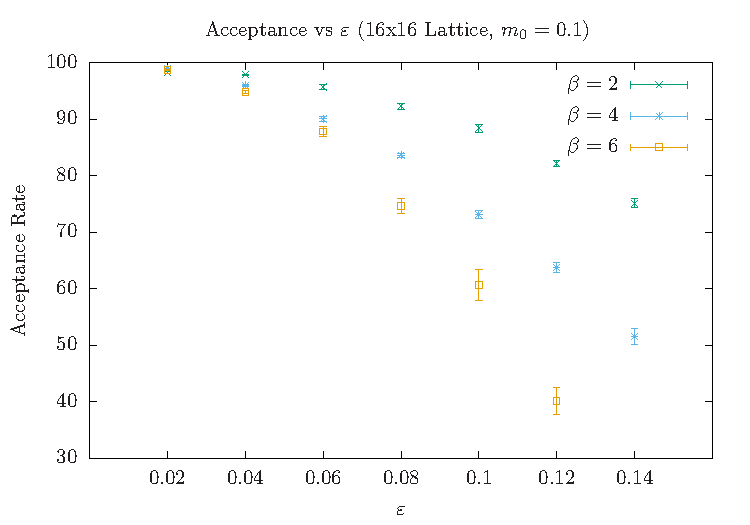
\includegraphics{images/acceps.pdf}
    \caption{Acceptance rate vs $\varepsilon$}
    \label{fig:acc_eps}
\end{figure}
\begin{figure}
    \centering
    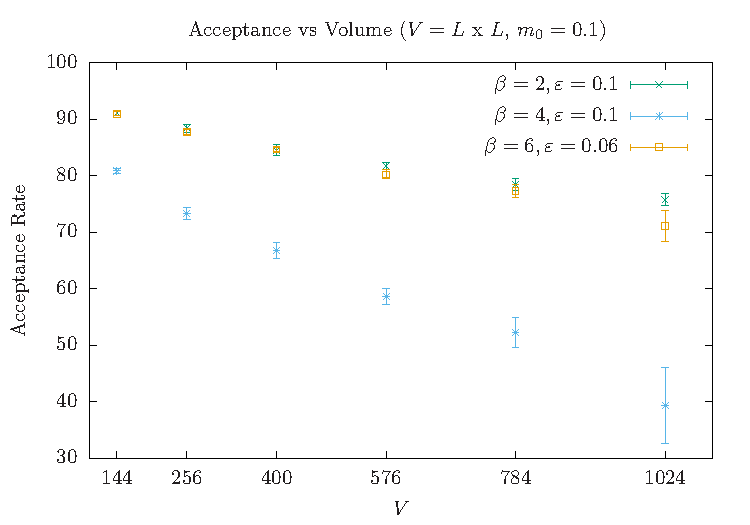
\includegraphics{images/accvol.pdf}
    \caption{Acceptance rate vs $V$}
    \label{fig:acc_vol}
\end{figure}
\\ It is important to work with a sufficiently high acceptance rate, so that one does not waste too much computational resources when taking measurements, hence we need to understand which parameters best fit our requests.
In Figure \ref{fig:acc_eps} we show the dependence of the acceptance rate on the molecular dynamics parameter $\varepsilon$ for a $16 \times 16$ lattice with $m_0 = 0.1$, simulated for different values of the gauge coupling $\beta = 1/g^2$. For small values of $\varepsilon$, the configuration proposed at the end of the trajectory is not that far from the previous one, so it is more likely to be accepted and indeed the acceptance rate is high, independently from the value of $\beta$. As soon as we start to increase the value of $\varepsilon$, the acceptance rate starts decaying quite rapidly: one can clearly see that the acceptance rate falls at a higher pace for smaller values of $\beta.$ 
\\ In Figure \ref{fig:acc_vol} we show the dependence of the acceptance rate on the volume: we simulated square lattices ($L \times L$) with $m_0 = 0.1$ and for different values of the gauge coupling. Notice that for $\beta = 2$ and $4$ we fixed $\varepsilon = 0.1$, while for $\beta = 6$ we embedded a lower value for $\varepsilon$, since simulations with $\varepsilon = 0.1$ produced very low acceptance rates. Coincidentally, in this way we tuned the acceptance rates of the lattices with $\beta = 2$ and $\beta = 6$, and it shows how their dependence on the volume is pretty similar.
\\ Generally, one can conclude that the acceptance rate has a softer dependence on the volume, as it does not decay that rapidly.
Given the above results, we tried to adapt our model parameters in order to always have an acceptance rate of at least $\sim 70\%.$

\chapter{Numerical study}
\label{chap: Std Schwinger Model}

As we mentioned earlier in this paper, the Schwinger model (QED$_2$) is a subject of interest in computational physics since it can lead to a broader understanding of some aspects of QCD$_4$, in particular for what concerns the study of the chiral limit of the theories. 
\\ In our case study we implemented dynamical fermions thanks to the introduction of Wilson fermions, which suffer from an explicit breaking of the chiral $SU(2)_A \times U(1)_A$ symmetries, but we expect the chiral symmetry to be restored at a critical fermion coupling $\kappa_c(\beta).$
\\ In this Chapter, after a brief overview about stochastic estimators typically used in LQCD simulations, the so-called \textit{noise vectors}, we will present some tests conducted on our system in order to investigate more deeply the chiral limit of the Schwinger model.
\\ For instance, the low lying spectrum of the Schwinger model with two mass-degenerate fermions contains an iso-triplet of light particles (which we denote as "pions" $\pi$ by analogy to QCD), which become massless in the chiral limit, and a massive iso-singlet state (the "$\eta$" meson), which leads to a $U(1)$ problem analogous to the one we study in QCD$_4$.\footnote{For $N_f$ massless quarks, QED$_2$ would show one massive and $N_f - 1$ independent massless bosons.}
\\ The first step of our investigation consists in understanding how to reach the chiral limit, i.e. how to fine-tune the bare parameters of our system in order to drive the quark mass (and the pions' mass) to zero. The quark mass $m$ is defined through the implementation of a PCAC relation \cite{Hip_1998}, so that we can study the critical fermion coupling $\kappa_c(\beta)$ at which chiral symmetry is restored, since there is not a simple order parameter which allows us to identify that point in coupling phase space.
\\ Consequently, we focus on the aforementioned low-lying spectrum, retrieving the $\pi$'s and $\eta$ masses from the study of \textit{two point correlation functions}. We compare the results with some simulations in literature \cite{Hip_1998, Gattringer_1999, Christian_2006, https://doi.org/10.48550/arxiv.2201.08008}, as well as for analytical predictions \cite{BELVEDERE1979112, https://doi.org/10.48550/arxiv.hep-th/9505168, Hosotani_1998}.
\\ This tests are useful to pave the way for a future comparison between the standard Schwinger Model simulations and simulations where we embed the fermion determinant factorization we will discuss in the following chapters.


\section{Chiral Condensate and Noise Vectors}
As we stated before, the massive Schwinger Model is an instructive framework, as it shares various non-perturbative features with QCD. For instance, it is embedded with a non-vanishing \textit{chiral condensate}, which for a $L_0 \times L_1 = V$ lattice with $N_f$ quark flavors it is defined as:
\begin{equation}\label{cc}
    \Sigma = - \langle \Bar{\psi} \psi \rangle = - \frac{1}{V} \frac{1}{N_f} \sum_x \sum_{i = 1}^{N_F} \langle \Bar{\psi}_i (x) \psi_i(x) \rangle 
\end{equation}
where $\langle \dots \rangle$ here denotes an expectation value taken over fermionic degrees of freedom and over different gauge configurations. For what concerns the fermionic expectation value, we can use Wick's theorem:
\begin{equation}
    \langle \Bar{\psi}_i(x) \psi_i (x) \rangle_F = \tr(D^{-1}(x,x))
\end{equation}
where $\tr(\dots)$ denotes a trace over the spinorial indices. Hence (\ref{cc}) becomes:
\begin{equation}
    \Sigma = \frac{1}{V} \sum_x \langle \tr D^{-1}(x,x) \rangle = \frac{1}{V} \langle \Tr D^{-1} \rangle
\end{equation}
where $\Tr$ now denotes a trace over both spinorial indices and space-time points.
\\ Lattice gauge calculations of this kind in QCD typically involve an enormous amount of degrees of freedom, even for relatively small lattices: it is non feasible to manage such computations exactly, and there comes the necessity to treat the problem with a stochastic approach. Many suggestions have been proposed to give an approximate solution for matrix inversion algorithms \cite{PhysRevB.34.7911, PhysRevD.32.2736, DONG1992353,BITAR1989348}, and here we will focus on the idea of stochastic estimation with \textit{noise vectors}. In order to invert a matrix of dimensions $L \times L$, we introduce an ensemble of $N_{noise}$ column vectors $\{\eta^{(n)}\}_{n = 1, \dots, N_{noise}}$ with the following orthonormality features:
\begin{equation}\label{noise}
    \langle \eta_i \rangle = 0 \hspace{10mm} \langle \eta_i \eta_j \rangle = \frac{1}{N_{noise}} \sum_{n = 1}^{N_{noise}} \eta^{(n)}_i \eta^{(n)}_j = \delta_{ij}
\end{equation}
where $\eta_i^{(n)}$ is the $i$-th entry of the $n$-th noise vector. Notice that these properties are strictly true in the limit $L \to \infty$.
Noise vectors allow us to approximate the trace of $D^{-1}$, since:
\begin{equation}\label{Noise trace}
    \Tr D^{-1} \simeq \frac{1}{N_{noise}} \sum_{n = 1}^{N_{noise}} (\eta^{(n)})^\dagger D^{-1} \eta^{(n)}
\end{equation}
Any complete set of vectors which satisfies (\ref{noise}) can be used to estimate the matrix elements of $D^{-1}$. Consider for instance Gaussian noise vectors, hence vectors with probability distribution $P(\eta^{(n)}_i(x)) \sim \exp(-(\eta^{(n)}_i(x))^*(\eta^{(n)}_i(x)))$. If we take the following expectation value on the ensemble of noise vectors:
\begin{equation}
    \langle (\eta^{(n)}_i(x))^*(\eta^{(n)}_j(y)) \rangle = \delta_{ij} \delta_{xy}
\end{equation}
we can show that in the limit of infinite noise vectors $N_{noise} \to \infty$:
\begin{equation}
    \begin{split}
        \lim_{N_{noise} \to \infty} \frac{1}{L} \sum_{n = 1}^{N_{noise}} (\eta^{(n)})^\dagger D^{-1} \eta^{(n)} & = \frac{\int d\eta \, \eta^\dagger_i(x) D^{-1}_{ij}(x,y) \eta_j(y) e^{-\eta^\dagger \eta}}{\int d\eta \, e^{-\eta^\dagger \eta}} = \\ & = D^{-1}_{ij}(x,y)\delta_{ij} \delta_{xy} = \Tr D^{-1} 
    \end{split}
\end{equation}
In our case study, we evaluated the efficiency of different kinds of noise vectors, namely Gaussian vectors, $\mathbb{Z}_2$, $\mathbb{Z}_4$ and $U(1)$ vectors. Gaussian vectors have been drawn with a routine developed by M. Lüscher in \cite{L_scher_1994}, which exploits the so-called Box-Muller algorithm \cite{10.1214/aoms/1177706645}. Given two independent random variables $U_1, U_2$ chosen from the uniform distribution on the unit interval (0, 1], one can show that:
\begin{equation}
    z_0 = \sqrt{-2 \ln(U_1)} \cos(2\pi U_2) \hspace{5 mm} z_1 = \sqrt{-2 \ln(U_1)} \sin(2\pi U_2) 
\end{equation}
are two independent random variables with a standard normal distribution.
\\ For what concerns $\mathbb{Z}_2$ and $\mathbb{Z}_4$, each vector component was randomly drawn respectively between $\{\pm 1\}$ and $\{\pm 1, \pm i\}$, while for $U(1)$ noise vectors each component is simply a complex phase $e^{i\theta}$, with $\theta \in \left[0, 2\pi\right]$.
\\ Consider Eq. (\ref{Noise trace}) again. Since the result would be exact only in the limit of infinite sources, we want to study more in-depth the contributions to the error on the estimate. This kind of measure has two sources of error: the fluctuations of $\Sigma$ from a gauge-configuration to another and the accuracy of the stochastic estimate on each configuration. The first term does not depend on the number of sources we embed in the computation, while the second term should scale as $\sim 1/\sqrt{N_{noise}}$, hence if we take a large number of sources the gauge-contribution will be dominant, and we would not increase the estimate precision by taking a larger ensemble of noise vectors.
\\ As a first test, let's check whether the errors coming from the stochastic estimates follow this behaviour. Given a fixed gauge-configuration, we can compute the expected value of the chiral condensate exactly through the definition \eqref{cc}, since for small lattices it is feasible to compute the trace of the propagator matrix $D^{-1}$.
This computation relies on the introduction of $\textit{point sources}$, but since we will embed this technique heavily in the following chapters, we leave the technical details for later.
\\ On the other hand, we estimated $\Sigma$ with an increasing amount of stochastic sources for each kind of noise vector, repeating each measure multiple times in order to see how the stochastic estimates distributed. Operatively, we simulated a $16 \times 16$ lattice with $\beta = 2.0$ and $m_0 = 0.2$, and for each type of noise vectors we let $N_{noise}$ range between $5$ and $100$, with a step of $5$ sources. Each measure has been replicated $100$ times, and in figures (\ref{fig:cc_g})-(\ref{fig:cc_z4}) we plotted the last estimate for each value of $N_{noise}$, while the error bar $\sigma_\Sigma$ is given by the standard deviation of the distribution, i.e.:
\begin{equation}
\sigma_{\Sigma} = \sqrt{\frac{\sum_{i = 1}^{100} (\Sigma_i - \Bar{\Sigma})^2}{(N-1)}}     
\end{equation}
where $\Bar{\Sigma}$ indicates the exact computation of the chiral condensate, obtained from the trace of the propagator, and its value is represented in each plot through a green horizontal line.
We see that the estimates get roughly closer to the exact computation as the number of sources is increased, and the distribution becomes narrower. For a deeper analysis, we plotted the value of $\sigma_\Sigma$ against $1/\sqrt{N_{noise}}$ in order to verify the expected behaviour for the errors on the estimates and give some insights on the different kinds of noise vectors.
\\ From Figure \ref{fig:noise_errors} we can draw a first conclusion, namely Gaussian vectors lead to bigger errors, hence one would prefer different sources in actual lattice computations.
In Figures (\ref{fig:dev_g})-(\ref{fig:dev_z4}) we depicted more clearly the expected behaviour for $\sigma_\Sigma$, as for each kind of noise vectors the linear relation with respect to $1/\sqrt{N_{noise}}$ is evident. The green lines show a "linear fit", where a Gaussian error is automatically assigned to each point of the datasets, but it should be regarded only as a visual way to guide the eye.
\begin{figure}[H]
\centering
              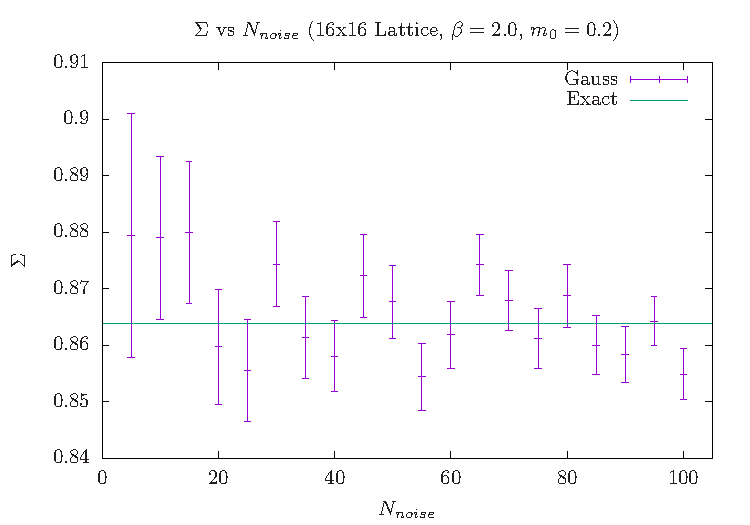
\includegraphics[width=0.8\linewidth]{images/cc_g.pdf}
              \caption{Estimate of $\Sigma$ with Gaussian vectors.}
              \label{fig:cc_g}
\end{figure}
\begin{figure}[H]
\centering
              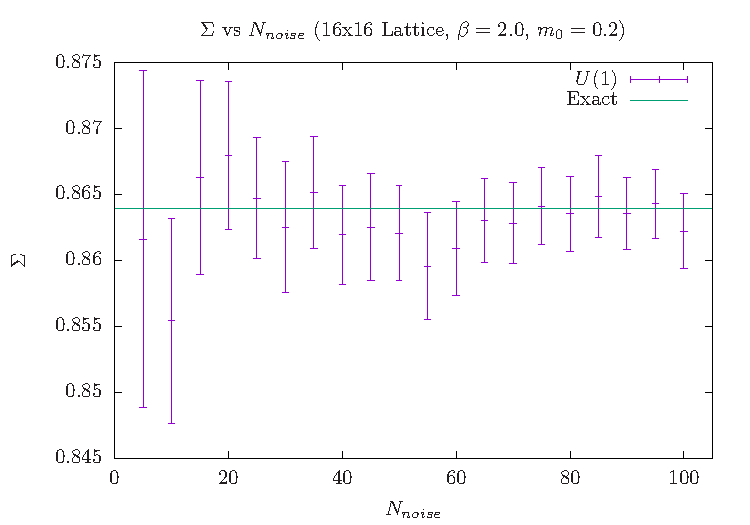
\includegraphics[width=0.8\linewidth]{images/cc_u1.pdf}
              \caption{Estimate of $\Sigma$ with $U(1)$ vectors.}
              \label{fig:cc_u1}
\end{figure}
\newpage
\begin{figure}[H]
\centering
              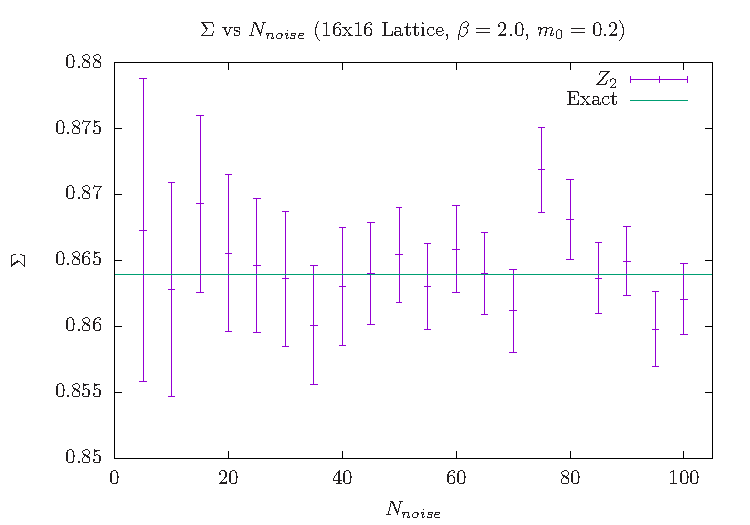
\includegraphics[width=0.8\linewidth]{images/cc_z2.pdf}
              \caption{Estimate of $\Sigma$ with $\mathbb{Z}_2$ vectors.}
              \label{fig:cc_z2}
\end{figure}
\begin{figure}[H]
\centering
              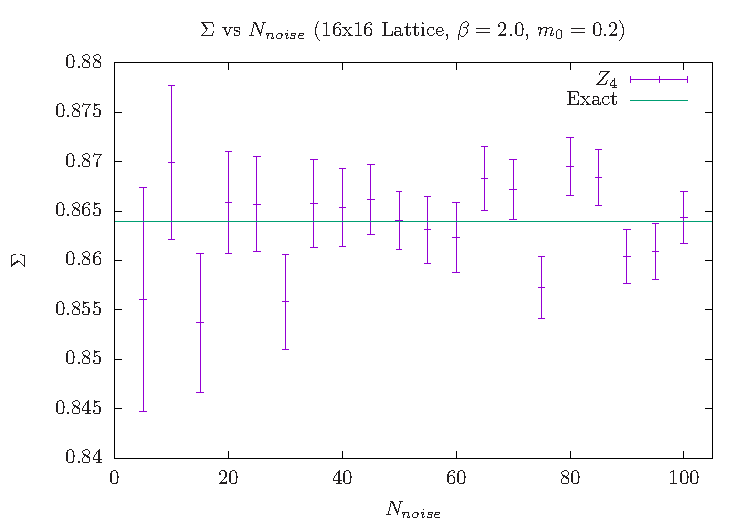
\includegraphics[width=0.8\linewidth]{images/cc_z4.pdf}
              \caption{Estimate of $\Sigma$ with $\mathbb{Z}_4$ vectors.}
              \label{fig:cc_z4}
\end{figure}
\begin{figure}[H]
    \centering
    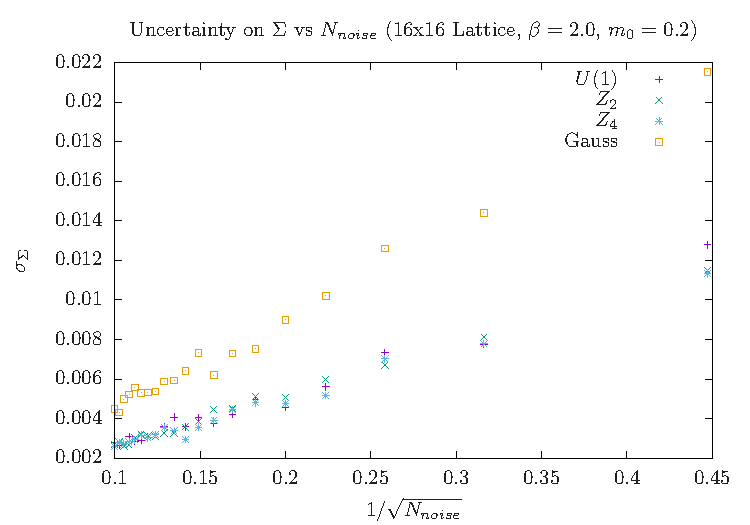
\includegraphics[width=0.8\linewidth]{images/noise_errors.pdf}
    \caption{$\sigma_\Sigma$ vs $1/\sqrt{N_{noise}}$ for each type of noise vector.}
    \label{fig:noise_errors}
\end{figure}
\begin{figure}[H]
    \centering
    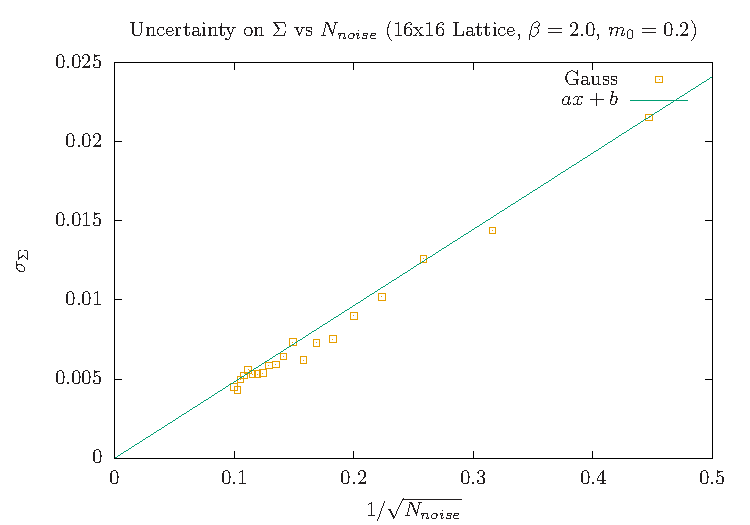
\includegraphics[width=0.8\linewidth]{images/dev_g.pdf}
    \caption{$\sigma_\Sigma$ vs $1/\sqrt{N_{noise}}$ for Gaussian noise vectors.}
    \label{fig:dev_g}
\end{figure}
\begin{figure}[H]
    \centering
    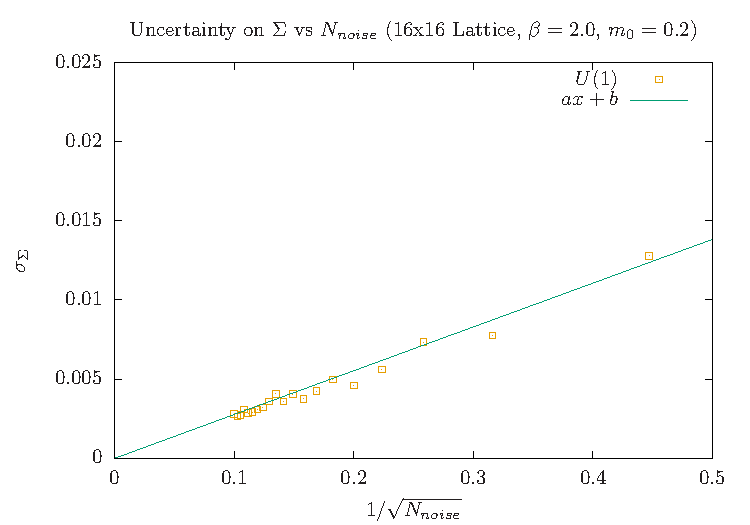
\includegraphics[width=0.8\linewidth]{images/dev_u1.pdf}
    \caption{$\sigma_\Sigma$ vs $1/\sqrt{N_{noise}}$ for $U(1)$ noise vectors.}
    \label{fig:dev_u1}
\end{figure}
\begin{figure}[H]
    \centering
    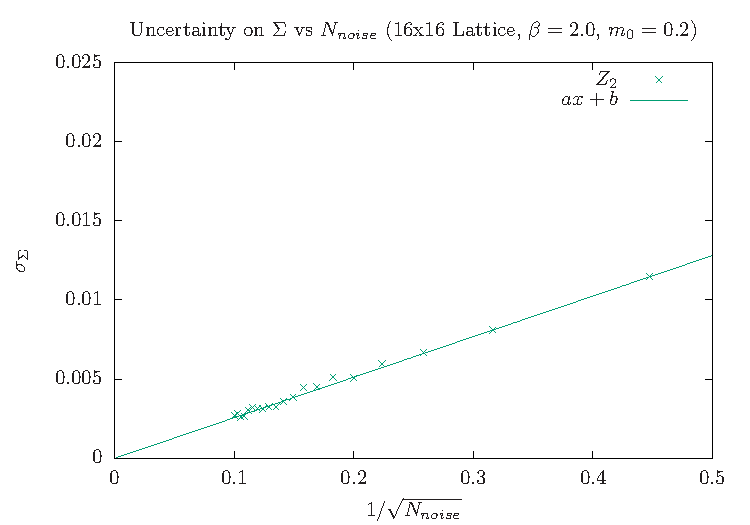
\includegraphics[width=0.8\linewidth]{images/dev_z2.pdf}
    \caption{$\sigma_\Sigma$ vs $1/\sqrt{N_{noise}}$ for $\mathbb{Z}_2$ noise vectors.}
    \label{fig:dev_z2}
\end{figure}
\begin{figure}[H]
    \centering
    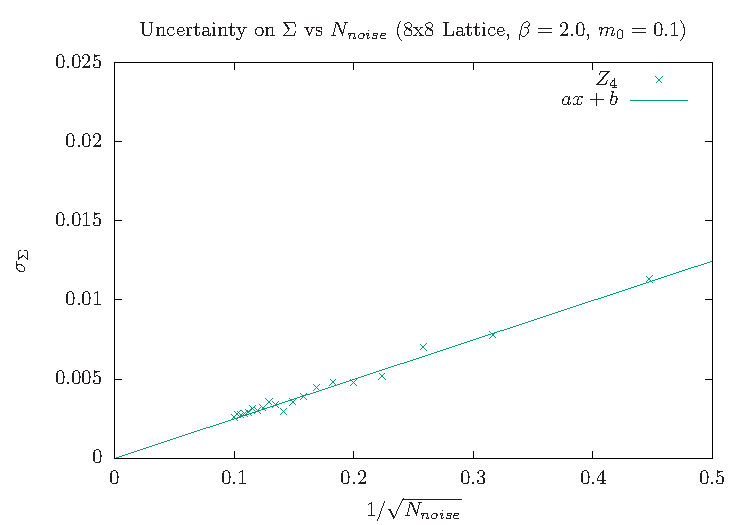
\includegraphics[width=0.8\linewidth]{images/dev_z4.pdf}
    \caption{$\sigma_\Sigma$ vs $1/\sqrt{N_{noise}}$ for $\mathbb{Z}_4$ noise vectors.}
    \label{fig:dev_z4}
\end{figure}
\newpage
\section{Hadron spectroscopy}
After this first analysis regarding some computational techniques applied in lattice computations, we can focus on the low-lying spectrum of our model and its behaviour near the chiral limit. As a first step, we will determine how to define the quark mass $m_f$ in our computations, so that we can drive it to zero in order to approach the chiral limit, where we expect our spectrum to be composed by a massless iso-triplet and a massive iso-singlet state. Consequently, we will proceed with the analysis of the scaling properties of these particles as a function of the fermion mass.
\subsection{Quark mass}
From Noether's theorem, we know that global symmetries of an action are associated with conserved currents. In lattice quantum field theories, given a global transformation of a generic field $\phi(x)$ depending on a continuous parameter $\varepsilon$ connected with the identity:
\begin{equation}
    \phi'_i(x) = \phi_i(x) + i \varepsilon \chi_i (x) 
\end{equation}
where $\chi_i(x)$ is a generic function of the fields in our theory, and the transformation leaves the action invariant:
\begin{equation}
    S[\phi_i] = S'[\phi'_i]
\end{equation}
then there exists a conserved current $J_\mu(x)$ such that, when inserted in a correlation function with an arbitrary operator $\mathcal{O}$, it satisfies:
\begin{equation}
    \langle \partial_\mu J_\mu (x) \mathcal{O}(y) \rangle = \langle \frac{\delta \mathcal{O}(y)}{\delta \phi_i(x)} \chi_i(x) \rangle
\end{equation}
and we say that the current is conserved because if $y \neq x$, then the RHS vanishes and we get an analog of $\partial_\mu J_\mu = 0$.
\\ In a QFT symmetries may be broken spontaneously or due to anomalies, for instance if the integration measure of the path integral is not invariant under the associated transformation. More generally, if the integration measure is preserved by a global transformation, we get operator relations of the form:
\begin{equation}
    \langle \delta \mathcal{O} \rangle - \langle \mathcal{O} \delta S \rangle = 0
\end{equation}
which are called Ward-Takahashi identities \cite{1950PhRv...78..182W, 1957NCim....6..371T}.
\\ The massive 2-flavour Schwinger Model with Wilson fermions is described by the action:
\begin{equation}
     S[U, \psi, \Bar{\psi}] = S_g[U] + S_F[U, \psi, \Bar{\psi}]
\end{equation}
with:
\begin{equation}
\begin{split}
    S_g[U] & = -\beta \sum_{P} \Re{U_P} \\
    S_F[\psi, \Bar{\psi}, U] & = \sum_{\substack{n, m \\ \alpha, \beta}} \Bar{\psi}_\beta(m) D_{\beta, \alpha}(m, n) \psi_\alpha(n) = \\ & = \sum_{n, \alpha} \Bar{\psi}_\alpha(n) \psi_\alpha(n) - \kappa \sum_{n, \mu} \left[ \Bar{\psi}(n)(1 - \gamma_\mu) U_\mu(n) \psi(n+\hat{\mu}) + \right. \\ & \hspace{40mm} \left. + \Bar{\psi}(n)(1 + \gamma_\mu) U_\mu^\dagger (n - \mu) \psi(m - \hat{\mu}) \right]
\end{split}
\end{equation}
The terms in $S_F$ break chiral symmetry explicitly, and the action has only the vectorial $SU(2)_V \times U(1)_V$ global symmetries. The axial $SU(2)_A \times U(1)_A$ symmetries are broken for massive fermions even for the QFT defined in the continuum, where the Ward identity associated with the axial $SU(2)_A$ generators reads:
\begin{equation}\label{continuum PCAC}
    \partial_\mu J^{\mu, a, 2} = 2 m_0 \pi^a
\end{equation}
with the definitions:
\begin{equation}
    \pi^a = \Bar{\psi} \left(\frac{\tau^a \otimes \gamma^{2}}{2}\right) \psi \hspace{10mm} J^{\mu, a, 2} = \Bar{\psi} \left(\frac{\tau^a \otimes \gamma^{\mu} \gamma^{2}}{2}\right) \psi
\end{equation}
where $\tau^a = \sigma^a$ ($a = 1, 2, 3$) are the Pauli matrices acting on flavor space, $\gamma^{\mu}$ ($\mu = 0, 1$= are the continuum equivalent of the Dirac matrices defined in \eqref{gammas}, $\gamma^2 = i\gamma^0\gamma^1$, and $\psi = (u, d)$ is a flavor-doublet.
\\ In \cite{Hip_1998} a lattice equivalent of \eqref{continuum PCAC} was derived to give a definition of the quark mass: using a pseudo-scalar source, we get the lattice PCAC-relation ($x \neq y, \mu = 0, 1$)
\begin{equation}\label{PCAC}
    \sum_\mu \left[ \langle \pi^{a \dagger} (y) J^{a}_{\mu, 2} (x) \rangle - \langle \pi^{a \dagger} (y) J^{a}_{\mu, 2} (x - \hat{\mu}) \rangle \right] = 2m \langle \pi^{a \dagger} (y) \pi^{a} (x) \rangle 
\end{equation}
with the definitions:
\begin{equation}
\begin{split}
   & \pi^a(x) = \Bar{\psi}(x) \left(\frac{\tau^a_{flavor} \otimes \gamma_{2}}{2}\right) \psi(x) \\
   & J^{a}_{\mu, 2}(x) = \frac{1}{2} \left[\Bar{\psi}(x + \hat{\mu}) U^\dagger_\mu(x) \left( \frac{\tau^a_{flavor} \otimes \gamma_\mu \gamma_2}{2} \right) \psi(x) + \Bar{\psi}(x) \left( \frac{\tau^a_{flavor} \otimes \gamma_\mu \gamma_2}{2} \right) U_\mu(x) \psi(x)\right]     
\end{split}
\end{equation}
Notice that in the exact isospin limit, i.e. $m_u = m_d$, the flavor index $a$ is irrelevant, as we get the same relation for each value of $a$, which leads to a mass degenerate iso-triplet of pions. 
\\ By inverting the previous relation, we find that the quark mass $m$ is given by:
\begin{equation}\label{mass}
    m = \frac{1}{2} \frac{\sum_\mu \left[ \langle \pi^{a \dagger} (y) J^{a}_{\mu, 2} (x) \rangle - \langle \pi^{a \dagger} (y) J^{a}_{\mu, 2} (x - \hat{\mu}) \rangle \right]}{\langle \pi^{a \dagger} (y) \pi^{a} (x) \rangle }
\end{equation}
and by computing numerically the RHS with different setups for the bare parameters, we can find the critical fermion coupling $\kappa_c(\beta)$ such that $m$ vanishes.


\subsection{Computation strategy}
Here we will briefly review how to implement the actual computation of the correlation functions mentioned above.
\\ Consider the two-point function for pions. Recall that the correlator $\langle \pi^\dagger(y) \pi(x) \rangle$ consists of a fermionic part $\langle \dots \rangle_F$ where we compute the Grassmann integrals by means of the Wick theorem, and of a gauge part where we take the average of the previous result over all gauge configuration, and so we get an estimate of the hadron propagator.
\\ For instance, if we consider a generic product of operators $C$, the correlation function will be given by:
\begin{equation}
\langle C \rangle = \langle \langle C \rangle_F \rangle_G = \frac{1}{Z} \int \mathcal{D}[U] \, e^{-S_G[U]} \mathcal{D}[\psi, \Bar{\psi}] \, e^{-S_F[{\psi, \Bar{\psi}, U]}} C[\psi, \Bar{\psi}, U]
\end{equation}
and after we carry out the integration over fermionic degrees of freedom, we get:
\begin{equation}
    \langle C \rangle = \frac{1}{Z} \int \mathcal{D}[U] \, e^{-S_G[U]} \det[D]^2 \times (\dots)_F
\end{equation}
with:
\begin{equation}
    Z = \int \mathcal{D}[U]e^{-S_G[U]} \det[D]^2
\end{equation}
where the square factor for the determinants comes from the fact that we are considering two mass-degenerate flavours, and $(\dots)_F$ labels the fermionic contractions coming from the Grassmann integration. We are left with an integral over bosonic degrees of freedom, which can be evaluated through a Monte Carlo simulation as shown in Chapter 2.
\subsubsection*{Pion correlator}
For what concerns the pion correlator, one can show that the result is independent from the flavour index $a$, if we assume exact isospin symmetry (i.e. $D_u$ = $D_d$, since the Dirac operators and propagators for the two flavors would differ only by the value of the mass parameter), and it is given by:
\begin{equation}\label{pion tp}
    \langle \pi^\dagger(y) \pi(x) \rangle = - \frac{1}{2}\tr{\gamma_2 D^{-1}(y, x) \gamma_2 D^{-1}(x, y)} = - \frac{1}{2} \sum_{\alpha, \beta} \abs{D^{-1}(x, y)_{\alpha, \beta}}^2   
\end{equation}
where $\tr(\dots)$ denotes a trace over the spinorial indices $\alpha, \beta$, and in the last step we made use of the $\gamma_2$-hermiticity property of the Dirac propagator:
\begin{equation}
    (\gamma_2)_{\alpha, \alpha'} D^{-1}(x, y)_{\alpha', \beta'}(\gamma_2)_{\beta', \beta} = D^{-1}(y, x)_{\beta, \alpha}^*
\end{equation}
The hadron correlator we are interested in is a combination of matrix elements of the quark propagator, which can be an extremely large matrix with complex entries, hence we need a convenient way to compute it and store it. Each entry $D^{-1}(x,y)_{\alpha, \beta}$ connects a quark with spinorial index $\beta$ defined at a lattice site $y$ (source) to a quark with spinorial index $\alpha$ defined at a lattice site $x$ (sink). These entries in one particular gauge configuration are highly correlated, and consequently we have a reduction of the information content stored in the whole matrix. 
\\ Operatively, one would rather fix a "site" $(\Bar{y}, \Bar{\beta})$ and consider the propagators to all the other sites of the lattice $(x, \alpha)$, which will be stored in one column of the propagator matrix:
\begin{equation}
    D^{-1}(x, \Bar{y})_{\alpha, \Bar{\beta}} = \sum_{y, \beta} D^{-1}(x, y)_{\alpha, \beta} s^{(\Bar{y}, \Bar{\beta})}(y)_{\beta}
\end{equation}
thanks to the introduction of the so-called \textit{point sources}:
\begin{equation}
    s^{(\Bar{y}, \Bar{\beta})}(y)_\beta = \delta(y - \Bar{y}) \delta_{\beta, \Bar{\beta}}
\end{equation}
which are vectors with vanishing components, except for the one associated to the lattice site $\Bar{y}$ and the Dirac index $\Bar{\beta}$, which is fixed to 1.
\\ Since the computation of correlation functions is aimed at the extrapolation of hadron masses, we want to study correlators of hadrons with zero-momentum. %Given a generic hadron interpolator $O(n_x, n_t)$, we can define a state localized on a particular time slice $n_t$ and with definite spatial momentum $p$ by taking the Fourier transform:
%\begin{equation}
%    \Tilde{O}(p, n_t) = \frac{1}{L} \sum_{n_x} O(n_x, n_t) e^{-i a n_x p}
%\end{equation}
Thus we can implement the so-called \textit{wall-to-wall propagators}, where all the points of the time slices associated with the sink and the source contribute to the same correlator:
\begin{equation}\label{C(x0 - y0)}
    C(\abs{x_0 - y_0}) = \frac{1}{L_1} \sum_{x_1, y_1} \langle \pi^\dagger(y_0, y_1) \pi(x_0, x_1) \rangle
\end{equation}
Then we exploit the translational invariance of our system to compute the contributions which concur to correlators with the same time-separation, i.e. we compute the wall-to-wall propagators between all the possible pairs of time slices $(x_0, y_0)$ with the same distance and take the average.
Operatively, this results in fixing a point source in the origin of the lattice, computing the necessary fermionic contraction (i.e. products of $D^{-1}$ matrix elements) and sweeping the fixed source over the whole lattice to repeat the process.


\subsubsection*{Pion-Current}
By means of the Wick theorem, we find that:
\begin{equation}\label{pi-j}
   \begin{split}
     \langle \pi^{a\dagger}(y) J^{a}_{\mu,2}(x) \rangle = & - \frac{1}{2} \Re{U^\dagger_\mu(x) \tr[\gamma_2 D^{-1}(y, x + \hat{\mu}) \gamma_\mu \gamma_2 D^{-1}(x, y)]} = \\
     & = \frac{1}{2} \Re{U^\dagger_\mu(x) \tr[(D^{-1}(x + \hat{\mu}, y))^* \gamma_\mu D^{-1}(x, y)]}
     \\ & = \frac{1}{2} \Re{U^\dagger_\mu(x) \sum_{\alpha, \beta} (D^{-1}(x + \hat{\mu}, y))^*_{\alpha \beta} (\gamma_\mu D^{-1}(x, y))_{\alpha \beta}}
\end{split} 
\end{equation}
The computation strategy is identical to the one embedded for the pion two-point function, but this correlator shows a little additional subtlety: on the RHS of \eqref{pi-j} we find $D^{-1}$ matrix elements defined at different time slices for $\mu = 0$, so we have to take into account the correct anti-periodic boundary conditions in the time direction. Notice also that, since we employ wall-to-wall propagators, the terms coming from $\mu = 1$ on the LHS of \eqref{PCAC} cancel out, and the only non-vanishing contributions come from the term associated to the time derivative.

\subsection{Critical coupling and critical fermion mass}
In order to study the behaviour of the low-lying spectrum of the Schwinger Model, we first need to identify an order parameter which could tell us when the chiral symmetry is expected to be restored. Using the aforementioned PCAC method, we can find the critical fermionic coupling $\kappa_c(\beta)$ at which the quark mass $m_f$ vanishes, so that we know how to approach the chiral limit with our simulations.
\\ In order to study the scaling of the fermion mass, we simulated a $16 \times 16$ lattice for different values of the bare mass $m_0$, with the coupling constant $\beta$ ranging from 1 to 6. Using \eqref{mass} we computed the mass at each possible time separation between sink and source, evaluating typically 2000-5000 configurations and embedding an adequate binning of our data to remove any autocorrelation. Each dataset has been statistically analysed via the jackknife method, so that we could give an estimate of $m_f$ at each time-separation with its error. Figure \ref{fig:mass_plateaus} shows for instance some plots produced for $\beta = 3$ at three different values of $m_0$ (or equivalently, of $\kappa = 1/(2m_0 + 4)$). From each mass plateau, through a fit to a constant, we could extrapolate the value of the quark mass for that system configuration. It is worth to notice that for systems near the chiral limit (e.g. the central mass plateau in (\ref{fig:mass_plateaus})) it has been crucial to consciously gauge the $\varepsilon_{\textrm{MD}}$ parameter which drives the time evolution. Larger values of $\varepsilon_{\textrm{MD}}$ produced indeed low acceptance rates, resulting in stiff gauge configurations, which would prevent us from taking any measurement. 
\begin{figure}[H]
    \centering
    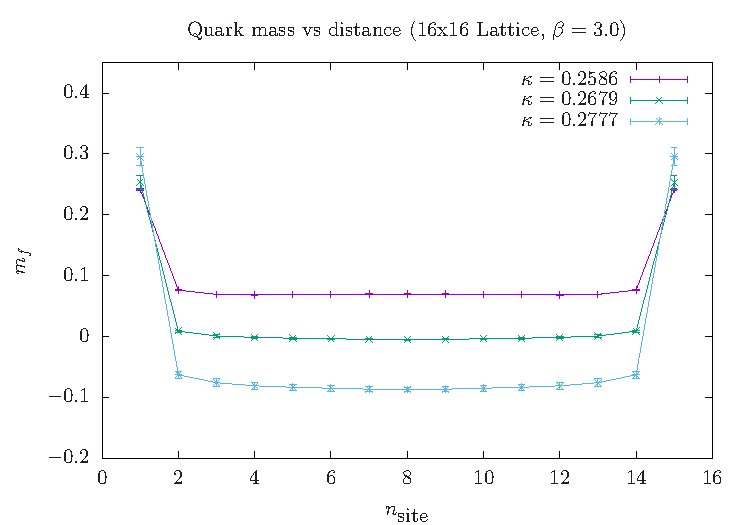
\includegraphics[width=0.7\linewidth]{images/m_corr.pdf}
    \caption{Example of mass plateau computed with \eqref{mass} for $\beta = 3$ at different values of $m_0$ (violet: $m_0 = -0.0667$, green: $m_0 = -0.1333$, blue: $m_0 = -0.2$). The lines have only been added to guide the eye.}
    \label{fig:mass_plateaus}
\end{figure}
Once that we computed $m_f$ for different values of $\kappa(\beta)$, we have been able to extrapolate the critical coupling $\kappa_c$ by performing a linear fit for each value of $\beta$. Figure (\ref{scaling mf}) shows the different measurements and the linear fits, while the estimates of $\kappa_c(\beta)$ are reported in Table \ref{tab:kc} alongside the values of the critical bare mass $m_0^{\textrm{crit}}$. Errors have been estimated from fit and properly propagated in the case of the critical bare mass, for which they are in the order of 1\%. Most measurements show an error bar smaller than the symbol itself.\footnote{Actually, the fit lines should look like filled curves with width $1\sigma$ around the central value, but errors are too small to be visible.}
\begin{figure}
    \centering
    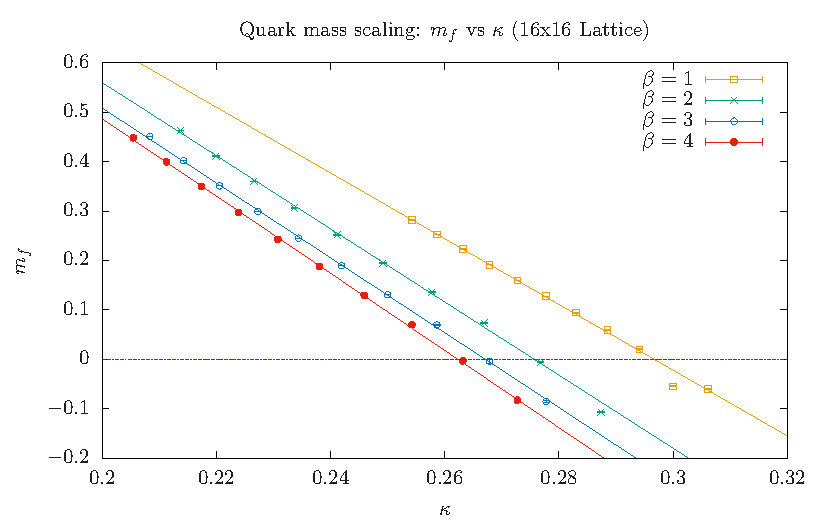
\includegraphics[width=0.8\linewidth]{images/critical.pdf}
    \caption{Scaling of the fermion mass $m_f$ vs $\kappa$ for $\beta = 1, 2, 3, 4$.}
    \label{scaling mf}
\end{figure}
\begin{table}[H]
    \centering
    \begin{tabular}{c|c|c}
      $\beta$ & $\kappa_c$ & $m_0^{\textrm{crit}}$ \\
      \hline \hline 
       1.0  & 0.2967(4) & -0.3148(21) \\
       2.0 & 0.2757(3) & -0.1864(18) \\
       3.0 & 0.2671(2) & -0.1282(10) \\
       4.0 & 0.2623(1) & -0.0939(9) \\
    \end{tabular}
    \caption{Critical coupling $\kappa_c(\beta)$ and $m_0^{\textrm{crit}}$, from fit in (\ref{scaling mf}).}
    \label{tab:kc}
\end{table}

\section{Pseudoscalar Mass}
Through the computation of the pseudoscalar two-point function expressed in Eq. \eqref{pion tp}, one can extrapolate the corresponding hadron mass, and given the similarity with the QCD$_4$ spectrum, in this section we will refer to these particles as \textit{pions} $\pi$.
From the spectral decomposition of Eq. \eqref{C(x0 - y0)}, one can show that at a time separation $n_t$ between sink and source:
\begin{equation}\label{sum spectral}
    C(n_t) = \sum_k \langle 0 | \pi | k \rangle \langle k | \pi^\dagger | 0 \rangle e^{-n_t E_k}
\end{equation}
hence if the interpolators $\pi$ couple to single particle intermediate states, the low-lying energy values $E_k$ will correspond to the hadronic masses we are looking for.
\\ In Figure \eqref{fig:pp} we show some examples of pseudoscalar correlation functions, obtained on $24 \times 24$ lattice with $\beta = 5.0$ and critical coupling $\kappa$ near the critical value. For time separations $n_t$ in the linear regions of the logarithmic plots we expect the sum in \eqref{sum spectral} to be dominated by a single exponential $\sim \exp(-n_t E_0)$, and the contributions coming from higher-energy states can be neglected.
\begin{figure}
    \centering
    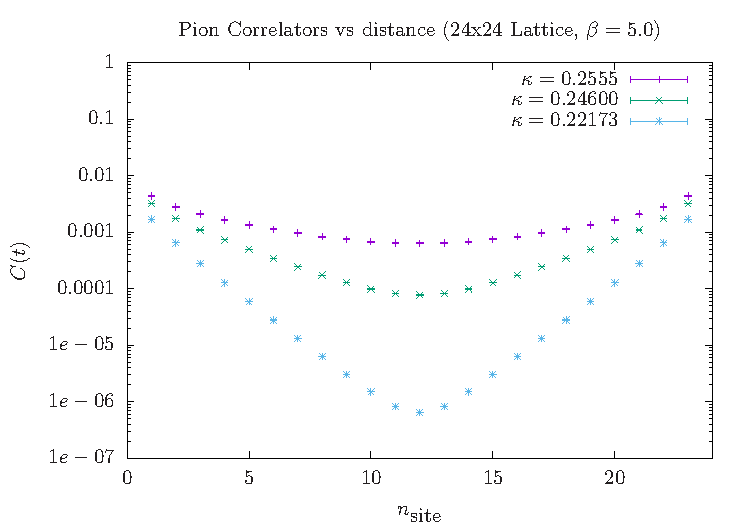
\includegraphics[width=0.7\linewidth]{images/pp.pdf}
    \caption{Pseudoscalar correlation functions at different values of $\kappa$. These are the results of simulations where we processed 4000-5000 gauge configurations.}
    \label{fig:pp}
\end{figure}
In order to extract the pseudoscalar mass $m_{\pi}$, one can define the \textit{effective pseudoscalar mass} as:
\begin{equation}
    m_\pi(n_t + 1/2) = \ln \frac{C(n_t)}{C(n_t + 1)}
\end{equation}
and once the correlator $C(n_t)$ becomes dominated by a single exponential (i.e. the ground state), the effective mass becomes constant and forms a plateau in correspondence of the lowest energy value $E_0$. Anyway, this technique may give problems around $L_0/2$, where $L_0$ is the time-extent of our lattice, therefore it is convenient to exploit the periodicity in $n_t$ of the correlation function. Indeed one can recast the previous expression in the form of:
\begin{equation}\label{meff}
    \frac{C(n_t)}{C(n_t + 1)} = \frac{\cosh(m_\pi(n_t - L_0/2)))}{\cosh(m_\pi (n_t + 1 - L_0/2))}
\end{equation}
and solve numerically for $m_\pi$ at each $n_t$, and this is how we proceeded. Equivalently, one can use:
\begin{equation}\label{meff2}
    m_\pi(n_t) = \textrm{acosh}\left(\frac{C(n_t + 1) + C(n_t - 1)}{2C(n_t)}\right)
\end{equation}
and this relation was used as a double-check on our data.
\\ As we implemented a binning method in the computation of the correlation functions, in order to extract the effective mass with its error we constructed jackknife clusters for the primary variables $C(n_t)$ at each value of $n_t$, and using \eqref{meff} we created jackknife clusters also for the effective masses, then we followed a typical jackknife data analysis. This allowed us to plot the mass plateau for the pseudoscalar correlation functions reported in Figure \eqref{fig:mass plat pions}, and though a fit to a constant we were able to extract $m_\pi$. 
\begin{figure}
    \centering
    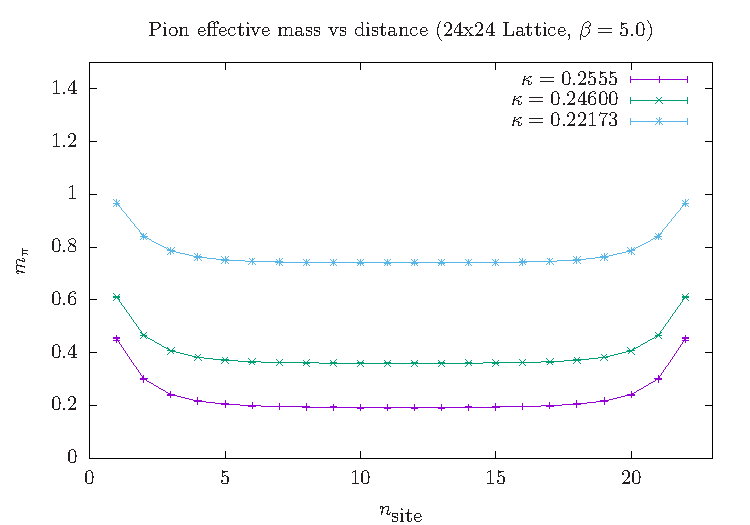
\includegraphics[width=0.7\linewidth]{images/pp_mass.pdf}
    \caption{Mass plateaus for the effective pseudoscalar mass $m_\pi$. These plots refer to the same configurations simulated in \eqref{fig:pp}. The lines were drawn only to guide the eye.}
    \label{fig:mass plat pions}
\end{figure}

\subsection{Finite size corrections}
Before we move on to the analysis of the scaling properties of iso-triplet particles, we need to take into account possible sources of systematic errors in the estimate of the pseudoscalar mass. Lattice simulations may indeed suffer from errors due to the finite size of the simulated system, therefore we need to consider some corrections for the quantities we want to compute. In Ref. \cite{Gutsfeld_1999, Luscher:1986pf} a theoretical and numerical analysis of the asymptotic finite size corrections for the pseudoscalar mass has been carried on for the Schwinger Model.
\\ Given this consideration, we reproduced a study for the scaling properties of $m_\pi$ with respect to the extent of our lattice $L$. In the aforementioned references, it is suggested to correct the pseudoscalar mass estimate accordingly to the following relation:
\begin{equation}\label{rescale}
    m_\pi(L) = m_\pi^{\infty} + A\frac{\sqrt{m_\pi^{\infty}}}{\sqrt{L}}e^{-m_{\pi}^{\infty}L}
\end{equation}
where $m_\pi^{\infty}$ labels the pion mass in the infinite volume limit, while $A$ is a numerical constant.
\begin{figure}
    \centering
    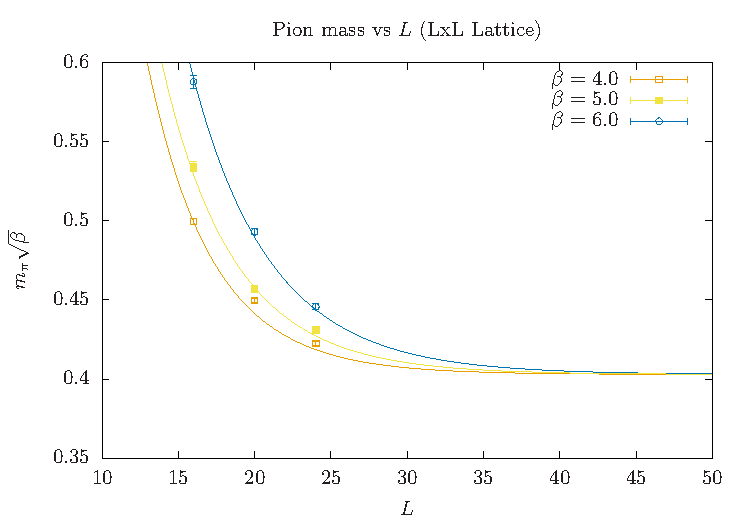
\includegraphics{images/mL.pdf}
    \caption{Scaling of $m_\pi \sqrt{\beta}$ against $L$. We plotted the values collected at $\beta = 4, 5, 6$ for $z = (m_f \sqrt{\beta})^{2/3} = 0.2$. We used three different values of $L = 16, 20, 24$. The solid lines represent fit curves obtained through Eq. \eqref{rescale}.}
    \label{fig: m vs L}
\end{figure}
In Figure \eqref{fig: m vs L} we plot the relation in Eq. \eqref{rescale} rescaled by $\sqrt{\beta}$ for various values of $\beta$. Unfortunately, we only had three available values of $L$, and a broader dataset would have helped to test the finite size effects more consistently. Anyway, our results seem to be in accordance with the aforementioned relation, and from a fit of the curves for $\beta = 4, 5, 6$ we gave an universal estimate for $A = 10.2(2)$.
\\ The measurements reported in Figure \eqref{fig: m vs L} were taken at a fixed value of the scaling parameter $z = (m_f \sqrt{\beta})^{2/3} = 0.2$, where $m_f$ is the quark mass estimated from the PCAC relation. 

\subsection{Scaling of the pseudoscalar mass}
Before we show the numerical results of our simulations, it is interesting to see some approximate calculations for $m_\pi \sqrt{\beta}$ for the massive Schwinger Model in the continuum. The first calculation was performed by Smilga in \cite{PhysRevD.55.R443}, where from a classical analysis it follows that for strong coupling and small fermion mass:
\begin{equation}\label{Smilga}
    m_\pi^{\textrm{cont}}\sqrt{\beta} \simeq 2^{5/6} e^{\gamma/3} \left(\frac{\Gamma(3/4)}{\Gamma(1/4)}\right)^{2/3} \frac{\Gamma(1/6)}{\Gamma(2/3)} (m_f \sqrt{\beta})^{2/3} = 2.008\dots (m_f \sqrt{\beta})^{2/3}
\end{equation}
where $e$ is the coupling constant of the theory, while $\gamma$ is the Eulero-Maschironi constant.
\\ On the other hand, for large masses a semi-classical analysis was performed by Gattringer in Ref. \cite{https://doi.org/10.48550/arxiv.hep-th/9503137}, where the following relation was found:
\begin{equation}\label{Gatt Cont}
     m_\pi^{\textrm{cont}}\sqrt{\beta} \simeq e^{2\gamma/3} \frac{2^{5/6}}{\pi^{1/6}} \left(m_f \sqrt{\beta}\right)^{2/3} = 2.163\dots(m_f \sqrt{\beta})^{2/3}
\end{equation}
and we can compare our non-perturbative results with this predictions.
\begin{table}
    \centering
    \begin{tabular}{c|c|c|c}
        $z$ & $\beta$ & $m_0$ & $m_{\pi}^{\infty}\sqrt{\beta}$  \\
        \hline \hline
        0.2 & 1.0 & -0.231367 & 0.398(1) \\
        0.2 & 2.0 & -0.132316 & 0.415(2) \\
        0.2 & 3.0 & -0.082626 & 0.419(3) \\
        0.2 & 4.0 & -0.057374 & 0.417(5) \\
        0.2 & 5.0 & -0.043199 & 0.425(23) \\
        0.2 & 6.0 & -0.034249 & 0.431(19) \\
        0.4 & 1.0 & -0.075308 & 0.745(1) \\
        0.4 & 2.0 & -0.017495 & 0.792(1) \\
        0.4 & 3.0 & 0.014505 & 0.805(1) \\
        0.4 & 4.0 & 0.026358 & 0.809(2) \\
        0.4 & 5.0 & 0.032526 & 0.817(3) \\
        0.4 & 6.0 & 0.036146 & 0.824(2) \\
        0.8 & 1.0 & 0.352443 & 1.357(1) \\
        0.8 & 2.0 & 0.314017 & 1.528(1) \\
        0.8 & 3.0 & 0.298677 & 1.607(1) \\
        0.8 & 4.0 & 0.276568 & 1.640(2) \\
        0.8 & 5.0 & 0.255009 & 1.653(1) \\
        0.8 & 6.0 & 0.239625 & 1.688(2) \\
    \end{tabular}
    \caption{Extrapolation of the pseudoscalar mass for a $16 \times 16$ lattice. To fix the scaling parameter $z = (m_f \sqrt{\beta})^{2/3}$, we used the suggested values of $m_0$ reported in \cite{Christian_2006} and checked using the PCAC relation. Typical statistics of the runs were 4000-5000 configurations.}
    \label{tab: pion 16}
\end{table}
\begin{table}
    \centering
    \begin{tabular}{c|c|c|c}
        $z$ & $\beta$ & $m_0$ & $m_{\pi}^{\infty}\sqrt{\beta}$  \\
        \hline \hline
        0.2 & 1.0 & -0.231367 & 0.389(1) \\
        0.2 & 2.0 & -0.132316 & 0.415(1) \\
        0.2 & 3.0 & -0.082626 & 0.420(1) \\
        0.2 & 4.0 & -0.057374 & 0.417(2) \\
        0.2 & 5.0 & -0.043199 & 0.394(3) \\
        0.2 & 6.0 & -0.034249 & 0.416(4) \\
        0.4 & 1.0 & -0.075308 & 0.746(4) \\
        0.4 & 2.0 & -0.017495 & 0.788(1) \\
        0.4 & 3.0 & 0.014505 & 0.803(1) \\
        0.4 & 4.0 & 0.026358 & 0.805(1) \\
        0.4 & 5.0 & 0.032526 & 0.816(2) \\
        0.4 & 6.0 & 0.036146 & 0.804(2) \\
        0.8 & 1.0 & 0.352443 & 1.356(1) \\
        0.8 & 2.0 & 0.314017 & 1.528(1) \\
        0.8 & 3.0 & 0.298677 & 1.602(1) \\
        0.8 & 4.0 & 0.276568 & 1.641(1) \\
        0.8 & 5.0 & 0.255009 & 1.657(1) \\
        0.8 & 6.0 & 0.239625 & 1.686(2) \\
    \end{tabular}
    \caption{Extrapolation of the pseudoscalar mass for a $20 \times 20$ lattice.}
    \label{tab: pion 20}
\end{table}
\begin{table}
    \centering
    \begin{tabular}{c|c|c|c}
        $z$ & $\beta$ & $m_0$ & $m_{\pi}^{\infty}\sqrt{\beta}$  \\
        \hline \hline
        0.2 & 1.0 & -0.231367 & 0.385(1) \\
        0.2 & 2.0 & -0.132316 & 0.407(1) \\
        0.2 & 3.0 & -0.082626 & 0.408(1) \\
        0.2 & 4.0 & -0.057374 & 0.409(2) \\
        0.2 & 5.0 & -0.043199 & 0.406(2) \\
        0.2 & 6.0 & -0.034249 & 0.407(3) \\
        0.4 & 1.0 & -0.075308 & 0.745(4) \\
        0.4 & 2.0 & -0.017495 & 0.787(1) \\
        0.4 & 3.0 & 0.014505 & 0.801(1) \\
        0.4 & 4.0 & 0.026358 & 0.805(1) \\
        0.4 & 5.0 & 0.032526 & 0.808(1) \\
        0.4 & 6.0 & 0.036146 & 0.808(1) \\
        0.8 & 1.0 & 0.352443 & 1.357(1) \\
        0.8 & 2.0 & 0.314017 & 1.527(1) \\
        0.8 & 3.0 & 0.298677 & 1.604(1) \\
        0.8 & 4.0 & 0.276568 & 1.642(1) \\
        0.8 & 5.0 & 0.255009 & 1.660(1) \\
        0.8 & 6.0 & 0.239625 & 1.679(1) \\
    \end{tabular}
    \caption{Extrapolation of the pseudoscalar mass for a $24 \times 24$ lattice.}
    \label{tab: pion 24}
\end{table}
\\ We collected values of the pseudoscalar mass for lattices of different size, namely with $L = 16, 20, 24$. The dynamical parameters have been set accordingly to the dataset produced in Ref. \cite{Christian_2006}, so that we could make a comparison of our results. Each measurement of the pseudoscalar mass has been corrected to the infinite volume value accordingly to Eq. \eqref{rescale}, and the results have been reported in Table \eqref{tab: pion 16}, Table \eqref{tab: pion 20} and Table \eqref{tab: pion 24}.
\\ We can draw the conclusion that at any value of the scaling parameter $z$, our measurements of $m_\pi^{\infty}\sqrt{\beta}$ are in good accordance with the reference results for the largest lattice, while for $L = 16$ and $L = 20$ there are more fluctuations at lower values of $z$.
\\ This may come from the fact that the spectral decomposition in \eqref{sum spectral} is dominated by the lightest state only at large distances, and clearly broader lattices allow us to explore bigger time-separations between the pseudoscalar interpolators.
\\ Nonetheless, we still were able to draw some conclusions regarding the continuum predictions mentioned before. In Figure \eqref{fig: beta z02}, \eqref{fig: beta z04} and \eqref{fig: beta z08} we plotted the scaling of $m_\pi^{\infty}\sqrt{\beta}$ against $\beta$ for $z = 0.2, 0.4$ and $0.8$, respectively, and in each plot we also draw with dashed lines the continuum predictions \eqref{Smilga} and \eqref{Gatt Cont}. 
\\ We expect the pseudoscalar mass to reach one of those values for larger $\beta$, since this parameter is linked to the lattice spacing by the relation $\beta = 1/a^2e^2$. For $z = 0.2$, we have that at larger values of $\beta$ the fermion mass becomes sufficiently small, hence we expect the pseudoscalar mass to be near the Smilga prediction \eqref{Smilga}. This behaviour is confirmed for $L = 24$, while the other datasets show large fluctuations and it is not possible to draw a definite conclusion.
\begin{figure}
    \centering
    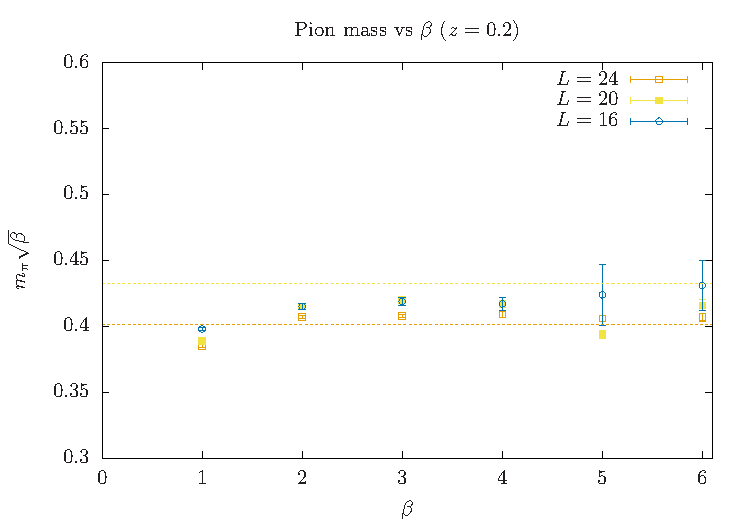
\includegraphics[width=0.8\linewidth]{images/beta02.pdf}
    \caption{Scaling of $m_\pi^{\infty}\sqrt{\beta}$ vs $\beta$ for $z = (m_f \sqrt{\beta})^{2/3} = 0.2$. Upper dashed line: continuum prediction \eqref{Smilga}, lower dashed line: continuum prediction \eqref{Gatt Cont}.}
    \label{fig: beta z02}
\end{figure}
\\ For $z = 0.4$ we have a similar outcome, and indeed the plots with $L = 24$ and $L = 20$ clearly show a drift in the scaling curves towards the classical prediction by Smilga. For $z = 0.8$ the scaling behaviour changes: the fermion mass is now further from the chiral limit, hence all the datasets seem to tend toward the semi-classical prediction \eqref{Gatt Cont}. 
\begin{figure}
    \centering
    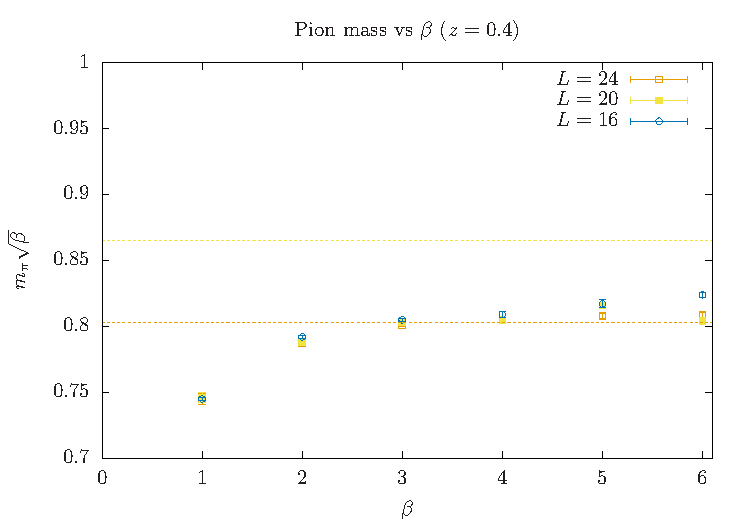
\includegraphics[width=0.8\linewidth]{images/beta04.pdf}
    \caption{Scaling of $m_\pi^{\infty}\sqrt{\beta}$ vs $\beta$ for $z = (m_f \sqrt{\beta})^{2/3} = 0.4$}
    \label{fig: beta z04}
\end{figure}
\begin{figure}
    \centering
    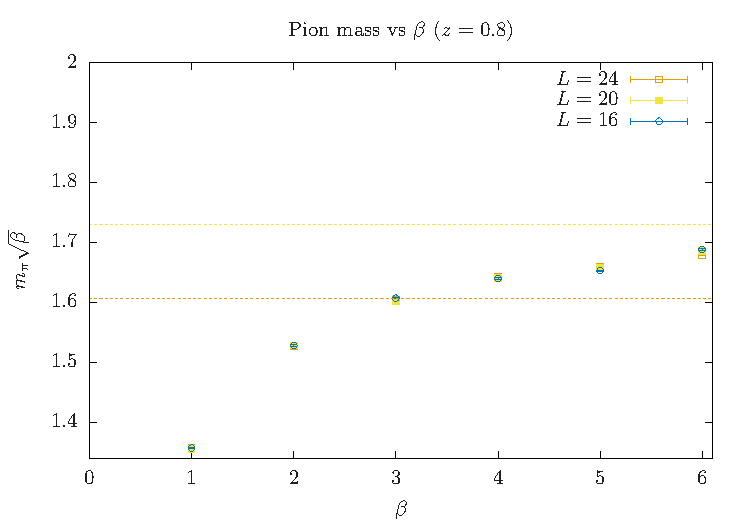
\includegraphics[width=0.8\linewidth]{images/beta08.pdf}
    \caption{Scaling of $m_\pi^{\infty}\sqrt{\beta}$ vs $\beta$ for $z = (m_f \sqrt{\beta})^{2/3} = 0.8$}
    \label{fig: beta z08}
\end{figure}
\newpage
As a final study, we can now check the scaling properties of the pseudoscalar mass with respect to the parameter $z$, in particular for what concerns its behaviour towards the chiral limit. In Figure \eqref{fig: scaling z} we report the result obtained on a $20 \times 20$ lattice for $\beta = 2$ and $4$.
The values of the quark mass $m_f$ have been computed with the PCAC relation as usual, and we did not report error bars on it as they were essentially negligible.
All the analysed pseudoscalar masses have been corrected to the infinite volume value $m_\pi^\infty$ analogously to what we did before.
\begin{figure}
    \centering
    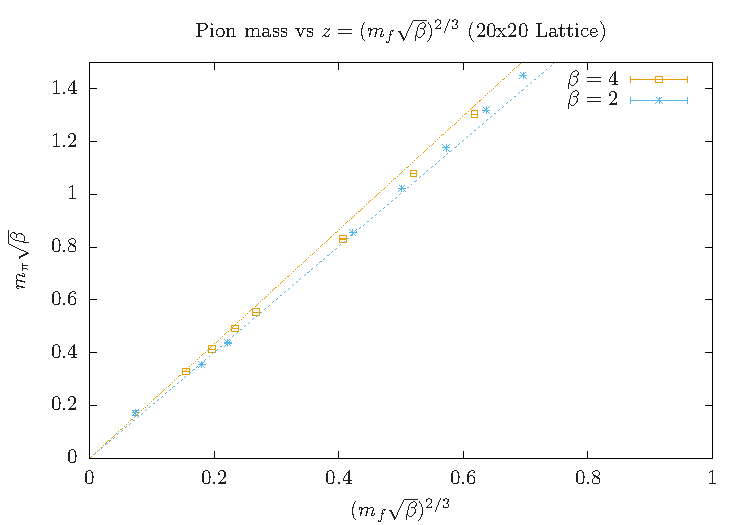
\includegraphics{images/scaling.pdf}
    \caption{Scaling of the pseudoscalar mass $m_\pi^\infty \sqrt{\beta}$ against $z$ for $\beta = 2, 4$. Upper dashed line: semi-classical continuum approximation \eqref{Gatt Cont}, lower dashed line: classical continuum approximation \eqref{Smilga}. We collected each measure studying 10000 configurations.}
    \label{fig: scaling z}
\end{figure}
The dashed lines in the plot are the continuum approximations previously defined, and the measurements seem to be coherent with these predictions. For larger values of $z$, we have higher values of the fermion mass, and $m_\pi^\infty\sqrt{\beta}$ drifts slightly more towards the semi-classical approximation. To draw more precise conclusion regarding the accordance with these relations towards the chiral limit, it would have been necessary to collect more data at lower values of $z$, but the results for $\beta = 2$ seem to be in very good accordance with the classical analytical result.
Altogether it is clear that the pseudoscalar mass tends to zero as the fermion mass vanishes, hence the approach to the chiral limit respects our prediction.
\newpage
\section{Iso-singlet state}
Now we can focus on the behaviour of the iso-singlet state, which we can call an "$\eta$-meson" in analogy with QCD$_4$. This state does not carry any flavor-index and its spinorial structure is given by:
\begin{equation}
    \eta(x) = \frac{1}{2} \Bar{\psi}(x) \left(\mathbb{1}_{flavor} \otimes \gamma_2\right) \psi(x)
\end{equation}
where as usual $\psi = (u, d)$ is a flavor-doublet and $\gamma_2 = i \gamma_0 \gamma_1$. We are interested in the computation of its two-point function $\langle \eta^\dagger(y) \eta(x) \rangle$, which takes contributions from the so-called \textit{disconnected pieces}, and these expressions require an higher computational effort with respect to the connected terms we encountered for the pion correlation function. Namely, using the Wick theorem to compute the fermionic contractions we find that:
\begin{equation}
\begin{split}
        \langle \eta^\dagger(y) \eta(x) \rangle &= \langle \tr[\gamma_2 D^{-1}(y,y)]\tr[\gamma_2 D^{-1}(x,x)] - \frac{1}{2}\tr[\gamma_2 D^{-1}(y,x) \gamma_2 D^{-1}(x,y)] \rangle \\
        &= \langle \tr[\gamma_2 D^{-1}(y,y)]\tr[\gamma_2 D^{-1}(x,x)]\rangle -\frac{1}{2} \sum_{\alpha, \beta} \abs{D^{-1}_{\alpha, \beta}(x,y)}^2
\end{split}
\end{equation}
where the second term corresponds to the pion two-point function \eqref{pion tp}, while the first term corresponds to the disconnected contributions, which are given by the combination of propagators matrix elements of the form $D^{-1}(x,x)_{\alpha, \beta}$, i.e. propagators which transport a fermion from a site $x$ back to the same site.
\\ The computation strategy for these terms is still based on the introduction of point sources, analogously to what we did for the iso-triplet states, but the computational resources needed to store all the necessary contributions are way higher. Operatively, this was sensibly visible from the fact that simulations which endowed this computation were much longer and produced results with less accuracy, given the same statistics volume.
\\ Consider for instance Figure \eqref{fig: eta corr}, which shows the correlation function of the iso-singlet state computed on a $20 \times 20$ lattice ($\beta = 2$, $\kappa = 0.21367$), and compare it with the analogous plots for the iso-triplet states \eqref{fig:pp}. The linear behaviour (on a logarithmic scale), where we expect the spectral decomposition to be dominated by a single state, is still clearly visible, but the values towards the central region are affected by large errors.
\begin{figure} 
    \centering
    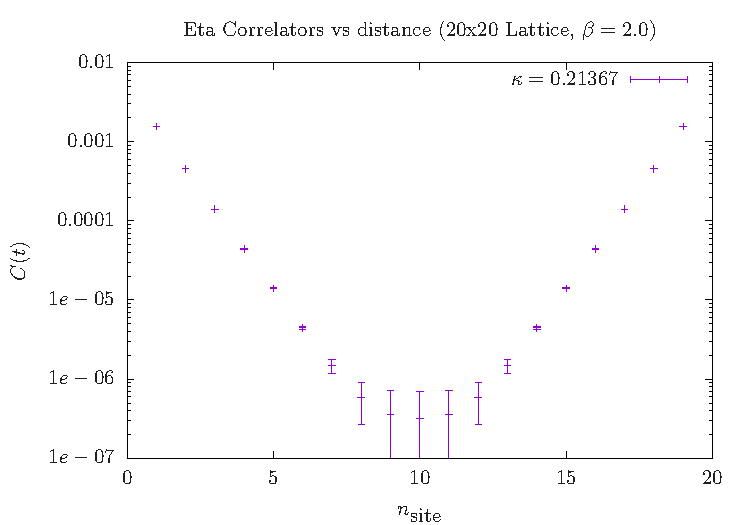
\includegraphics[width = 0.8\linewidth]{images/eta_corr.pdf}
    \caption{Correlation function for the $\eta$-meson, computed for $\beta = 2$ and $\kappa = 0.21367$. In these runs we processed 5000 gauge configurations.}
    \label{fig: eta corr}
\end{figure}
The statistical uncertainty of our measurements and the higher computational effort required to process these simulations prevented us from performing a deeper analysis for this state, similarly to what we did for the pseudoscalar mass, hence we analysed the scaling properties of the $\eta$-meson mass exploiting the results found for $m_\pi$. 

\subsection{Scaling of $m_\eta$}
The computation of $m_\eta$ was performed following the same procedure as for the pseudoscalar mass $m_\pi$, namely extrapolating the effective mass numerically with Eq. \eqref{meff} and correcting the result with the infinite volume extrapolation \eqref{rescale}.
\\ The iso-singlet state remains massive in the chiral limit, and from a semi-classical analysis it was found that for the continuum Schwinger Model $m_\eta$ is described by the relation:
\begin{equation}\label{prediction eta}
    m_\eta \sqrt{\beta} = \sqrt{\frac{2}{\pi} + \left(m_\pi \sqrt{\beta}\right)^2}
\end{equation}
hence when we reach the chiral limit and the pion mass vanishes, the mass $m_\eta$ approaches the value:
\begin{equation}
    m_\eta \sqrt{\beta} = \sqrt{\frac{2}{\pi}}
\end{equation}
In Figure \eqref{fig: scaling eta} we reported the analysis of the scaling properties of $m_\eta^{\infty}\sqrt{\beta}$ performed on a $20 \times 20$ lattice for $\beta = 2$ and $4$. The fermion mass was newly found through the PCAC relation, so that we could estimate the scaling parameter $z = (m_f \sqrt{\beta})^{2/3}$. 
\\ The dashed lines in the plot correspond to the theoretical prediction \eqref{prediction eta}, where we used the approximations \eqref{Smilga} (lower line) and \eqref{Gatt Cont} (upper line) as an input for the pion mass. The horizontal line represents the expected value for $m_\eta \sqrt{\beta}$ in the chiral limit. The correct behaviour is more evident for $\beta = 4$, since we are closer to the continuum limit, but better conclusion could be drawn by collecting more data at lower values of $z$, given the large errors and fluctuations which affect our measurements in this region.
\begin{figure}
    \centering
    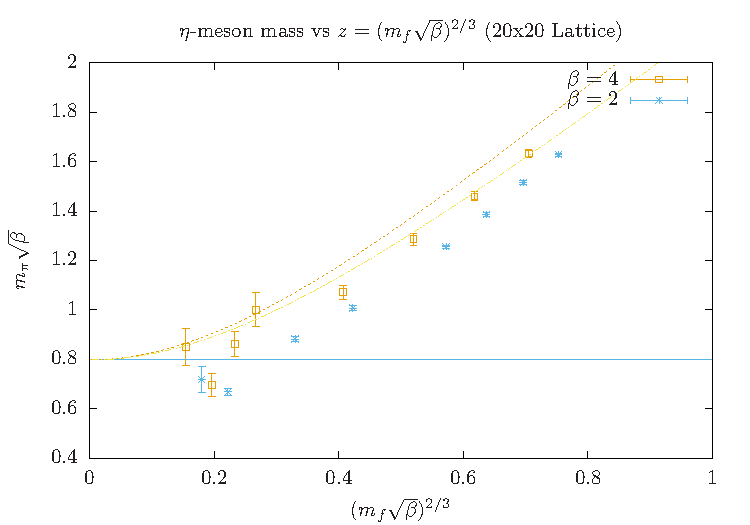
\includegraphics{images/scaling_eta.pdf}
    \caption{Scaling of $m_\eta^\infty\sqrt{\beta}$ as a function of $z = (m_f \sqrt{\beta})^{2/3}$. Upper dashed line: theoretical prediction \eqref{prediction eta} with the insertion of the semi-classical approximation \eqref{Gatt Cont} for $m_\pi\sqrt{\beta}$. Lower dashed line: theoretical prediction with the insertion of the classical approximation \eqref{Smilga}. We collected each measure studying 10000 configurations.}
    \label{fig: scaling eta}
\end{figure}
For what concerns the analytical prediction \eqref{prediction eta}, the relation describes moderately well our data for $\beta = 4$, in particular when we input Smilga's classical prediction for the pion mass. Typically, the behaviour predicted by this semi-classical analysis would be more evident at larger values of the fermion mass $m_f$, while at smaller values the quantum fluctuations become more significant, resulting in a larger deviation from the analytical formula.
\\ In conclusion, the analysis for the iso-singlet state cannot be accounted as completely satisfying, but its general behaviour towards the chiral limit seems to be reasonably described, i.e. the $\eta$-meson remains massive when the fermion mass vanishes, and its value tends to $\sqrt{2/\pi}$.
\chapter{Current factorization of the fermion determinant}
\label{chap: FactStd}
The broader goal of this work consists in the exploration of new numerical methods for lattice gauge theories, namely lattice QCD.
\\ As we have already seen, when dynamical fermions are included in lattice gauge theories, we require the Grassmann quark fields to be analytically integrated out first, causing the loss of the manifest locality of the action and of the observables (see Chap. 2.1), as the quark determinant and propagator are non-local functionals of the background gauge fields. 
 Typically, as we have explicitly done for the Schwinger Model, the resulting effective gauge theory is simulated with variants of the hybrid Monte Carlo algorithm. The urge of finding different numerical approaches comes from the fact that the standard Monte Carlo evaluation of most hadronic correlators, with some relevant exceptions (e.g. the pion two-point function), is affected by an exponential degradation of the signal-to-noise ratio (S/N) \cite{PARISI1984203,Lepage:1989hd}. Namely, the variance of a correlator decays exponentially in the time-separation between sink and source with a faster rate than the signal itself.
 \\ Throughout the years many noise-reduction ideas have been developed to tackle down this problem, for instance \textit{multilevel algorithms}, which have been applied to lattice Yang-Mills theories for a long time \cite{L_scher_2001, Meyer_2003, Della_Morte_2009, Della_Morte_2011}, where the local building blocks of the observables are computed independently, so that the degradation of the S/N is avoided.
 \\ Multilevel algorithms in theories with dynamical fermions are more complicated to implement, due to the non-localities mentioned above. To make these techniques feasible, over the last two decades there have been several attempts to rewrite the fermion determinant through a local bosonic field theory. 
 The main ingredients are a factorization of the gauge-field dependence of the quark determinant in lattice QCD with Wilson fermions, based on the domain decomposition of the lattice \cite{L_scher_2004, L_scher_2005, C__2016, C__2017, Giusti_2022}, and the introduction of multi-boson auxiliary fields living on the boundaries of the aforementioned domains \cite{L_scher_1994}. This combination leads to a bosonic action which is local in the block gauge, pseudofermion and multi-boson fields, and together with the factorization of fermionic observables \cite{C__2016} it makes it feasible to conduce multilevel simulations in lattice QCD.
 \\ Many numerical tests have been performed (e.g. \cite{Giusti_2018, Dalla_Brida_2021}), and in this chapter we will review the factorization of the quark determinant presented in \cite{C__2017}. In this work the lattice gets decomposed in overlapping domains along one dimension only, although lately it has been proposed a four-dimensional generalization of this technique \cite{Giusti_2022}. From numerical experience, we can conjecture that contributions which depend on gauge fields living in different regions are suppressed exponentially in the time-separation between sink and source \cite{C__2016}, hence we can control the magnitude of such contributions by tuning the thickness of the overlapping region between the domains of interest.

 \section{Block decomposition of the determinant}

 The goal of this process consists in the decomposition of the effective fermion action in contributions which depend only on the local block gauge, pseudofermion and multiboson fields.
 Consider a non-overlapping 3-block decomposition of the lattice, where each block $\Lambda_i$ $(i = 0, 1, 2)$ may be the union of disconnected regions, but we require that the Dirac operator cannot connect points from $\Lambda_0$ and $\Lambda_2$. Without loss of generality, we can implement periodic and open boundary conditions in the spatial and temporal directions, respectively. Minor adjustements are required to implement periodic boundary conditions in the time direction. Figure \eqref{fig: Decomp} depicts this decomposition in three thick time slices $\Lambda_i$. 
 \begin{figure}
     \centering


\tikzset{every picture/.style={line width=0.75pt}} %set default line width to 0.75pt        

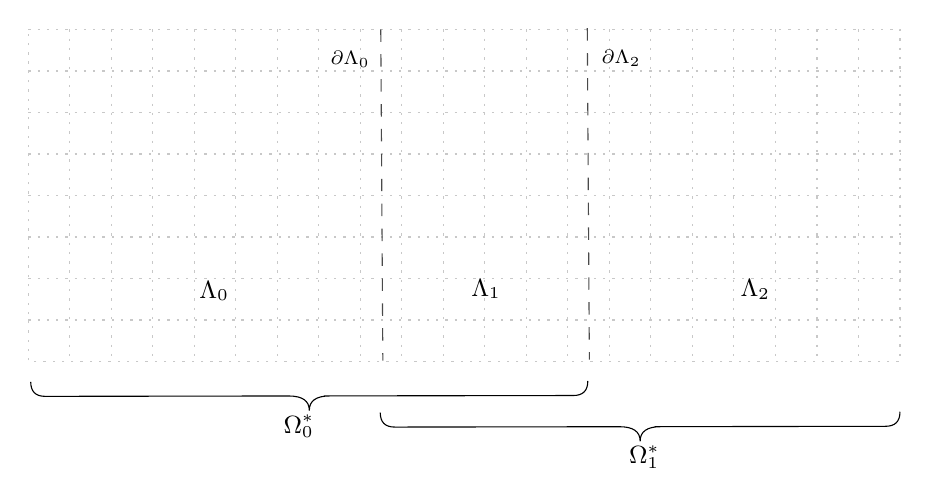
\begin{tikzpicture}[x=0.75pt,y=0.75pt,yscale=-1,xscale=1]
%uncomment if require: \path (0,300); %set diagram left start at 0, and has height of 300

%Shape: Grid [id:dp36732851129859456] 
\draw  [draw opacity=0][dash pattern={on 0.84pt off 2.51pt}] (110.18,50.67) -- (530.18,50.67) -- (530.18,210.67) -- (110.18,210.67) -- cycle ; \draw  [color={rgb, 255:red, 200; green, 200; blue, 200 }  ,draw opacity=1 ][dash pattern={on 0.84pt off 2.51pt}] (130.18,50.67) -- (130.18,210.67)(150.18,50.67) -- (150.18,210.67)(170.18,50.67) -- (170.18,210.67)(190.18,50.67) -- (190.18,210.67)(210.18,50.67) -- (210.18,210.67)(230.18,50.67) -- (230.18,210.67)(250.18,50.67) -- (250.18,210.67)(270.18,50.67) -- (270.18,210.67)(290.18,50.67) -- (290.18,210.67)(310.18,50.67) -- (310.18,210.67)(330.18,50.67) -- (330.18,210.67)(350.18,50.67) -- (350.18,210.67)(370.18,50.67) -- (370.18,210.67)(390.18,50.67) -- (390.18,210.67)(410.18,50.67) -- (410.18,210.67)(430.18,50.67) -- (430.18,210.67)(450.18,50.67) -- (450.18,210.67)(470.18,50.67) -- (470.18,210.67)(490.18,50.67) -- (490.18,210.67)(510.18,50.67) -- (510.18,210.67) ; \draw  [color={rgb, 255:red, 200; green, 200; blue, 200 }  ,draw opacity=1 ][dash pattern={on 0.84pt off 2.51pt}] (110.18,70.67) -- (530.18,70.67)(110.18,90.67) -- (530.18,90.67)(110.18,110.67) -- (530.18,110.67)(110.18,130.67) -- (530.18,130.67)(110.18,150.67) -- (530.18,150.67)(110.18,170.67) -- (530.18,170.67)(110.18,190.67) -- (530.18,190.67) ; \draw  [color={rgb, 255:red, 200; green, 200; blue, 200 }  ,draw opacity=1 ][dash pattern={on 0.84pt off 2.51pt}] (110.18,50.67) -- (530.18,50.67) -- (530.18,210.67) -- (110.18,210.67) -- cycle ;
%Straight Lines [id:da8151691865200523] 
\draw [color={rgb, 255:red, 74; green, 74; blue, 74 }  ,draw opacity=1 ] [dash pattern={on 4.5pt off 4.5pt}]  (280.03,50.61) -- (281.03,210.28) ;
%Straight Lines [id:da2624795881970642] 
\draw [color={rgb, 255:red, 74; green, 74; blue, 74 }  ,draw opacity=1 ] [dash pattern={on 4.5pt off 4.5pt}]  (379.53,50.08) -- (380.53,209.75) ;
%Shape: Brace [id:dp41866974630216447] 
\draw   (111.38,220.45) .. controls (111.39,225.12) and (113.72,227.45) .. (118.39,227.44) -- (235.59,227.26) .. controls (242.26,227.25) and (245.59,229.57) .. (245.6,234.24) .. controls (245.59,229.57) and (248.92,227.24) .. (255.59,227.23)(252.59,227.23) -- (372.79,227.04) .. controls (377.46,227.03) and (379.79,224.7) .. (379.78,220.03) ;
%Shape: Brace [id:dp9584637663157783] 
\draw   (279.78,235.25) .. controls (279.79,239.92) and (282.12,242.25) .. (286.79,242.24) -- (394.99,242.07) .. controls (401.66,242.06) and (404.99,244.39) .. (405,249.06) .. controls (404.99,244.39) and (408.32,242.05) .. (414.99,242.04)(411.99,242.05) -- (523.19,241.87) .. controls (527.86,241.86) and (530.19,239.53) .. (530.18,234.86) ;

% Text Node
\draw (231.99,235.07) node [anchor=north west][inner sep=0.75pt]  [font=\small]  {$\Omega _{0}^{*}$};
% Text Node
\draw (398.39,249.87) node [anchor=north west][inner sep=0.75pt]  [font=\small]  {$\Omega _{1}^{*}$};
% Text Node
\draw (191.43,170.7) node [anchor=north west][inner sep=0.75pt]  [font=\small]  {$\Lambda _{0}$};
% Text Node
\draw (322.43,169.7) node [anchor=north west][inner sep=0.75pt]  [font=\small]  {$\Lambda _{1}$};
% Text Node
\draw (452.18,170.07) node [anchor=north west][inner sep=0.75pt]  [font=\small]  {$\Lambda _{2}$};
% Text Node
\draw (254.63,59.7) node [anchor=north west][inner sep=0.75pt]  [font=\scriptsize]  {$\partial \Lambda _{0}$};
% Text Node
\draw (385.23,59.5) node [anchor=north west][inner sep=0.75pt]  [font=\scriptsize]  {$\partial \Lambda _{2}$};


\end{tikzpicture}

     \caption{Decomposition of the lattice in three thick time slices.}
     \label{fig: Decomp}
 \end{figure}
 \\ Given this domain-decomposition, we can write the hermitian $\mathcal{O}(a)$-improved massive Dirac operator $Q = \gamma_5 D$ (see Appendix \ref{app: Wilson improved op}) in a block form\footnote{For a broader view on the block terminology and decomposition, see Ref. \cite{C__2017}. To keep the
notation compact, a block matrix $Q_{\Lambda_{i,j}}$ denotes either a single block of the whole quark matrix, or the full matrix
with just that block different from zero.}:
 \begin{equation}\label{Q}
    Q = \begin{pmatrix}
 Q_{\Lambda_{0,0}} & Q_{\Lambda_{0,1}} & 0  \\
   Q_{\Lambda_{1,0}} & Q_{\Lambda_{1,1}} & Q_{\Lambda_{1,2}} \\
   0 & Q_{\Lambda_{2,1}} & Q_{\Lambda_{2,2}} \\
\end{pmatrix}
\end{equation}
Since we will refer frequently to quark fields which live in a particular block, it is convenient to define projector operators:
\begin{equation}
    [P_{\Lambda_i}\psi](x) = \left\{ \begin{array}{rcl} \psi(x) \hspace{3mm} \mbox{if} \hspace{2mm} x \in \Lambda_i \\ 0  \hspace{3mm} \mbox{elsewhere}  \\ \end{array} \right.
\end{equation}
which act on subspaces of fermion fields with support in the domain $\Lambda_i$. \\ Analogously, we can define projectors associated with quark fields living on inner and outer boundaries of each domain, namely $P_{\partial \Lambda_i}$ and $P_{\partial \Lambda_i^*}$. We define the inner boundary of a block to be the set of points at a unitary distance from the previous and the following block, and these projectors satisfy the relation:
\begin{equation}
    P_{\partial \Lambda_i} Q_{\Lambda_{i, j}} = Q_{\Lambda_{i, j}} P_{\partial \Lambda_j} = Q_{\Lambda_{i,j}} \hspace{5mm} i \neq j
\end{equation}
Notice that $P_{\Lambda_i}$ labels the corresponding projector independently from the dimensionality of the space where it acts on.
\\ Since we will employ a two-block partitioning of the lattice, let us define the two block operators:
\begin{equation}
    Q_{\Omega_i^*} = \begin{pmatrix}
 Q_{\Lambda_{i,i}} & Q_{\Lambda_{i,i+1}} \\
   Q_{\Lambda_{i+1,i}} & Q_{\Lambda_{i+1,i+1}} \\
\end{pmatrix}
\end{equation}
where $\Omega_i^* = \Lambda_i \cup \Lambda_{i+1}$ and $i = 0, 1$. The factorization of the determinant of $Q$ is realized as follows.
\\ Consider the partitions $\Gamma = \Lambda_0 \cup \Lambda_2$ and $\Gamma^* = \Lambda_1$. Using the Schur decomposition \eqref{Schur} on $Q$ we can write:
\begin{equation}\label{det Q}
    \det Q = \det Q_{\Lambda_{1,1}} \det S_{\Gamma} = \det Q_{\Lambda_{1,1}} \det \begin{pmatrix}
        Q_{\Lambda_{0,0}} - Q_{\Lambda_{0,1}}Q^{-1}_{\Lambda_{1,1}}Q_{\Lambda_{1,0}} & - Q_{\Lambda_{0,1}}Q^{-1}_{\Lambda_{1,1}}Q_{\Lambda_{1,2}} \\
        \\
        - Q_{\Lambda_{2,1}}Q^{-1}_{\Lambda_{1,1}}Q_{\Lambda_{1,0}} & Q_{\Lambda_{2,2}} - Q_{\Lambda_{2,1}}Q^{-1}_{\Lambda_{1,1}}Q_{\Lambda_{1,2}} \\ 
    \end{pmatrix}
\end{equation}
where $S_\Gamma$ is the Schur complement associated with $\Gamma.$ Since the inverse of the Schur complement of a matrix coincides with the matrix inverse if the latter acts upon fields defined in the same block, we can notice that:
\begin{equation}
    \begin{split}
        P_{\Lambda_0} Q^{-1}_{\Omega^*_0} P_{\Lambda_0} = S_{\Omega^*_0}^{-1} = \left[ Q_{\Lambda_{0,0}} - Q_{\Lambda_{0,1}}Q^{-1}_{\Lambda_{1,1}}Q_{\Lambda_{1,0}}  \right]^{-1} \\
        P_{\Lambda_2} Q^{-1}_{\Omega^*_1} P_{\Lambda_2} = S_{\Omega^*_1}^{-1} = \left[ Q_{\Lambda_{2,2}} - Q_{\Lambda_{2,1}}Q^{-1}_{\Lambda_{1,1}}Q_{\Lambda_{1,2}}  \right]^{-1} \\
    \end{split}
\end{equation}
For instance, we can conjecture that if we consider two points $x, y \in \Lambda_0$, then $Q^{-1}(x,y)$ is going to be well approximated by $Q_{\Omega_0^*}^{-1}$, up to corrections suppressed exponentially as $\sim\exp(-M_{\pi} \Delta)$, where $M_\pi$ is the pion mass and $\Delta$ is the thickness of the central block $\Lambda_1$ (see Ref. \cite{C__2016}). Then one can use Eq. \eqref{schur det} on \eqref{det Q} to recast it as:
\begin{equation}
    \det Q = \frac{1}{\det Q_{\Lambda_{1,1}}^{-1} \det \left[ P_{\Lambda_0} Q^{-1}_{\Omega^*_0} P_{\Lambda_0} \right] \det \left[ P_{\Lambda_2} Q^{-1}_{\Omega^*_1} P_{\Lambda_2}  \right] } \det \begin{pmatrix}
        1 & P_{\Lambda_0 Q_{\Omega^*_{0}}^{-1} Q_{\Lambda_{1,2}}} \\ 
        P_{\Lambda_2} Q_{\Omega_1^*}^{-1} Q_{\Lambda_{1,0}} & 1 \\
    \end{pmatrix}
\end{equation}
Finally, using again Eq. \eqref{Schur}, we can rewrite the last determinant of the previous expression as the determinant of a matrix acting on one of the boundaries only:
\begin{equation}\label{final det}
    \det \begin{pmatrix}
        1 & P_{\Lambda_0 Q_{\Omega^*_{0}}^{-1} Q_{\Lambda_{1,2}}} \\ 
        P_{\Lambda_2} Q_{\Omega_1^*}^{-1} Q_{\Lambda_{1,0}} & 1 \\
    \end{pmatrix} = \det \left(1 - P_{\partial \Lambda_0} Q_{\Omega_0^*}^{-1} Q_{\Lambda_{1,2}} P_{\partial \Lambda_2} Q_{\Omega_1^{*}}^{-1} Q_{\Lambda_{1,0}} P_{\partial \Lambda_0} \right)
\end{equation}
If we call:
\begin{equation}\label{w}
  w =  P_{\partial \Lambda_0} Q_{\Omega_0^*}^{-1} Q_{\Lambda_{1,2}} P_{\partial \Lambda_2} Q_{\Omega_1^{*}}^{-1} Q_{\Lambda_{1,0}} P_{\partial \Lambda_0}
\end{equation}
we can write the factorized formula for the Dirac-Wilson operator determinant:
\begin{equation}\label{det Q}
    \det Q = \frac{1}{\det Q_{\Lambda_{1,1}}^{-1} \det \left[ P_{\Lambda_0} Q^{-1}_{\Omega^*_0} P_{\Lambda_0} \right] \det \left[ P_{\Lambda_2} Q^{-1}_{\Omega^*_1} P_{\Lambda_2}  \right] } \det (1 - w)
\end{equation}
Indeed we have that:
\begin{itemize}
    \item $\det Q_{\Lambda_{1,1}}^{-1}$ depends only on the gauge fields in $\Lambda_1$;
    \item $\left[ P_{\Lambda_0} Q^{-1}_{\Omega^*_0} P_{\Lambda_0} \right]$ depends only on the gauge fields in $\Lambda_0 \cup \Lambda_1$;
    \item $\left[ P_{\Lambda_2} Q^{-1}_{\Omega^*_1} P_{\Lambda_2}  \right]$ depends only on the gauge fields in $\Lambda_1 \cup \Lambda_2$;
    \item $\det (1 - w)$ is a small correction, and it is a function of links defined across the whole lattice. Notice that this determinant is real, since all the other terms in \eqref{det Q} are.
\end{itemize}
Now we should shed more light on the magnitude of $\det(1 - w)$, in order to verify the goodness of this factorization.

\subsection{Magnitude of $w$}
In order to better understand the contribution brought by $w$, it is convenient to recast this matrix in terms of the full propagator $Q^{-1}$.
If we consider two different partitions of the lattice, namely $\Lambda_0 \cup \Lambda_1 + \Lambda_2$ and $\Lambda_0 + \Lambda_1 \cup \Lambda_2$, it is possible to show that:
\begin{equation}\label{boundary prop}
    \begin{split}
        P_{\Lambda_0} Q^{-1}_{\Omega^*_0} Q_{\Lambda_{1,2}} = P_{\partial \Lambda_0} Q^{-1} \{Q_{\Lambda_{1,2}} + Q_{\Lambda_{2,1}} Q_{\Omega_0^*}^{-1} Q_{\Lambda_{1,2}} \} \\ 
         P_{\Lambda_2} Q^{-1}_{\Omega^*_1} Q_{\Lambda_{1,0}} = P_{\partial \Lambda_2} Q^{-1} \{Q_{\Lambda_{1,0}} + Q_{\Lambda_{0,1}} Q_{\Omega_1^*}^{-1} Q_{\Lambda_{1,0}}\}
    \end{split}
\end{equation}
hence in the definition of $w$ we have two propagators between the boundaries of the blocks $\Lambda_0$ and $\Lambda_2$, each one multiplied by an effective boundary operator. A visual representation of $w$ is given in Figure \eqref{fig: op w}.
\begin{figure}
    \centering


\tikzset{every picture/.style={line width=0.75pt}} %set default line width to 0.75pt        

\begin{tikzpicture}[x=0.75pt,y=0.75pt,yscale=-1,xscale=1]
%uncomment if require: \path (0,300); %set diagram left start at 0, and has height of 300

%Shape: Grid [id:dp36732851129859456] 
\draw  [draw opacity=0][dash pattern={on 0.84pt off 2.51pt}] (110.18,50.67) -- (530.18,50.67) -- (530.18,210.67) -- (110.18,210.67) -- cycle ; \draw  [color={rgb, 255:red, 200; green, 200; blue, 200 }  ,draw opacity=1 ][dash pattern={on 0.84pt off 2.51pt}] (130.18,50.67) -- (130.18,210.67)(150.18,50.67) -- (150.18,210.67)(170.18,50.67) -- (170.18,210.67)(190.18,50.67) -- (190.18,210.67)(210.18,50.67) -- (210.18,210.67)(230.18,50.67) -- (230.18,210.67)(250.18,50.67) -- (250.18,210.67)(270.18,50.67) -- (270.18,210.67)(290.18,50.67) -- (290.18,210.67)(310.18,50.67) -- (310.18,210.67)(330.18,50.67) -- (330.18,210.67)(350.18,50.67) -- (350.18,210.67)(370.18,50.67) -- (370.18,210.67)(390.18,50.67) -- (390.18,210.67)(410.18,50.67) -- (410.18,210.67)(430.18,50.67) -- (430.18,210.67)(450.18,50.67) -- (450.18,210.67)(470.18,50.67) -- (470.18,210.67)(490.18,50.67) -- (490.18,210.67)(510.18,50.67) -- (510.18,210.67) ; \draw  [color={rgb, 255:red, 200; green, 200; blue, 200 }  ,draw opacity=1 ][dash pattern={on 0.84pt off 2.51pt}] (110.18,70.67) -- (530.18,70.67)(110.18,90.67) -- (530.18,90.67)(110.18,110.67) -- (530.18,110.67)(110.18,130.67) -- (530.18,130.67)(110.18,150.67) -- (530.18,150.67)(110.18,170.67) -- (530.18,170.67)(110.18,190.67) -- (530.18,190.67) ; \draw  [color={rgb, 255:red, 200; green, 200; blue, 200 }  ,draw opacity=1 ][dash pattern={on 0.84pt off 2.51pt}] (110.18,50.67) -- (530.18,50.67) -- (530.18,210.67) -- (110.18,210.67) -- cycle ;
%Straight Lines [id:da8151691865200523] 
\draw [color={rgb, 255:red, 74; green, 74; blue, 74 }  ,draw opacity=1 ] [dash pattern={on 4.5pt off 4.5pt}]  (280.03,50.61) -- (281.03,210.28) ;
%Straight Lines [id:da2624795881970642] 
\draw [color={rgb, 255:red, 74; green, 74; blue, 74 }  ,draw opacity=1 ] [dash pattern={on 4.5pt off 4.5pt}]  (379.53,50.08) -- (380.53,209.75) ;
%Straight Lines [id:da6638407323679787] 
\draw    (250.18,170.67) -- (410.18,170.67) ;
%Curve Lines [id:da08584860303537212] 
\draw    (410.18,110.67) .. controls (433.55,110.54) and (443.27,130.84) .. (439.33,147.86) .. controls (436.52,159.97) and (426.81,170.41) .. (410.18,170.67) ;
%Straight Lines [id:da2105866998964242] 
\draw    (250.18,110.67) -- (410.18,110.67) ;

% Text Node
\draw (405.2,163.92) node [anchor=north west][inner sep=0.75pt]  [font=\LARGE,rotate=-359.89]  {$\cdot $};
% Text Node
\draw (245.8,104.42) node [anchor=north west][inner sep=0.75pt]  [font=\LARGE,rotate=-359.89]  {$\cdot $};


\end{tikzpicture}

    \caption{Representation of the operator $w$, which acts on a single boundary and can be written as the composition of two propagators between $\partial\Lambda_0$ and $\partial \Lambda_2$. The black lines are full propagators, while the thick dots are insertions of the effective hops; see Eq. \eqref{boundary prop}.}
    \label{fig: op w}
\end{figure}
\\ We conjecture from numerical experience (see Ref. \cite{C__2016}), that if the thickness of the central block $\Delta$ is large enough, each of these propagators will decay exponentially as $\sim \exp(-\frac{1}{2} M_\pi \Delta)$, hence the norm of $w$ will be suppressed $\sim \exp(-M_\pi \Delta)$.

\subsection{Spectrum of $w$}
In order to pair the domain decomposition with the multiboson approach, we need to know more in depth the spectrum of $(1 - w)$.
\\ Given the definition of $w$ in Eq. \eqref{w} and the relation in \eqref{matrix inverse}, we can rewrite $w$ as the product of two Hermitian matrices acting upon $\partial \Lambda_0$, i.e. the inner boundary of $\Lambda_0$:
\begin{equation}
    w = \left[P_{\partial\Lambda_0} Q^{-1}_{\Omega^*_0} P_{\partial\Lambda_0}\right] \cdot \left[ Q_{\Lambda_{0,1}} Q_{\Lambda_{1,1}}^{-1} Q_{\Lambda_{1,2}} Q^{-1}_{\Omega^*_1} Q_{\Lambda_{2,1}} Q_{\Lambda_{1,1}}^{-1} Q_{\Lambda_{1,0}} \right]
\end{equation}
and this allows us to conclude that $w$ is similar to $w^{\dagger}$ (see Ref. \cite{10.2307/2042048}). This in turn implies that the characteristic polynomial of $w$ has real coefficients, and its complex eigenvalues $\delta_i$ come in conjugate pairs. This results in a symmetric spectrum with respect to the real axis, hence the determinant of $(1 - w)$ is real. Since the norm of $w$ is suppressed as $\sim \exp(-M_\pi \Delta)$, we expect the modulus of the eigenvalues $\abs{\delta_i}$ to have the same behaviour.
\\ This leads us to the conclusion that, for a suitably chosen value of $\Delta$, all the eigenvalues of $w$ satisfy $\abs{\delta_i} \ll 1$, resulting in a large spectral gap for $(1 - w)$.
 Consequently, we can express $\det(1-w)$ through an adequate polynomial approximation of $(1 - w)^{-1}.$

 \section{Multiboson factorization}
 The main result of the previous section was the factorization of the quark determinant into terms which depend only on gauge fields in the neighboring thick time slices, resulting from a non-overlapping domain decomposition. The factorization is not complete, as the term $\det(1-w)$ still depends on the link variables defined across the whole lattice, but with a suitable fine tuning of the central block thickness $\Delta$, we can treat this term as a small contribution and express it through a polynomial approximation.
 \subsection{Polynomial approximation}
 Lüscher's original multiboson idea \cite{L_scher_1994} can be generalized to complex matrices \cite{Bori_i_1995, Bori_i_1996, Jegerlehner_1996}, hence the first step we need to take into account is the approximation of the function $1/z$ (with $z \in \mathbb{C}$) via the polynomial:
 \begin{equation}\label{pol}
    P_N (z) \equiv \frac{1 - R_{N+1}(z)}{z} = c_N \prod_{k = 1}^N (z - z_k)
 \end{equation}
 where $N$ is chosen to be even, and the $N$ roots of $P_N(z)$ are obtained by requiring that for the remainder, which is defined in \eqref{remainder}, $R_{N+1}(0) = 1$. The roots $z_k$ of $P_N(z)$ can be chosen to lie on an ellipse passing through the origin of the complex plane with center $1$ and foci $1 \pm c$, hence from \eqref{roots}:
 \begin{equation}
     u_k = 1 - z_k = \cos(\frac{2\pi k}{N+1}) + i \sqrt{1 - c^2} \sin(\frac{2 \pi k}{N + 1}) \hspace{5mm} k = 1, \dots, N
 \end{equation}

 \subsection{Approximation of the determinant}
 We can use the polynomial approximation in \eqref{pol} to express the determinant of $(1 - w)$ as:
 \begin{equation} \label{det approximation}
     \det (1 - w) \det (P_N(1 - w)) = \det (1 - R_{N+1} (1 - w))
 \end{equation}
 therefore, if all the eigenvalues of $w$ satisfy $\abs{\delta_i} \ll 1$, the RHS converges exponentially to 1 as we increase the degree of the polynomial approximation $N$. Given the symmetric structure of the spectrum of $(1 - w)$ with respect to the real axis, we can recast the approximate determinant in a manifestly positive form:
 \begin{equation} \label{approx det}
     \det \left( P_N(1 - w) \right)^{-1} = c \prod_{k = 1}^{N/2} \det^{-1} \big\{ (u_k - w)^{\dagger} (u_k - w) \big\} = c \prod_{k = 1}^{N/2} \det^{-1} \left( W^\dagger_{\sqrt{u_k}} W_{\sqrt{u_k}} \right)
 \end{equation}
 where $c$ is an irrelevant constant, and $W_z$ is defined as:
 \begin{equation}
     W_z = \begin{pmatrix}
         z P_{\partial \Lambda_0} & P_{\partial \Lambda_0 Q_{\Omega_0^*}^{-1} Q_{\Lambda_{1,2}}} \\ 
         P_{\partial \Lambda_2 Q_{\Omega_1^*}^{-1} Q_{\Lambda_{1,0}}} & z P_{\partial \Lambda_2}
     \end{pmatrix}
 \end{equation}
 Notice that in the last equality of \eqref{approx det} we made use of the reverse substitution of the one used in \eqref{final det}.
Indeed the expression with $W_z$ acting on the inner boundaries $\partial \Lambda_0$ and $\partial \Lambda_2$ allows for a fully factorized domain decomposition of the fermion action.
\newpage
\subsection{Multiboson action}
For a system with two quark flavors, we can represent the determinants through scalar fields $\phi_i$ \cite{Weingarten:1980hx} with support in a corresponding domain $\Lambda_i$ ($i = 0, 1, 2$) and $N$ multiboson auxiliary fields $\chi_k$ which live on the outer boundaries of $\Lambda_1$, namely:
\begin{equation}
    \begin{split}
        \frac{\det Q^2}{\det \{ 1 - R_{N+1}(1 - w) \}^2} = \frac{1}{\det \left[Q_{\Lambda_{1,1}}^{-1}\right]^2 \det \left[ P_{\Lambda_0} Q^{-1}_{\Omega^*_0} P_{\Lambda_0} \right]^2 \det \left[ P_{\Lambda_2} Q^{-1}_{\Omega^*_1} P_{\Lambda_2}  \right]^2} \cross \\
        \cross \det \{ P_N(1 - w) \}^{-2} = c' \cdot \int \left[d\phi_0 d\phi_0^\dagger \right] e^{-\abs{P_{\Lambda_0} Q_{\Omega_0^*}^{-1} \phi_0}^2} \cdot \int \left[d\phi_1 d\phi_1^\dagger \right] e^{-\abs{ Q_{\Lambda_{1,1}}^{-1} \phi_0}^2} \cdot \\
        \cdot \int \left[d\phi_2 d\phi_2^\dagger \right] e^{-\abs{P_{\Lambda_2} Q_{\Omega_1^*}^{-1} \phi_2}^2} \cdot \prod_{k = 1}^{N} \bigg\{  \int \left[d\chi_l d\chi_k^\dagger \right] e^{-\abs{ W_{\sqrt{u_k}} \chi_k }^2} \bigg\}
    \end{split}
\end{equation}
where $c'$ is another irrelevant numerical constant.
\\ Since the auxiliary fields $\chi_k$ live on the outer boundaries of $\Lambda_1$, they can be decomposed as $\chi_k = \eta_k + \xi_k$, where $\eta_k = P_{\partial\Lambda_0} \chi_k$ and $\xi_k = P_{\partial \Lambda_2} \chi_k$. This allows us to split explicitly the contributions from the different inner boundaries $\partial \Lambda_0$ and $\partial \Lambda_2$ as:
\begin{equation}
\begin{split}
     \abs{W_z \chi_k}^2 = & \abs{z}^2 \abs{\eta_k}^2 + \abs{z}^2 \abs{\xi_k}^2 + \abs{P_{\partial \Lambda_2} Q_{\Omega_1^*}^{-1} Q_{\Lambda_{1,0}} \eta_k }^2 + \\ & + \abs{P_{\partial \Lambda_0} Q_{\Omega_0^*}^{-1} Q_{\Lambda_{1,2}} \xi_k }^2 + \left[ z\left( \xi_k, Q_{\Lambda_{2,1}} Q_{\Omega_0^*}^{-1} \eta_k \right) + z^* \left(\xi_k, Q_{\Omega_1^*}^{-1} Q_{\Lambda_{1,0}} \eta_k \right) + c.c. \right]
\end{split}
\end{equation}
and the dependence of the bosonic action from the gauge fields in block $\Lambda_0$ and $\Lambda_2$ is thus factorized. Notice that the terms in the last expression which will contribute to the forces in the block $\Lambda_0$ always start (or end) on the inner boundary of $\Lambda_2$ and viceversa.
\\ These terms contain one boundary to boundary quark propagator, which is suppressed exponentially in $\Delta$ accordingly to what we have seen before (see \eqref{boundary prop}), and so will be the corresponding forces.

\subsection{Order of the polynomial}
By making use of the definitions in Appendix \ref{app:approx}, we can fix the order of the polynomial accordingly to the desired precision. This guarantees that:
\begin{equation}
    \max_{\norm{v} = 1} \norm{\left[ 1 - (1-w)P_N(1-w) \right] v} \leq \max_i \abs{\delta_i}^{N+1} = \abs{\delta}_{\textrm{max}}^{N+1}
\end{equation}
where $v$ is a generic vector on which $w$ acts. From Eq. \eqref{det approximation} we can formalize that, when $\abs{\delta}_{\textrm{max}}^{N+1} \ll 1$ and $\Tr R_{N+1}(1-w) \ll 1$:
\begin{equation}
    \det(1-w) \det P_N(1-w) = 1 - \Tr R_{N+1}(1 - w) + \dots
\end{equation}
Then if one stops at the first order in the expansion, the relative error on the determinant approximation is given by:
\begin{equation}
    \abs{\Tr R_{N+1}(1 - w)} \leq \sum_{i} \abs{\delta_i}^{N+1} \leq \sum_{i = 1}^{N_{ev}} \abs{\delta_i}^{N+1} + (6L^3 - N_{ev}) \abs{\delta_{N_{ev} +1}}^{N+1}
\end{equation}
where in the last inequality the contribution from the $N_{ev}$ eigenvalues with the highest modules, i.e. $\abs{\delta_i}$ sorted decreasingly, has been treated separately and $L$ is the spatial extension in lattice units. The term on the RHS of the last expression will not be cospicuous if most of the eigenvalues have a modulus significantly smaller than $\abs{\delta_i}$ and the degree of the polynomial $N$ is large.
Given the distribution of the eigenvalues of $w$, different choices can be made for the polynomial approximating $(1-w)^{-1}$, including a circle centered in $1$ and with radius $1$ (see Appendix \ref{app:approx}) or an ellipse where the parameter $c$ is adequately tuned.

\subsection{Reweighting factor}
Once that we factorized the determinant and introduced multiboson fields, a given correlation function of a string of fields $O$ can be written as:
\begin{equation}
    \langle O \rangle = \frac{\langle O \mathcal{W}_N \rangle_N}{\langle \mathcal{W} \rangle_N } = \frac{\langle O_{\textrm{fact}\rangle}}{\langle \mathcal{W}_N \rangle_N} + \frac{\langle O\mathcal{W}_N - O_{\textrm{fact}} \rangle_N}{\langle \mathcal{W}_N \rangle_N}
\end{equation}
where $O_{\textrm{fact}}$ is a precise factorized approximation of $O$ (see \cite{C__2016} for some examples), $\mathcal{W}_N$ is a reweighting factor and $\langle \cdot \rangle_N$ represents an expectation value taken in a theory with $N$ multiboson fields. The factorization of the observables alongside the introduction of the multiboson action allow us to perform a multi-level simulation scheme for the computation of $\langle O_{\textrm{fact}} \rangle_N$, where the gauge configurations are drawn accordingly to the multiboson action with finite $N$. All the other quantities in the previous expression can be computed with a one-level Monte Carlo algorithm. In the case of two quark flavors, the reweighting factor $\mathcal{W}_N$ assumes the expression:
\begin{equation}
    \mathcal{W_N} = \det{1 - R_{N+1}(1-w)}^2
\end{equation}
and if the roots of the polynomial approximation are chosen to lie on a circle rather than on an ellipse (see Appendix \eqref{app:approx}), a simplification occurs and we can use $R_{N+1}(1-w) = w^{N+1}$.
\chapter{Proposal for a new factorization of the fermionic determinant}
\label{chap:newfact}

The factorization procedure presented in the last chapter, accompanied by the factorization of fermionic observables, paved the way for the development of multi-level algorithms with dynamical fermions. Thanks to this technique, alongside the introduction of auxiliary multiboson fields, the quark determinant is factorized into terms which are local in the block fields, except for a small remainder, which depends on gauge fields defined across the whole lattice.
\\ In this work, we present a new factorization procedure for the fermionic determinant, based on the complete separation of the system dynamics in different regions, without the introduction of an overlapping region. Before we can actually apply this method to numerical simulations, we need to formalize the factorization of fermionic observables, which will be the next goal of our research and could be introduced naturally in this framework.
\\ Since the effectiveness of this factorization will be first tested on the Schwinger Model, we present the theoretical aspects of our proposal in the framework of this theory. Future simulations results will then be compared with the standard system described in Chapter 2 and 3, where no pre-conditioning was employed. 
\\ In the meanwhile, we offer a numerical confirmation of the validity of our proposal.

\section{Introduction}
We present here the theoretical framework for the factorization of the fermionic determinant. We will formalize this procedure for the massive Schwinger Model with two mass-degenerate quarks, whose description can be found in Chapter \ref{chap: HMC}. Recall that the action is given by a fermionic term and a gauge term:
\begin{equation}
    S = S_G + S_F
\end{equation}
but only the first one is relevant for the quark determinant factorization procedure. For commodity, we report its expression here:
\begin{equation}\label{S_Ferm}
\begin{split}
    S_F [\psi, \Bar{\psi}, U] &= (m_0 + 2) \sum_{n, \alpha} \Bar{\psi}_\alpha(n)\psi_\alpha(n) -  \\  
        & - \frac{1}{2}\sum_{\substack{n, \mu \\ \alpha, \beta}}\left[ \Bar{\psi}_\beta(n)(1 - \gamma_\mu)_{\beta, \alpha} U_\mu(n) \psi_\alpha(n + \hat{\mu}) + \Bar{\psi}_\beta (n+\hat{\mu}) (1 + \gamma_\mu)_{\beta, \alpha} U^\dagger_\mu(n) \psi_\alpha(n) \right] \\
\end{split}
\end{equation}
where $\gamma_\mu$ are the Dirac matrices shown in \eqref{gammas}, namely:
\begin{equation}
    \gamma_0 = - \sigma_3 = \begin{pmatrix}
 -1 & 0  \\
   0 & 1 \\
\end{pmatrix}
   \,\,\,\,\,\, \gamma_1 = \sigma_1 = \begin{pmatrix}
 0 & 1  \\
   1 & 0 \\
\end{pmatrix}
   \,\,\,\,\,\, \gamma_2 = i\gamma_0 \gamma_1 = \sigma_2 = \begin{pmatrix}
 0 & -i  \\
   i & 0 \\
\end{pmatrix}
\end{equation}
\\ Consider a lattice with spatial extent $L_1$ and with $2L_0$ time slices. For the space direction we will employ periodic boundary conditions, while for the time direction we will explore both open and periodic boundary conditions.
\\ The first step towards the factorization of the fermionic determinant consists in recasting the Dirac operator in a convenient sparse block matrix form. Fermions are represented by two-dimensional spinors, and it is useful to write them in terms of their chiral components with respect to $\gamma_0$:
\begin{equation}
    \psi(n) = \begin{pmatrix}
        \psi^+_n \\
        \psi^-_n
    \end{pmatrix} \hspace{10mm} \Bar{\psi}(n) = \begin{pmatrix}
        \Bar{\psi}^+_n \,\, \Bar{\psi}^-_n
    \end{pmatrix}
\end{equation}
It is also convenient to write gauge fields more compactly, hence we will make use of the identifications:
\begin{equation}
    U_\mu(n) = z_{n, n+\hat{\mu}} \hspace{10mm} U_\mu^\dagger (n) = \Bar{z}_{n, n + \hat{\mu}}
\end{equation}
From Eq. \eqref{S_Ferm} it is easy to see that we can write three different contributions to the action. 
The first contribution comes from the mass term:
\begin{equation}
    \Bar{m}_0 \left( \Bar{\psi}^+_n \psi^+_n + \Bar{\psi}^-_n \psi^-_n \right)
\end{equation}
which is diagonal in the chiral components of the quark fields. Then we have interactions in the space direction:
\begin{equation}
    - \left[ \Bar{\psi}(n) \left(1 - \gamma_1 \right) U_1(x) \psi(n + \hat{1}) + \Bar{\psi}(n + \hat{1}) \left(1 + \gamma_1 \right) U^\dagger_1(x) \psi(n) \right]
\end{equation}
\begin{figure}
    \centering


\tikzset{every picture/.style={line width=0.75pt}} %set default line width to 0.75pt        

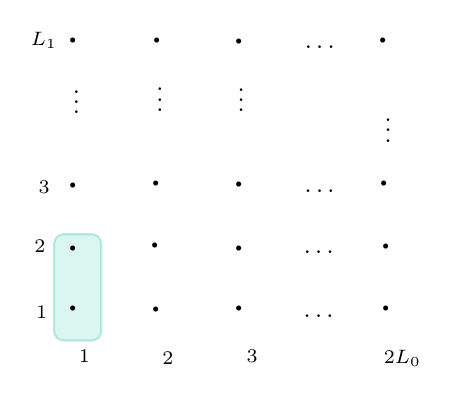
\begin{tikzpicture}[x=0.75pt,y=0.75pt,yscale=-1,xscale=1]
%uncomment if require: \path (0,300); %set diagram left start at 0, and has height of 300

%Rounded Rect [id:dp32613111558050933] 
\draw  [color={rgb, 255:red, 91; green, 210; blue, 185 }  ,draw opacity=0.41 ][fill={rgb, 255:red, 91; green, 210; blue, 185 }  ,fill opacity=0.22 ][line width=0.75]  (235.61,134.83) .. controls (235.61,132.33) and (237.64,130.3) .. (240.15,130.3) -- (253.75,130.3) .. controls (256.25,130.3) and (258.28,132.33) .. (258.28,134.83) -- (258.28,176.98) .. controls (258.28,179.48) and (256.25,181.51) .. (253.75,181.51) -- (240.15,181.51) .. controls (237.64,181.51) and (235.61,179.48) .. (235.61,176.98) -- cycle ;

% Text Node
\draw (240.42,31.05) node [anchor=north west][inner sep=0.75pt]  [font=\LARGE]  {$\cdot $};
% Text Node
\draw (243.37,52.51) node [anchor=north west][inner sep=0.75pt]  [font=\small]  {$\vdots $};
% Text Node
\draw (240.24,100.88) node [anchor=north west][inner sep=0.75pt]  [font=\LARGE]  {$\cdot $};
% Text Node
\draw (240.24,131.49) node [anchor=north west][inner sep=0.75pt]  [font=\LARGE]  {$\cdot $};
% Text Node
\draw (240.28,160.21) node [anchor=north west][inner sep=0.75pt]  [font=\LARGE]  {$\cdot $};
% Text Node
\draw (280.68,31.27) node [anchor=north west][inner sep=0.75pt]  [font=\LARGE]  {$\cdot $};
% Text Node
\draw (283.63,51.3) node [anchor=north west][inner sep=0.75pt]  [font=\small]  {$\vdots $};
% Text Node
\draw (280.36,100.29) node [anchor=north west][inner sep=0.75pt]  [font=\LARGE]  {$\cdot $};
% Text Node
\draw (279.76,130.1) node [anchor=north west][inner sep=0.75pt]  [font=\LARGE]  {$\cdot $};
% Text Node
\draw (280.11,160.87) node [anchor=north west][inner sep=0.75pt]  [font=\LARGE]  {$\cdot $};
% Text Node
\draw (320.17,31.67) node [anchor=north west][inner sep=0.75pt]  [font=\LARGE]  {$\cdot $};
% Text Node
\draw (322.72,51.5) node [anchor=north west][inner sep=0.75pt]  [font=\small]  {$\vdots $};
% Text Node
\draw (320.25,100.69) node [anchor=north west][inner sep=0.75pt]  [font=\LARGE]  {$\cdot $};
% Text Node
\draw (320.25,131.5) node [anchor=north west][inner sep=0.75pt]  [font=\LARGE]  {$\cdot $};
% Text Node
\draw (320.4,160.47) node [anchor=north west][inner sep=0.75pt]  [font=\LARGE]  {$\cdot $};
% Text Node
\draw (354.56,167.68) node [anchor=north west][inner sep=0.75pt]  [font=\small]  {$\dotsc $};
% Text Node
\draw (354.63,137.09) node [anchor=north west][inner sep=0.75pt]  [font=\small]  {$\dotsc $};
% Text Node
\draw (355.03,107.72) node [anchor=north west][inner sep=0.75pt]  [font=\small]  {$\dotsc $};
% Text Node
\draw (355.13,38.18) node [anchor=north west][inner sep=0.75pt]  [font=\small]  {$\dotsc $};
% Text Node
\draw (389.61,31.23) node [anchor=north west][inner sep=0.75pt]  [font=\LARGE]  {$\cdot $};
% Text Node
\draw (393.57,66.1) node [anchor=north west][inner sep=0.75pt]  [font=\small]  {$\vdots $};
% Text Node
\draw (390.23,100.27) node [anchor=north west][inner sep=0.75pt]  [font=\LARGE]  {$\cdot $};
% Text Node
\draw (391.23,130.48) node [anchor=north west][inner sep=0.75pt]  [font=\LARGE]  {$\cdot $};
% Text Node
\draw (390.85,160.43) node [anchor=north west][inner sep=0.75pt]  [font=\LARGE]  {$\cdot $};
% Text Node
\draw (246.25,184.84) node [anchor=north west][inner sep=0.75pt]  [font=\scriptsize]  {$1$};
% Text Node
\draw (286.45,185.75) node [anchor=north west][inner sep=0.75pt]  [font=\scriptsize]  {$2$};
% Text Node
\draw (327.04,184.77) node [anchor=north west][inner sep=0.75pt]  [font=\scriptsize]  {$3$};
% Text Node
\draw (393.19,184.87) node [anchor=north west][inner sep=0.75pt]  [font=\scriptsize]  {$2L_{0}$};
% Text Node
\draw (225.64,163.65) node [anchor=north west][inner sep=0.75pt]  [font=\scriptsize]  {$1$};
% Text Node
\draw (224.8,131.69) node [anchor=north west][inner sep=0.75pt]  [font=\scriptsize]  {$2$};
% Text Node
\draw (226.91,103.5) node [anchor=north west][inner sep=0.75pt]  [font=\scriptsize]  {$3$};
% Text Node
\draw (223.11,31.79) node [anchor=north west][inner sep=0.75pt]  [font=\scriptsize]  {$L_{1}$};


\end{tikzpicture}


    \caption{Visualization of the interaction along the space direction between two points of the first time slice.}
    \label{fig: space int}
\end{figure}
Consider for instance the interaction between the sites $1$ and $2$ on the first time slice (see Figure \eqref{fig: space int}), its expression is given by:
\begin{equation}
    - \left[ \begin{pmatrix}
        \Bar{\psi}^+_1 \,\, \Bar{\psi}^-_1
    \end{pmatrix} z_{1,2} (1 - \gamma_1) \begin{pmatrix}
        \psi^+_2 \\
        \psi^-_2
    \end{pmatrix} + \begin{pmatrix}
        \Bar{\psi}^+_2 \,\, \Bar{\psi}^-_2
    \end{pmatrix} \Bar{z}_{1,2} (1 + \gamma_1) \begin{pmatrix}
        \psi^+_1 \\
        \psi^-_1
    \end{pmatrix} \right]
\end{equation}
and using the explicit expression for $(1 \pm \gamma_1)$, it becomes:
\begin{equation}
    - z_{1,2} \left[ \Bar{\psi}^+_1 \psi_2^+ - \Bar{\psi}^+_1 \psi_2^- - \Bar{\psi}_1^-\psi_2^+ + \Bar{\psi}_1^- \psi_2^- \right] - \Bar{z}_{1,2} \left[ \Bar{\psi}^+_2 \psi_1^+ - \Bar{\psi}^+_2 \psi_1^- - \Bar{\psi}_2^-\psi_1^+ + \Bar{\psi}_2^- \psi_1^- \right]
\end{equation}
and for other pairs of sites we get analogous contributions. The mass term and the spatial interaction for the lattice sites lying on the first time slice can then be written compactly in a matrix form. Indeed, if we define:
\begin{equation}
    X_1 = \frac{1}{2} \begin{pmatrix}
        2 \Bar{m}_0 & - z_{1,2} & 0 & \dots & & 0 & - \Bar{z}_{L_1, 1} \\
        - \Bar{z}_{1,2} & 2 \Bar{m}_0 & - z_{2,3} & 0 & \dots & & 0 \\
        0 & - \Bar{z}_{2,3} & 2 \Bar{m}_0 & - z_{3,4} & 0 & \dots & \vdots \\
        \\
        \vdots & & & \ddots \\
        \\
        \\
        & & & & & & 0 \\
        0 & & & & - \Bar{z}_{L_1 - 2, L_1 - 1} & 2 \Bar{m}_0 & - z_{L_1 - 1, L_1} \\
        - z_{L_1, 1} & 0 & \dots & & 0 & - \Bar{z}_{L_1 - 1, L_1} & 2 \Bar{m}_0 \\ 
    \end{pmatrix}
\end{equation}
for which it holds $X_1 = X_1^{\dagger}$, i.e. it is hermitian, and:
\begin{equation}
    Y_1 = \frac{1}{2} \begin{pmatrix}
        0 & z_{1,2} & 0 & \dots & & 0 & - \Bar{z}_{L_1, 1} \\
        - \Bar{z}_{1,2} & 0 & z_{2,3} & 0 & \dots & & 0 \\
        0 & - \Bar{z}_{2,3} & 0 & - z_{3,4} & 0 & \dots & \vdots \\
        \\
        \vdots & & & \ddots \\
        \\
        \\
        & & & & & & 0 \\
        0 & & & & - \Bar{z}_{L_1 - 2, L_1 - 1} & 0 & - z_{L_1 - 1, L_1} \\
        - z_{L_1, 1} & 0 & \dots & & 0 & - \Bar{z}_{L_1 - 1, L_1} & 0 \\ 
    \end{pmatrix}
\end{equation}
which is an anti-hermitian matrix $Y_1 = - Y_1^\dagger$, then we can write the mass and spatial contribution to the Dirac operator for the first time slice as:
\begin{equation}
    D_1 = \begin{pmatrix}
        X_1 & Y_1 \\
        Y_1 & X_1 \\
    \end{pmatrix}
\end{equation}
and similarly for all the other time slices.
\begin{figure}
    \centering


\tikzset{every picture/.style={line width=0.75pt}} %set default line width to 0.75pt        

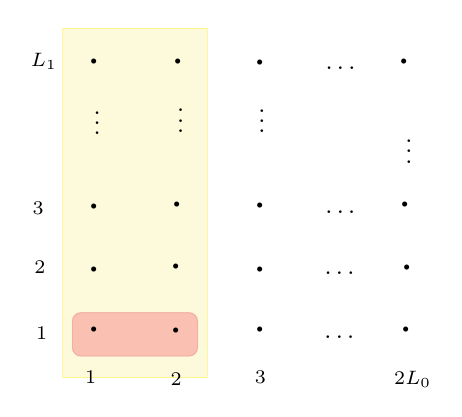
\begin{tikzpicture}[x=0.75pt,y=0.75pt,yscale=-1,xscale=1]
%uncomment if require: \path (0,300); %set diagram left start at 0, and has height of 300

%Shape: Rectangle [id:dp05909713682911022] 
\draw  [color={rgb, 255:red, 253; green, 239; blue, 52 }  ,draw opacity=0.49 ][fill={rgb, 255:red, 247; green, 235; blue, 109 }  ,fill opacity=0.24 ] (229.69,20.94) -- (299.36,20.94) -- (299.36,189.28) -- (229.69,189.28) -- cycle ;
%Rounded Rect [id:dp5474542337645614] 
\draw  [color={rgb, 255:red, 229; green, 124; blue, 125 }  ,draw opacity=0.41 ][fill={rgb, 255:red, 247; green, 134; blue, 134 }  ,fill opacity=0.49 ] (234.36,162.14) .. controls (234.36,159.82) and (236.24,157.94) .. (238.56,157.94) -- (290.49,157.94) .. controls (292.81,157.94) and (294.69,159.82) .. (294.69,162.14) -- (294.69,174.74) .. controls (294.69,177.06) and (292.81,178.94) .. (290.49,178.94) -- (238.56,178.94) .. controls (236.24,178.94) and (234.36,177.06) .. (234.36,174.74) -- cycle ;

% Text Node
\draw (240.42,31.05) node [anchor=north west][inner sep=0.75pt]  [font=\LARGE]  {$\cdot $};
% Text Node
\draw (243.37,52.51) node [anchor=north west][inner sep=0.75pt]  [font=\small]  {$\vdots $};
% Text Node
\draw (240.24,101.21) node [anchor=north west][inner sep=0.75pt]  [font=\LARGE]  {$\cdot $};
% Text Node
\draw (240.24,131.49) node [anchor=north west][inner sep=0.75pt]  [font=\LARGE]  {$\cdot $};
% Text Node
\draw (240.28,160.21) node [anchor=north west][inner sep=0.75pt]  [font=\LARGE]  {$\cdot $};
% Text Node
\draw (280.68,31.27) node [anchor=north west][inner sep=0.75pt]  [font=\LARGE]  {$\cdot $};
% Text Node
\draw (283.63,51.3) node [anchor=north west][inner sep=0.75pt]  [font=\small]  {$\vdots $};
% Text Node
\draw (280.36,100.29) node [anchor=north west][inner sep=0.75pt]  [font=\LARGE]  {$\cdot $};
% Text Node
\draw (279.76,130.1) node [anchor=north west][inner sep=0.75pt]  [font=\LARGE]  {$\cdot $};
% Text Node
\draw (280.11,160.87) node [anchor=north west][inner sep=0.75pt]  [font=\LARGE]  {$\cdot $};
% Text Node
\draw (320.17,31.67) node [anchor=north west][inner sep=0.75pt]  [font=\LARGE]  {$\cdot $};
% Text Node
\draw (322.72,51.5) node [anchor=north west][inner sep=0.75pt]  [font=\small]  {$\vdots $};
% Text Node
\draw (320.25,100.69) node [anchor=north west][inner sep=0.75pt]  [font=\LARGE]  {$\cdot $};
% Text Node
\draw (320.25,131.5) node [anchor=north west][inner sep=0.75pt]  [font=\LARGE]  {$\cdot $};
% Text Node
\draw (320.4,160.47) node [anchor=north west][inner sep=0.75pt]  [font=\LARGE]  {$\cdot $};
% Text Node
\draw (354.56,167.68) node [anchor=north west][inner sep=0.75pt]  [font=\small]  {$\dotsc $};
% Text Node
\draw (354.63,137.09) node [anchor=north west][inner sep=0.75pt]  [font=\small]  {$\dotsc $};
% Text Node
\draw (355.03,107.72) node [anchor=north west][inner sep=0.75pt]  [font=\small]  {$\dotsc $};
% Text Node
\draw (355.13,38.18) node [anchor=north west][inner sep=0.75pt]  [font=\small]  {$\dotsc $};
% Text Node
\draw (389.61,31.23) node [anchor=north west][inner sep=0.75pt]  [font=\LARGE]  {$\cdot $};
% Text Node
\draw (393.57,66.1) node [anchor=north west][inner sep=0.75pt]  [font=\small]  {$\vdots $};
% Text Node
\draw (390.23,100.27) node [anchor=north west][inner sep=0.75pt]  [font=\LARGE]  {$\cdot $};
% Text Node
\draw (391.23,130.48) node [anchor=north west][inner sep=0.75pt]  [font=\LARGE]  {$\cdot $};
% Text Node
\draw (390.85,160.43) node [anchor=north west][inner sep=0.75pt]  [font=\LARGE]  {$\cdot $};
% Text Node
\draw (239.25,184.84) node [anchor=north west][inner sep=0.75pt]  [font=\scriptsize]  {$1$};
% Text Node
\draw (280.45,185.75) node [anchor=north west][inner sep=0.75pt]  [font=\scriptsize]  {$2$};
% Text Node
\draw (321.04,184.77) node [anchor=north west][inner sep=0.75pt]  [font=\scriptsize]  {$3$};
% Text Node
\draw (388.19,184.87) node [anchor=north west][inner sep=0.75pt]  [font=\scriptsize]  {$2L_{0}$};
% Text Node
\draw (215.64,163.65) node [anchor=north west][inner sep=0.75pt]  [font=\scriptsize]  {$1$};
% Text Node
\draw (214.8,131.69) node [anchor=north west][inner sep=0.75pt]  [font=\scriptsize]  {$2$};
% Text Node
\draw (213.91,103.5) node [anchor=north west][inner sep=0.75pt]  [font=\scriptsize]  {$3$};
% Text Node
\draw (213.11,31.79) node [anchor=north west][inner sep=0.75pt]  [font=\scriptsize]  {$L_{1}$};


\end{tikzpicture}

    \caption{Visualization of the interaction along the time direction between $1$ and $L_1 + 1$, the first sites of the time slices 1 and 2, i.e. Eq. \eqref{time inter}.}
    \label{fig: time int}
\end{figure}
\\ The last contribution we should consider comes from interactions in the time direction, for instance:
\begin{equation}
    - \left[ \Bar{\psi}(n) \left(1 - \gamma_0 \right) U_0(x) \psi(n + \hat{0}) + \Bar{\psi}(n + \hat{0}) \left(1 + \gamma_0 \right) U^\dagger_0(x) \psi(n) \right]
\end{equation}
and analogously to what we have done for spatial contributions, we can write the interaction between two points $1$ and $L_1 + 1$ explicitly as (see Fig. \eqref{fig: time int}):
\begin{equation}\label{time inter}
    \begin{split}
        &- 2 \left[ \begin{pmatrix}
        \Bar{\psi}^+_1 \,\, \Bar{\psi}^-_1
    \end{pmatrix} z_{1,L_1 + 1} (1 - \gamma_0) \begin{pmatrix}
        \psi^+_{L_1 + 1} \\
        \psi^-_{L_1 + 1}
    \end{pmatrix} + \begin{pmatrix}
        \Bar{\psi}^+_{L_1 + 1} \,\, \Bar{\psi}^-_{L_1 + 1}
    \end{pmatrix} \Bar{z}_{1,L_1 + 1} (1 + \gamma_0) \begin{pmatrix}
        \psi^+_1 \\
        \psi^-_1
    \end{pmatrix} \right] = \\
   & = -2 \left[ z_{1, L_1 + 1} \Bar{\psi}_1^+ \psi_{L_1 + 1}^+ + \Bar{z}_{1, L_1 + 1} \Bar{\psi}_{L_1 + 1}^- \psi_1^- \right]
    \end{split}
\end{equation}
Notice that these contributions are diagonal in the chiral components. We can thus define the matrix:
\begin{equation}
    \Lambda_{1, L_1 + 1} = - \begin{pmatrix}
        z_{1, L_1 + 1} & 0 & \dots &  & & 0  \\
        0 & z_{2, L_1 + 2} & 0 & \dots &  & \vdots \\
        \vdots & 0 & \ddots & 0 \\
        \\
        & & & & &  0 \\
        0 & & & \dots & 0 & z_{L_1, 2L_1} \\ 
    \end{pmatrix} = \Lambda^{T}_{1, L_1 + 1}
\end{equation}
and consequently the contributions to the Dirac operator coming from interactions along the time direction between the first two time slices can be expressed with the following matrices:
\begin{equation} \label{time interaction matrix}
    D_{1, L_1 + 1} = \begin{pmatrix}
        \Lambda_{1, L_1 + 1} & \mathbb{0} \\
        \mathbb{0} & \mathbb{0} \\
    \end{pmatrix} \hspace{10mm} \Tilde{D}_{1, L_1 + 1} = \begin{pmatrix}
        \mathbb{0} & \mathbb{0} \\
        \mathbb{0} & \Bar{\Lambda}_{1, L_1 + 1} \\
    \end{pmatrix}
\end{equation}
and analogously for the other time slices\footnote{Notice that in the following sections $\mathbb{0}$ typically represents a $L_1 \cross L_1$ block of zeros, unless otherwise stated, but in any case its dimensions should be clear from the context. For instance, in definition \eqref{D matrix} it has dimensions $2L_1 \cross 2L_1.$}. 
\\ Taking into account all the contributions, we can write the Dirac operator as:
\begin{equation}\label{D matrix}
    \mathcal{D} = \begin{pmatrix}
        D_1 & D_{1,2} & \mathbb{0} & \dots &  & \Tilde{J}  \\
        \Tilde{D}_{1,2} & D_2 & D_{2,3} & \mathbb{0} & \dots & \mathbb{0} \\
        \mathbb{0} & \Tilde{D}_{2,3} & D_3 & D_{3,4} & \mathbb{0} & \vdots \\
        \vdots & & & \ddots & \\
        \\
        \mathbb{0} & & & & D_{2L_0 - 1} & D_{2L_0 - 1, 2L_0} \\
        J & \mathbb{0} & \dots & \mathbb{0} & \Tilde{D}_{2L_0 - 1, 2L_0} & D_{2L_0} \\ 
    \end{pmatrix}
\end{equation}
where:
\begin{equation}
    J = \left\{ \begin{array}{rcl} \mathbb{0} \hspace{10mm} \mbox{open boundary conditions}& \\ D_{L_0, 1}  \hspace{3mm} \mbox{periodic boundary conditions}&  \\ \end{array} \right.
\end{equation}
The expression \eqref{D matrix} for the Dirac operator allows us to write the fermion action in a quadratic form, hence when we integrate out the Grassmann variables in the path integral we get:
\begin{equation}
    \int \mathcal{D}[\psi] \mathcal{D}[\Bar{\psi}] e^{-\Bar{\psi} \mathcal{D} \psi} = \det(\mathcal{D})
\end{equation}

\section{Open boundary conditions}\label{OpenBC}
\begin{figure}
    \centering
\tikzset{every picture/.style={line width=0.75pt}} %set default line width to 0.75pt        
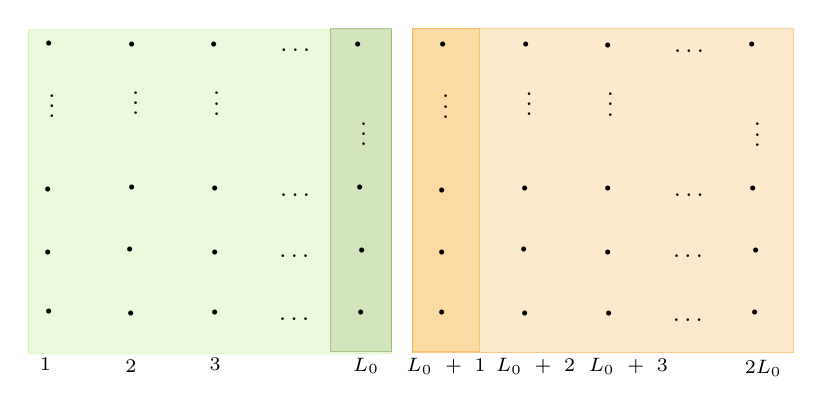
\begin{tikzpicture}[x=0.75pt,y=0.75pt,yscale=-1,xscale=1]
%uncomment if require: \path (0,300); %set diagram left start at 0, and has height of 300

%Shape: Rectangle [id:dp3848625804971728] 
\draw  [color={rgb, 255:red, 184; green, 233; blue, 134 }  ,draw opacity=0.46 ][fill={rgb, 255:red, 184; green, 233; blue, 134 }  ,fill opacity=0.28 ] (234.89,30) -- (410.03,30) -- (410.03,185.94) -- (234.89,185.94) -- cycle ;
%Shape: Rectangle [id:dp9450776254434018] 
\draw  [color={rgb, 255:red, 65; green, 117; blue, 5 }  ,draw opacity=0.29 ][fill={rgb, 255:red, 65; green, 117; blue, 5 }  ,fill opacity=0.15 ] (380.36,29.33) -- (410.03,29.33) -- (410.03,185.28) -- (380.36,185.28) -- cycle ;
%Shape: Rectangle [id:dp43101617233074474] 
\draw  [color={rgb, 255:red, 245; green, 166; blue, 35 }  ,draw opacity=0.47 ][fill={rgb, 255:red, 245; green, 166; blue, 35 }  ,fill opacity=0.23 ] (419.89,29.67) -- (603.69,29.67) -- (603.69,185.61) -- (419.89,185.61) -- cycle ;
%Shape: Rectangle [id:dp31365082950207435] 
\draw  [color={rgb, 255:red, 245; green, 166; blue, 35 }  ,draw opacity=0.46 ][fill={rgb, 255:red, 245; green, 166; blue, 35 }  ,fill opacity=0.24 ] (419.89,29.67) -- (452.36,29.67) -- (452.36,185.28) -- (419.89,185.28) -- cycle ;

% Text Node
\draw (240.42,31.05) node [anchor=north west][inner sep=0.75pt]  [font=\LARGE]  {$\cdot $};
% Text Node
\draw (243.37,52.51) node [anchor=north west][inner sep=0.75pt]  [font=\small]  {$\vdots $};
% Text Node
\draw (240.24,101.21) node [anchor=north west][inner sep=0.75pt]  [font=\LARGE]  {$\cdot $};
% Text Node
\draw (240.24,131.49) node [anchor=north west][inner sep=0.75pt]  [font=\LARGE]  {$\cdot $};
% Text Node
\draw (240.28,160.21) node [anchor=north west][inner sep=0.75pt]  [font=\LARGE]  {$\cdot $};
% Text Node
\draw (280.68,31.27) node [anchor=north west][inner sep=0.75pt]  [font=\LARGE]  {$\cdot $};
% Text Node
\draw (283.63,51.3) node [anchor=north west][inner sep=0.75pt]  [font=\small]  {$\vdots $};
% Text Node
\draw (280.36,100.29) node [anchor=north west][inner sep=0.75pt]  [font=\LARGE]  {$\cdot $};
% Text Node
\draw (279.76,130.1) node [anchor=north west][inner sep=0.75pt]  [font=\LARGE]  {$\cdot $};
% Text Node
\draw (280.11,160.87) node [anchor=north west][inner sep=0.75pt]  [font=\LARGE]  {$\cdot $};
% Text Node
\draw (320.17,31.67) node [anchor=north west][inner sep=0.75pt]  [font=\LARGE]  {$\cdot $};
% Text Node
\draw (322.72,51.5) node [anchor=north west][inner sep=0.75pt]  [font=\small]  {$\vdots $};
% Text Node
\draw (320.25,100.69) node [anchor=north west][inner sep=0.75pt]  [font=\LARGE]  {$\cdot $};
% Text Node
\draw (320.25,131.5) node [anchor=north west][inner sep=0.75pt]  [font=\LARGE]  {$\cdot $};
% Text Node
\draw (320.4,160.47) node [anchor=north west][inner sep=0.75pt]  [font=\LARGE]  {$\cdot $};
% Text Node
\draw (354.56,167.68) node [anchor=north west][inner sep=0.75pt]  [font=\small]  {$\dotsc $};
% Text Node
\draw (354.63,137.09) node [anchor=north west][inner sep=0.75pt]  [font=\small]  {$\dotsc $};
% Text Node
\draw (355.03,107.72) node [anchor=north west][inner sep=0.75pt]  [font=\small]  {$\dotsc $};
% Text Node
\draw (355.13,38.18) node [anchor=north west][inner sep=0.75pt]  [font=\small]  {$\dotsc $};
% Text Node
\draw (389.61,31.23) node [anchor=north west][inner sep=0.75pt]  [font=\LARGE]  {$\cdot $};
% Text Node
\draw (393.57,66.1) node [anchor=north west][inner sep=0.75pt]  [font=\small]  {$\vdots $};
% Text Node
\draw (390.23,100.27) node [anchor=north west][inner sep=0.75pt]  [font=\LARGE]  {$\cdot $};
% Text Node
\draw (391.23,130.48) node [anchor=north west][inner sep=0.75pt]  [font=\LARGE]  {$\cdot $};
% Text Node
\draw (390.85,160.43) node [anchor=north west][inner sep=0.75pt]  [font=\LARGE]  {$\cdot $};
% Text Node
\draw (239.25,186.84) node [anchor=north west][inner sep=0.75pt]  [font=\scriptsize]  {$1$};
% Text Node
\draw (280.45,187.75) node [anchor=north west][inner sep=0.75pt]  [font=\scriptsize]  {$2$};
% Text Node
\draw (321.04,186.77) node [anchor=north west][inner sep=0.75pt]  [font=\scriptsize]  {$3$};
% Text Node
\draw (390.19,186.87) node [anchor=north west][inner sep=0.75pt]  [font=\scriptsize]  {$L_{0}$};
% Text Node
\draw (430.09,31.4) node [anchor=north west][inner sep=0.75pt]  [font=\LARGE]  {$\cdot $};
% Text Node
\draw (433.03,52.87) node [anchor=north west][inner sep=0.75pt]  [font=\small]  {$\vdots $};
% Text Node
\draw (429.91,101.57) node [anchor=north west][inner sep=0.75pt]  [font=\LARGE]  {$\cdot $};
% Text Node
\draw (429.91,131.85) node [anchor=north west][inner sep=0.75pt]  [font=\LARGE]  {$\cdot $};
% Text Node
\draw (429.95,160.56) node [anchor=north west][inner sep=0.75pt]  [font=\LARGE]  {$\cdot $};
% Text Node
\draw (470.35,31.62) node [anchor=north west][inner sep=0.75pt]  [font=\LARGE]  {$\cdot $};
% Text Node
\draw (473.3,51.65) node [anchor=north west][inner sep=0.75pt]  [font=\small]  {$\vdots $};
% Text Node
\draw (470.03,100.65) node [anchor=north west][inner sep=0.75pt]  [font=\LARGE]  {$\cdot $};
% Text Node
\draw (469.43,130.45) node [anchor=north west][inner sep=0.75pt]  [font=\LARGE]  {$\cdot $};
% Text Node
\draw (469.78,161.22) node [anchor=north west][inner sep=0.75pt]  [font=\LARGE]  {$\cdot $};
% Text Node
\draw (509.83,32.02) node [anchor=north west][inner sep=0.75pt]  [font=\LARGE]  {$\cdot $};
% Text Node
\draw (512.38,51.85) node [anchor=north west][inner sep=0.75pt]  [font=\small]  {$\vdots $};
% Text Node
\draw (509.91,101.05) node [anchor=north west][inner sep=0.75pt]  [font=\LARGE]  {$\cdot $};
% Text Node
\draw (509.91,131.85) node [anchor=north west][inner sep=0.75pt]  [font=\LARGE]  {$\cdot $};
% Text Node
\draw (510.07,160.82) node [anchor=north west][inner sep=0.75pt]  [font=\LARGE]  {$\cdot $};
% Text Node
\draw (544.23,168.03) node [anchor=north west][inner sep=0.75pt]  [font=\small]  {$\dotsc $};
% Text Node
\draw (544.3,137.45) node [anchor=north west][inner sep=0.75pt]  [font=\small]  {$\dotsc $};
% Text Node
\draw (544.7,108.08) node [anchor=north west][inner sep=0.75pt]  [font=\small]  {$\dotsc $};
% Text Node
\draw (544.79,38.53) node [anchor=north west][inner sep=0.75pt]  [font=\small]  {$\dotsc $};
% Text Node
\draw (579.28,31.58) node [anchor=north west][inner sep=0.75pt]  [font=\LARGE]  {$\cdot $};
% Text Node
\draw (583.24,66.45) node [anchor=north west][inner sep=0.75pt]  [font=\small]  {$\vdots $};
% Text Node
\draw (579.9,100.62) node [anchor=north west][inner sep=0.75pt]  [font=\LARGE]  {$\cdot $};
% Text Node
\draw (580.9,130.83) node [anchor=north west][inner sep=0.75pt]  [font=\LARGE]  {$\cdot $};
% Text Node
\draw (580.52,160.78) node [anchor=north west][inner sep=0.75pt]  [font=\LARGE]  {$\cdot $};
% Text Node
\draw (415.92,187.2) node [anchor=north west][inner sep=0.75pt]  [font=\scriptsize]  {$L_{0} \ +\ 1$};
% Text Node
\draw (459.11,187.1) node [anchor=north west][inner sep=0.75pt]  [font=\scriptsize]  {$L_{0} \ +\ 2$};
% Text Node
\draw (503.71,187.13) node [anchor=north west][inner sep=0.75pt]  [font=\scriptsize]  {$L_{0} \ +\ 3$};
% Text Node
\draw (578.86,188.22) node [anchor=north west][inner sep=0.75pt]  [font=\scriptsize]  {$2L_{0}$};


\end{tikzpicture}

    \caption{Lattice decomposition in the case of open boundary conditions. We split the system in two regions, where we identify a core part (lighter color) and a shell part (darker color).}
    \label{fig: fig op bc}
\end{figure}
Consider the system described in the previous section. If we employ open boundary conditions, the blocks labelled as $J$ and $\Tilde{J}$ in \eqref{D matrix} vanish, and $\mathcal{D}$ becomes a sparse tri-diagonal block matrix. To proceed towards the factorization of $\det (\mathcal{D})$, we need to split the system dynamics into two halves, described respectively by the first $L_0$ time slices $[1, L_0]$ and the latter ones $[L_0 + 1, 2L_0]$.
\\ For both subsystems we can recognize a \textit{core} part, given respectively by the time slices $[1, L_0 - 1]$ and $[L_0 + 2, 2L_0]$, and a \textit{shell} part, given by the time slice $L_0$ and $L_0 + 1$. See Figure \eqref{fig: fig op bc}.
\\ In order to better visualize the following steps, it is convenient to rewrite $\mathcal{D}$ making these separations explicit:
\begin{equation}
    \mathcal{D} = \begin{pmatrix}
         \mathcal{D}_{1, L_0 - 1} & & A & & \mathbb{0}_{L_0 +- 1} \\
         \\
          & D_{L_0} & & D_{L_0, L_0 + 1} &  \\
          B & & & & E \\
          &  \Tilde{D}_{L_0, L_0 + 1} & &  D_{L_0 + 1} & \\
          \\
         \mathbb{0}_{L_0 - 1} & & F & & \mathcal{D}_{L_0 + 2, 2L_0}
    \end{pmatrix}
\end{equation}
where $\mathcal{D}_{1, L_0 - 1}$ and $\mathcal{D}_{L_0 - 1, 2L_0}$ denote the blocks of the Dirac operator associated with the core time slices, $\mathbb{0}_{L_0 - 1}$ is a matrix of zeros with the same dimensions as $\mathcal{D}_{1, L_0 - 1}$ and $\mathcal{D}_{L_0 - 1, 2L_0}$, while:
\begin{equation*}
    A = \begin{pmatrix}
         \mathbb{0} & \mathbb{0} \\
        \vdots & \vdots \\
        \mathbb{0} & \mathbb{0} \\
        D_{L_0 - 1, L_0} & \mathbb{0} \\
    \end{pmatrix} \hspace{5mm} B = \begin{pmatrix}
        \mathbb{0} & \dots & \mathbb{0} & \Tilde{D}_{L_0-1, L_0} \\
        \mathbb{0} & \dots & \mathbb{0} & \mathbb{0} \\
    \end{pmatrix}
\end{equation*}
\begin{equation}
    E = \begin{pmatrix}
        \mathbb{0} & \mathbb{0} & \dots & \mathbb{0} \\
        D_{L_0 + 1, L_0 + 2} & \mathbb{0} & \dots & \mathbb{0} \\
    \end{pmatrix} \hspace{5mm} F = \begin{pmatrix}
        \mathbb{0} & \dots & \mathbb{0} & \Tilde{D}_{L_0+1, L_0+2} \\
        \mathbb{0} & \dots & \mathbb{0} & \mathbb{0}\\
    \end{pmatrix}
\end{equation}
We can use the Schur decomposition reported in \eqref{Schur} to write:
\begin{equation}\label{D decomp M N}
    \det(\mathcal{D}) = \det(\mathcal{D}_{1, L_0 - 1}) \det (\mathcal{D}_{L_0 + 1, 2L_0}) \det \begin{pmatrix}
        M_{L_0} & D_{L_0, L_0 + 1} \\
        \Tilde{D}_{L_0, L_0 + 1} & N_{L_0 + 1}
    \end{pmatrix} 
\end{equation}
where $M_{L_0}$ and $N_{L_0 + 1}$ are the Schur complements defined as:
\begin{equation}\label{M and N}
    \begin{split}
        M_{L_0} = D_{L_0} - \Tilde{D}_{L_0 - 1, L_0} R_A^{-1} D_{L_0 - 1, L_0} \\
        N_{L_0 + 1} = D_{L_0 + 1} - D_{L_0 + 1, L_0 + 2} R_B^{-1} \Tilde{D}_{L_0 + 1, L_0 +2}
    \end{split}
\end{equation}
with $R_A^{-1}$ and $R_B^{-1}$ being respectively the block matrix in the lower-right corner of $\mathcal{D}_{1, L_0 - 1}^{-1}$ and the block matrix in the upper-left corner of $\mathcal{D}_{L_0 + 1, 2L_0}^{-1}$:
\begin{equation}
    \mathcal{D}_{1, L_0 - 1}^{-1} = \begin{pmatrix}
        & \dots & &  \\
        \vdots & \ddots \\
        & & \\
         &  &  & R_A^{-1} \\
    \end{pmatrix} \hspace{5mm}  \mathcal{D}_{L_0 + 1, 2L_0}^{-1} = \begin{pmatrix}
        R_B^{-1} &  \\
         & & &  \\
        & & \ddots & \vdots \\
         & & \dots & \\
    \end{pmatrix}
\end{equation}
Given the structure of the Dirac operator, $R_A^{-1}$ and $R_B^{-1}$ will be of the form:
\begin{equation}
    R_A^{-1} = \begin{pmatrix}
        Z_A & W_A \\
        W_A & Z_A \\
    \end{pmatrix} \hspace{5 mm}  R_B^{-1} = \begin{pmatrix}
        Z_B & W_B \\
        W_B & Z_B \\
    \end{pmatrix}
\end{equation}
Notice that it is not necessary to compute the whole core blocks $\mathcal{D}_{1, L_0 - 1}^{-1}$ and $\mathcal{D}_{L_0 + 1, 2L_0}^{-1}$ to find $R_A^{-1}$ and $R_B^{-1}$, since we can make use of the relation \eqref{matrix inverse} and the fact that the core blocks matrices are sparse.
\\ It is useful to recast the expressions of Eq. \eqref{M and N} more explicitly. Given the previous definitions \eqref{time interaction matrix}, it is easy to see that:
\begin{equation}
    \Tilde{D}_{L_0 - 1, L_0} R_A^{-1} D_{L_0 - 1, L_0} = \begin{pmatrix}
        \mathbb{0} & \mathbb{0} \\
        \Bar{\Lambda}_{L_0 - 1, L_0} W_A \Lambda_{L_0 - 1, L_0} & \mathbb{0} \\
    \end{pmatrix}
\end{equation}
and
\begin{equation}
    D_{L_0 + 1, L_0 + 2} R_B^{-1} \Tilde{D}_{L_0 + 1, L_0 + 2} = \begin{pmatrix}
        \mathbb{0} & \Lambda_{L_0 + 1, L_0 + 2} W_B \Bar{\Lambda}_{L_0 + 1, L_0 + 2} \\
        \mathbb{0} & \mathbb{0} \\
    \end{pmatrix}
\end{equation}
Consequently, the Schur complements become:
\begin{equation}
    M_{L_0} = D_{L_0} -  \Tilde{D}_{L_0 - 1, L_0} R_A^{-1} D_{L_0 - 1, L_0} = \begin{pmatrix}
        X_{L_0} & Y_{L_0} \\
       \Tilde{Y}_{L_0} & X_{L_0} \\ 
    \end{pmatrix}
\end{equation}
\begin{equation}
    N_{L_0 + 1} = D_{L_0 + 1} -  D_{L_0 + 1, L_0 + 2} R_B^{-1} \Tilde{D}_{L_0 + 1, L_0 + 2} = \begin{pmatrix}
        X_{L_0 + 1} & \Tilde{Y}_{L_0 + 1} \\
        Y_{L_0 + 1} & X_{L_0 + 1} \\ 
    \end{pmatrix}
\end{equation}
with $\Tilde{Y}_{L_0} = Y_{L_0} - \Bar{\Lambda}_{L_0 - 1, L_0} W_A \Lambda_{L_0 - 1, L_0}$ and $\Tilde{Y}_{L_0 + 1} = Y_{L_0 + 1} - \Lambda_{L_0 + 1, L_0 + 2} W_B \Bar{\Lambda}_{L_0 - 1, L_0}$.
\\ Then we can rewrite the third matrix on the RHS of \eqref{D decomp M N} as:
\begin{equation}
    d = \begin{pmatrix}
        X_{L_0} & Y_{L_0} & \Lambda_{L_0, L_0 + 1} & \mathbb{0} \\
        \Tilde{Y}_{L_0} & X_{L_0} & \mathbb{0} & \mathbb{0} \\
        \mathbb{0} & \mathbb{0} & X_{L_0 + 1} & \Tilde{Y}_{L_0 + 1} \\
        \mathbb{0} & \Bar{\Lambda}_{L_0, L_0 + 1} & Y_{L_0 + 1} & X_{L_0 + 1} \\ 
    \end{pmatrix}
\end{equation}
Since we are interested in $\det (d)$, we can perform a rotation that leaves the determinant invariant:
\begin{equation}\label{rot}
    \begin{pmatrix}
        \mathbb{0} & \mathbb{0} & \mathbb{1} & \mathbb{0} \\
        \mathbb{0} & \mathbb{1} & \mathbb{0} & \mathbb{0} \\
        \mathbb{1} & \mathbb{0} & \mathbb{0} & \mathbb{0} \\
        \mathbb{0} & \mathbb{0} & \mathbb{0} & \mathbb{1} \\
    \end{pmatrix} d \begin{pmatrix}
        \mathbb{1} & \mathbb{0} & \mathbb{0} & \mathbb{0} \\
        \mathbb{0} & \mathbb{0} & \mathbb{0} & \mathbb{1} \\
        \mathbb{0} & \mathbb{0} & \mathbb{1} & \mathbb{0} \\
        \mathbb{0} & \mathbb{1} & \mathbb{0} & \mathbb{0} \\
    \end{pmatrix} = \begin{pmatrix}
        \mathbb{0} & \Tilde{Y}_{L_0 + 1} & X_{L_0 + 1} & \mathbb{0} \\
        \Tilde{Y}_{L_0} & \mathbb{0} & \mathbb{0} & X_{L_0} \\
        X_{L_0} & \mathbb{0} & \Lambda_{L_0, L_0 + 1} & Y_{L_0} \\
        \mathbb{0} & X_{L_0 + 1} & Y_{L_0 + 1} & \Bar{\Lambda}_{L_0, L_0 + 1} \\
    \end{pmatrix}
\end{equation}
Then, if we assume that $\Tilde{Y}$ dimension is even, we can make use of the Schur decomposition \eqref{Schur} again to express the determinant of $d$ as:
\begin{equation}\label{det d}
    \det(d) = \det(\Tilde{Y}_{L_0}) \det(\Tilde{Y}_{L_0 + 1}) \det(\Tilde{d})
\end{equation}
where $\Tilde{d}$ is the defined as the Schur complement with respect to the lower right block of the matrix on the RHS of \eqref{rot}:
\begin{equation}
    \Tilde{d} = \begin{pmatrix}
        \Lambda_{L_0, L_0 + 1} & Y_{L_0} \\
        Y_{L_0 + 1} & \Bar{\Lambda}_{L_0, L_0 + 1} \\ 
    \end{pmatrix} - \begin{pmatrix}
        X_{L_0} & \mathbb{0} \\
        \mathbb{0} &  X_{L_0 + 1} \\ 
    \end{pmatrix} \begin{pmatrix}
        \mathbb{0} & \Tilde{Y}_{L_0}^{-1} \\
        \Tilde{Y}_{L_0 + 1}^{-1} & \mathbb{0} \\ 
    \end{pmatrix}\begin{pmatrix}
        X_{L_0 + 1} & \mathbb{0} \\
        \mathbb{0} &  X_{L_0} \\ 
    \end{pmatrix}
\end{equation}
\begin{equation}
    \rightarrow \Tilde{d} = \begin{pmatrix}
        \Lambda_{L_0, L_0 + 1} & Y_{L_0} - X_{L_0} (\Tilde{Y}_{L_0})^{-1} X_{L_0} \\
        Y_{L_0 + 1} - X_{L_0 + 1} (\Tilde{Y}_{L_0 + 1})^{-1} X_{L_0 + 1} & \Bar{\Lambda}_{L_0, L_0 + 1} \\ 
    \end{pmatrix}
\end{equation}
If we now introduce the following unitary matrices:
\begin{equation}
    \lambda_{L_0, L_0 + 1} = \sqrt{\Lambda_{L_0, L_0 + 1}} \hspace{4mm} \Bar{\lambda}_{L_0, L_0 + 1} = \sqrt{\Bar{\Lambda}_{L_0, L_0 + 1}} \longrightarrow \lambda_i \Bar{\lambda}_i = \mathbb{1}
\end{equation}
we can perform another convenient multiplication which leaves $\det(\Tilde{d})$ invariant:
\begin{equation}
    \begin{pmatrix}
        \Bar{\lambda}_{L_0, L_0 + 1} & \mathbb{0} \\
        \mathbb{0} & \lambda_{L_0, L_0 + 1} \\
    \end{pmatrix} \Tilde{d} \begin{pmatrix}
        \Bar{\lambda}_{L_0, L_0 + 1} & \mathbb{0} \\
        \mathbb{0} & \lambda_{L_0, L_0 + 1} \\
    \end{pmatrix} = \begin{pmatrix}
        \mathbb{1} & \hat{Y}_{L_0} \\
        \hat{Y}_{L_0 + 1} & \mathbb{1} \\
    \end{pmatrix} 
\end{equation}
where:
\begin{equation}\label{Y hat}
\begin{split}
        \hat{Y}_{L_0} &= \Bar{\lambda}_{L_0, L_0 + 1} \left[ Y_{L_0} - X_{L_0} (\Tilde{Y}_{L_0})^{-1} X_{L_0} \right] \lambda_{L_0, L_0 + 1} \\
    \hat{Y}_{L_0 + 1} &= \lambda_{L_0, L_0 + 1} \left[ Y_{L_0 + 1} - X_{L_0 + 1} (\Tilde{Y}_{L_0 + 1})^{-1} X_{L_0 + 1} \right] \Bar{\lambda}_{L_0, L_0 + 1} \\
\end{split}
\end{equation}
Putting \eqref{D decomp M N} and \eqref{det d} together, we have that:
\begin{equation}\label{last step fact}
    \det(\mathcal{D}) = \det(\mathcal{D}_{1, L_0 - 1}) \det(\mathcal{D}_{L_0 + 1, 2L_0}) \det(\Tilde{Y}_{L_0})  \det(\Tilde{Y}_{L_0 + 1}) \det(\Tilde{d})
\end{equation}
hence the contributions coming from the different domains $[1, L_0]$ and $[L_0 + 1, 2L_0]$ are factorized in all the previous determinants, with the exception of $\det(\Tilde{d})$.
\\ In order to achieve a complete factorization, it is useful to express the determinant of $\Tilde{d}$ in terms of its Pfaffian:
\begin{equation}
    \det(\Tilde{d}) = \left[ \textrm{Pf}(\Tilde{d}) \right]^2 = \textrm{Pf} \begin{pmatrix}
        \mathbb{0} & \Tilde{d} \\
        - \Tilde{d}^{T} & \mathbb{0} \\
    \end{pmatrix} = \textrm{Pf}(M)
\end{equation}
where $M$ is given by:
\begin{equation}
    M = \begin{pmatrix}
        \mathbb{0} & \mathbb{0} & \mathbb{1} & \hat{Y}_{L_0} \\
        \mathbb{0} & \mathbb{0} & \hat{Y}_{L_0 + 1} & \mathbb{1} \\
        -\mathbb{1} & - \hat{Y}_{L_0 + 1}^{T} & \mathbb{0} & \mathbb{0} \\
        - \hat{Y}_{L_0}^{T} & - \mathbb{1} & \mathbb{0} & \mathbb{0} \\
        
    \end{pmatrix}
\end{equation}
Since all the blocks of $M$ are of even dimensions, we can exchange the order of rows and columns without taking additive signs. Indeed, if we swap rows and columns $2 \leftrightarrow 4$, the matrix becomes:
\begin{equation}
    M = \begin{pmatrix}
        \mathbb{0} & \hat{Y}_{L_0} & \mathbb{1} & \mathbb{0} \\
        - \hat{Y}_{L_0 + 1}^{T} & \mathbb{0} & \mathbb{0} & -\mathbb{1} \\
         -\mathbb{1} & \mathbb{0} & \mathbb{0} & - \hat{Y}_{L_0 + 1}^{T} \\
         \mathbb{0} & \mathbb{1} & \hat{Y}_{L_0 + 1} & \mathbb{0} \\
    \end{pmatrix}
\end{equation}
We can now perform a rotation represented by the matrix:
\begin{equation}
    R = \begin{pmatrix}
        U & 0 \\
        0 & U \\
    \end{pmatrix} \begin{pmatrix}
        V & 0 \\
        0 & V \\
    \end{pmatrix} \begin{pmatrix}
        i\mathbb{1} & 0 \\
        0 & \mathbb{1} \\
    \end{pmatrix} \begin{pmatrix}
        Z & 0 \\
        0 & \mathbb{1}
    \end{pmatrix} = \begin{pmatrix}
        R_+ & 0 \\
        0 & R_- \\
    \end{pmatrix}
\end{equation}
with the definitions:
\begin{equation}
\begin{split}
    U = \frac{1}{\sqrt{2}} \begin{pmatrix}
        1 & -1 \\
        1 & 1 \\
    \end{pmatrix} \hspace{3mm} V = \begin{pmatrix}
        0 & i \\
        1 & 0 \\
    \end{pmatrix} \hspace{3mm} Z = \begin{pmatrix}
        0 & 1 \\
        1 & 0 \\
    \end{pmatrix} \\ \mbox{and} \hspace{2mm} R_+ = - \frac{1}{\sqrt{2}} \begin{pmatrix}
        1 & i \\
        1 & -i \\
    \end{pmatrix} \hspace{3mm} R_- = \frac{1}{\sqrt{2}}\begin{pmatrix}
        -1 & i \\
        1 & i \\
    \end{pmatrix}
\end{split}
\end{equation}
Since all the block matrices are of even dimensions, the Pfaffian of $M$ is left invariant by the rotation $M' = R^T M R$:
\begin{equation}
    \textrm{Pf}(M) = \textrm{Pf}(R^{T} M R) = \det(R) \textrm{Pf}(M)
\end{equation}
Let's give a closer look to $M'$. If we divide $M$ in four blocks, we have that:
\begin{equation}
    \begin{pmatrix}
        R_+^T & \mathbb{0} \\
        \\
        \mathbb{0} & R_-^T \\
    \end{pmatrix}\begin{pmatrix}
        M_{1,1} & M_{1,2} \\
        \\
        -M_{1,2} & M_{2,2} \\
    \end{pmatrix}\begin{pmatrix}
        R_+ & \mathbb{0} \\
        \\
        \mathbb{0} & R_- \\
    \end{pmatrix} = \begin{pmatrix}
        R_+^T M_{1,1} R_+ & R_+^T M_{1,2} R_- \\
        \\
        -R_-^T M_{2,1} R_+ & R_-^T M_{2,2}R_- \\
    \end{pmatrix}
\end{equation}
and from the previous definitions:
\begin{equation}
   K_{L_0} = R_+^T M_{1,1} R_+ = \frac{1}{2}\begin{pmatrix}
        \hat{Y}_{L_0} - \hat{Y}_{L_0}^T & -i (\hat{Y}_{L_0} + \hat{Y}_{L_0}^T) \\
        \\
        (\hat{Y}_{L_0} + \hat{Y}_{L_0}^T) & \hat{Y}_{L_0} - \hat{Y}_{L_0}^T \\
    \end{pmatrix}
\end{equation}
\begin{equation}
   K_{L_0 + 1} = R_-^T M_{2,2} R_- = \frac{1}{2}\begin{pmatrix}
        -\hat{Y}_{L_0 + 1} + \hat{Y}_{L_0 + 1}^T & i (\hat{Y}_{L_0 + 1} + \hat{Y}_{L_0 + 1}^T) \\
        \\
        -i(\hat{Y}_{L_0 + 1} + \hat{Y}_{L_0 + 1}^T) & - \hat{Y}_{L_0 + 1} + \hat{Y}_{L_0 + 1}^T \\
    \end{pmatrix}
\end{equation}
Notice that these matrices are real, since $\hat{Y}_i^\dagger = - \hat{Y}_i$ (see Eq. \eqref{Y hat}) implies that $\hat{Y}_i^T = - \Bar{\hat{Y}}_i$.
\\ For the off-diagonal blocks, it is easy to show that:
\begin{equation}
    R_+^T M_{1,2} R_- = R_-^T M_{2,1} R_+ = \mathbb{1}
\end{equation}
hence we can write the rotated matrix as:
\begin{equation}
    M' = \begin{pmatrix}
        K_{L_0} & \mathbb{1} \\
        \\
        -\mathbb{1} & K_{L_0 + 1} \\
    \end{pmatrix}
\end{equation}
and it is now evident that $M'$ is a real matrix.
\\ This in turn implies that $\textrm{Pf}(M')$ is real, and we can complete our factorization by expressing $\det(\Tilde{d}) = \textrm{Pf}(M')$ in terms of a functional integral over bosonic degrees of freedom. \\ Given a set of fermion fields $\chi$ living on the time slices $L_0$ and $L_0 + 1$, we can write:
\begin{equation}\label{Begin Pfaffian}
    \textrm{Pf}(M') = \int \mathcal{D}[\chi_A]  \mathcal{D}[\chi_B] e^{-\frac{1}{2} \chi^T M' \chi} \hspace{2mm} \mbox{with:} \hspace{2mm} \chi = \begin{pmatrix}
        \chi_A \\ \chi_B \\ 
    \end{pmatrix}
\end{equation}
and if we carry out explicitly the contraction:
\begin{equation}
    \chi^T M' \chi = \left[\chi^T_A K_{L_0} \chi_A + \chi_B^T K_{L_0 + 1} \chi_B \right] + \chi_A^T \chi_B - \chi_B^T \chi_A
\end{equation}
we can see that the terms between brackets are already factorized, while the contributions $\chi_A^T \chi_B - \chi_B^T\chi_A = 2\chi_A^T \chi_B$ connect different regions of the lattice. \\ We now conjecture that it is possible to split the fermion fields $\chi_A$ and $\chi_B$ through an integration over bosonic variables.
\\ As a first step, it is useful to define the following identity:
\begin{equation}\label{sigma identity}
    e^{-\chi_1 \chi_2} = 1 - \chi_1 \chi_2 = \int d\sigma \rho(\sigma) (1 + i \sigma \chi_1) (1 + i \sigma \chi_2) = \int d\sigma \rho(\sigma) e^{i\sigma\chi_1} e^{i\sigma \chi_2}
\end{equation}
where in the first and the last step we used the properties of Grassmann variables, and $\sigma$ is a discrete or continue real variable such that it satisfies the relations:
\begin{equation}
    \int d\sigma \rho(\sigma) = 1, \hspace{3mm} \int d\sigma \sigma \rho(\sigma) = 0, \hspace{3mm}\int d\sigma \sigma^2 \rho(\sigma) = 1
\end{equation}
hence $\rho(\sigma)$ is a probability distribution with zero mean and unitary variance. For instance we can use $\mathbb{Z}_2$ roots, i.e. $\sigma = \{1, -1\}$ with $\rho(\sigma) = 1/2$, real values $\sigma \in \mathbb{R}$ distributed accordingly to a Gaussian $\rho(\sigma) \sim \exp(-\sigma^2/2)$, $\mathbb{Z}_4$ roots or $U(1)$ complex phases. For the sake of clarity, we will keep $\rho(\sigma)$ understood in the following steps.
\\ The introduction of a bosonic integration variable $\sigma$ allows us to factorize the integration over two fermionic variables $\chi_1$ and $\chi_2$, thus we can use the previous identity \eqref{sigma identity} to factorize $\exp(-\chi_A^T \chi_B)$:
\begin{equation}\label{bosonic int}
    \begin{split}
        e^{-\chi_A^T \chi_B} &= e^{- \sum_i \chi_A^i \chi_B^i} = \prod_i (1 - \chi_A^i \chi_B^i) = (1 - \chi_A^1 \chi_B^1) (1 - \chi_A^2 \chi_B^2) \dots = 
        \\ 
        &= \int d\sigma_1 (1 + i\sigma_1 \chi_A^1) (1 + i \sigma_1 \chi_B^1) (1 - \chi_A^2 \chi_B^2) (1 - \chi_A^3 \chi_B^3) \dots 
    \end{split}
\end{equation}
Notice that $(1 + i \sigma_i \chi^i) = e^{i\sigma\chi}$ is a mixed variable, as it is given by a bosonic and a fermionic degree of freedom, hence we must pay attention to the commutation relations. We will make use of the fact that it commutes with bosonic variables, for instance $e^{\chi_\alpha \chi_\beta} = 1 + \chi_\alpha \chi_\beta$, so that we can iterate the substitution made in the last step of \eqref{bosonic int} and recast the terms in a convenient order. Since $\chi_A$ and $\chi_B$ are two-dimensional Weyl spinors living on time slices with extent $L_1$, we need to introduce $2L_1$ bosonic integration variables:
\begin{equation}\label{integrand}
\begin{split}
        e^{-\chi_A^T \chi_B} = \int d\sigma_1 \dots d\sigma_{2L_1} (1 + i \sigma_1 \chi_A^1) (1 + i \sigma_2 \chi_A^2) \dots  (1 + i \sigma_{2L_1} \chi_A^{2L_1}) \cdot \\ \cdot (1 + i \sigma_{2L_1} \chi_B^{2L_1}) \dots (1 + i \sigma_2 \chi_B^2)(1 + i \sigma_1 \chi_B^1)
\end{split}
\end{equation}
Consider now the product between two mixed variables, by making use of the properties of Grassmann variables we can write:
\begin{equation}
\begin{split}
        & (1 + i\sigma_1 \chi_A^1) (1 + i\sigma_2 \chi_A^2) = 1 + i\sigma_1 \chi_A^1 + i \sigma_2 \chi^2_A - \sigma_1\sigma_2 \chi_A^1 \chi_A^2 = \\
     & = (1 + i\sigma_1 \chi_A^1 + i\sigma_2\chi_A^2)(1 - \sigma_1 \sigma_2 \chi_A^1 \chi_B^2) = (1 + i\sigma_1 \chi_A^1 + i \sigma_2 \chi_A^2) e^{-\sigma_1 \sigma_2 \chi_A^1 \chi_A^2}
\end{split}
\end{equation}
i.e. we recast it as the product of a mixed term and a bosonic one. It follows that, if we repeat this procedure iteratively, we can write the first line of the integrand of \eqref{integrand} as:
\begin{equation}\label{ordering}
    \begin{split}
        & (1 + i \sigma_1 \chi_A^1) \dots (1 + i \sigma_{2L_1} \chi_A^{2L_1}) = (1 + i \sum_{i = 1}^{2L_1} \sigma_i \chi_A^i) \cdot \\
        & \cdot \exp \left[-\sigma_1 \sigma_2 \chi_A^1 \chi_A^2 - \sigma_3 \sigma_4 \chi_A^3 \chi_A^4 - \dots - \sigma_{2L_0 - 1} \sigma_{2L_0} \chi_A^{2L_0 - 1} \chi_A^{2L_0} - \right.\\ 
        & \hspace{10 mm} -(\sigma_1 \chi_A^1 + \sigma_2 \chi_A^2) (\sigma_3 \chi_A^3 + \sigma_4 \chi_A^4) - (\sigma_5 \chi_A^5 + \sigma_6 \chi_A^6) (\sigma_7 \chi_A^7 + \sigma_8 \chi_A^8) - \dots \\
         & \left. \hspace{10 mm} - (\sigma_1 \chi_A^1 + \dots + \sigma_{L_1}\chi_A^{L_1})(\sigma_{L_1 +1}\chi_A^{L_1 + 1} + \dots + \sigma_{2L_1}\chi_A^{2L_1}) \right]
    \end{split}
\end{equation}
For the second line of \eqref{integrand} the procedure is the same, but since the ordering of the integrand is inverted with respect to the first line, we have to add an additive minus sign to recast the contributions associated with $\chi_B$ in the same way as \eqref{ordering}.
\\ Notice that in the exponential term which appears in \eqref{ordering}, each field $\chi_A^i$ forms a bilinear coupling with each field $\chi_A^j$, with $j = i+1, \dots, 2L_1$, hence we can express the exponential in a convenient quadratic form:
\begin{equation}\label{quadratic form}
    (1 + i \sigma_1 \chi_A^1) \dots (1 + i \sigma_{2L_1} \chi_A^{2L_1}) = (1 + i \sum_{i = 1}^{2L_1} \sigma_i \chi_A^i) e^{-\frac{1}{2} \chi_A^T J(\sigma) \chi_A}
\end{equation}
with:
\begin{equation}
    J(\sigma) = \begin{pmatrix}
        \sigma_1 & \\
        & \ddots & \\
        \\
        & & & \sigma_{2L_1} \\
    \end{pmatrix}\begin{pmatrix}
        0 & 1 & 1 & \dots \\
        -1 & 0 & 1  \\
        -1 & - 1 & \ddots & \\
        \vdots & \\
        & & & & 0 \\
    \end{pmatrix}
    \begin{pmatrix}
        \sigma_1 & \\
        & \ddots & \\
        \\
        & & & \sigma_{2L_1} \\
    \end{pmatrix}
\end{equation}
And analogously\footnote{Notice the relative sign in the exponential term with respect to \eqref{quadratic form}}:
\begin{equation}
    (1 + i \sigma_1 \chi_B^1) \dots (1 + i \sigma_{2L_1} \chi_N^{2L_1}) = (1 + i \sum_{i = 1}^{2L_1} \sigma_i \chi_B^i) e^{-\frac{1}{2} \chi_B^T J(\sigma) \chi_B}
\end{equation}
We can finally write the Pfaffian of $M'$ as:
\begin{equation}
\begin{split}
        \textrm{Pf}(M') = \int \mathcal{D}[\chi_A]\mathcal{D}[\chi_B] \int \mathcal{D}[\sigma] (1 + i \sum_{i = 1}^{2L_1} \sigma_i \chi_A^i) e^{-\frac{1}{2} \chi_A^T K_{L_0}\chi_A} e^{-\frac{1}{2} \chi_A^T J(\sigma) \chi_A} \cdot \hspace{10mm} \\
        \hspace{5mm} \cdot (1 + i \sum_{i = 1}^{2L_1} \sigma_i \chi_B^i) e^{-\frac{1}{2} \chi_B^T K_{L_0 + 1}\chi_B} e^{\frac{1}{2} \chi_B^T J(\sigma) \chi_B} 
\end{split}
\end{equation}
This expression simplifies if we notice that the integration over $\chi_A$ and $\chi_B$ of the terms proportional to $\sigma_i \chi^i$ in the round brackets actually vanishes, so that the final result can be expressed as:
\begin{equation}\label{Pfaffian}
\begin{split}
        \det (\Tilde{d}) = \textrm{Pf}(M') = \int \mathcal{D}[\sigma] \left[\mathcal{D}[\chi_A] e^{-\frac{1}{2}\chi_A^T S_A \chi_A} \right] \left[\mathcal{D}[\chi_B] e^{-\frac{1}{2}\chi_B^T S_B \chi_B} \right] \\
        \rightarrow \det(\Tilde{d}) = \int \mathcal{D}[\sigma] \textrm{Pf}(S_A)\textrm{Pf}(S_B) \hspace{30mm}
\end{split}
\end{equation}
with:
\begin{equation}
    S_A = K_{L_0} + J(\sigma) \hspace{10mm} S_B = K_{L_0 + 1} - J(\sigma)
\end{equation}
and since $S_A$ and $S_B$ are real skew-symmetric matrices, their Pfaffian is also real.
\\ Putting \eqref{last step fact} and \eqref{Pfaffian} together:
\begin{equation}\label{Final Pfaffian}
    \det(\mathcal{D}) = \int \mathcal{D}[\sigma] \textrm{Pf}(S_A)\textrm{Pf}(S_B) \det(\mathcal{D}_{1, L_0 - 1}) \det(\mathcal{D}_{L_0 + 1, 2L_0}) \det(\Tilde{Y}_{L_0})  \det(\Tilde{Y}_{L_0 + 1})
\end{equation}
we achieve a full factorization of the fermionic determinant.

\section{Periodic boundary conditions} 
We now repeat the factorization of the fermionic determinant for a system with periodic boundary conditions in the time direction. We will split our lattice into two domains, but the procedure can be easily generalized to more division. Given a lattice with spatial extent $L_1$ and $2L_0$ time slices, with periodic boundary conditions the time slices $1$ and $2L_0$ are connected. Performing two cuts between the slices $(L_0)$-$(L_0 + 1)$ and $(2L_0)$-$(1)$, we can split our system into two parts $[1, L_0]$ and $[L_0 + 1, 2L_0]$. Each part is then divided into 3 subdomains:
\begin{equation*}
    [1, L_0] = \left\{ \begin{array}{rcl} \mbox{time slice } 1 =& \mbox{lower border} \\ \left[2, L_0 - 1\right] =& \hspace{3 mm} \mbox{bulk}  \\ 
     \mbox{time slice }L_0 =& \mbox{upper border} \end{array} \right.
\end{equation*}
\begin{equation*}
    [L_0 + 1, 2L_0] = \left\{ \begin{array}{rcl} \mbox{time slice } L_0 + 1 =& \mbox{lower border} \\ \left[L_0 + 2, 2L_0 - 1\right] =& \hspace{3 mm} \mbox{bulk}  \\ 
     \mbox{time slice }2L_0 =& \mbox{upper border} \end{array} \right.
\end{equation*}
See Figure \eqref{fig: fig p bc} for a visualization of the lattice. Given this partitioning of the system, it is convenient to recast the Dirac operator in the following way:
\begin{equation}
    \mathcal{D} = \begin{pmatrix}
        B & F_1 & \mathbb{0} & \mathbb{0} \\
        F_1' & A & F_2 & \mathbb{0} \\
        \mathbb{0} & F_2' & C & F_3 \\
        \mathbb{0} & \mathbb{0} & F_3' & D \\
    \end{pmatrix}
\end{equation}
where, accordingly to the definitions given in Section 5.3, we have that $B = \mathcal{D}_{2, L_0 - 1}$, $D = \mathcal{D}_{L_0 + 2, 2L_0 - 1}$, i.e. they are the Dirac operator in the bulk regions. Since these matrices employ $(L_0 - 2)$ time slices, they have dimensions $(L_0-2)2L_1 \cross (L_0-2)2L_1$.    \\ The remaining blocks are given by\footnote{Notice that in the definition of $\mathcal{D}$ we used $\mathbb{0}$ to label matrices with vanishing elements of different dimensions. Their extent should be clear from context.}:
\begin{equation}
    A = \begin{pmatrix}
        D_1 & \mathbb{0} \\
        \mathbb{0} & D_{L_0} \\
    \end{pmatrix} \hspace{5 mm} C = \begin{pmatrix}
        D_{2L_0} & \mathbb{0} \\
        \mathbb{0} & D_{L_0 + 1} \\
    \end{pmatrix}
\end{equation}
\begin{equation}
    \begin{split}
        &F_1 = \begin{pmatrix}
        \Tilde{D}_{1,2} & \mathbb{0} \\
        \vdots & \vdots \\
        \mathbb{0} & D_{L_0 -1, L_0} \\
    \end{pmatrix} \hspace{4mm} F_1' = \begin{pmatrix}
        D_{1,2} & \mathbb{0} \\
        \vdots & \vdots \\
        \mathbb{0} & \Tilde{D}_{L_0 -1, L_0} \\
    \end{pmatrix} \\ \\ 
    &F_2 = \begin{pmatrix}
        D_{2L_0, 1} & \mathbb{0} \\
        \mathbb{0}& \Tilde{D}_{L_0, L_0 + 1} \\
    \end{pmatrix} \hspace{4mm} F_2' = \begin{pmatrix}
        \Tilde{D}_{2L_0, 1} & \mathbb{0} \\
        \mathbb{0}& D_{L_0, L_0 + 1} \\
    \end{pmatrix} \\ \\
    &F_3 = \begin{pmatrix}
        \mathbb{0} & \Tilde{D}_{2L_0 - 1,2L_0} \\
        \vdots & \vdots \\
        D_{L_0 + 1, L_0 + 2} & \mathbb{0} \\
    \end{pmatrix} \hspace{4mm} F_3' = \begin{pmatrix}
        \mathbb{0} & \Tilde{D}_{L_0 + 1, L_0 + 2} \\
        \vdots & \vdots \\
        D_{2L_0 - 1, 2L_0} & \mathbb{0} \\
    \end{pmatrix}
    \end{split}
\end{equation}
\begin{figure}
    \centering
\tikzset{every picture/.style={line width=0.75pt}} %set default line width to 0.75pt             
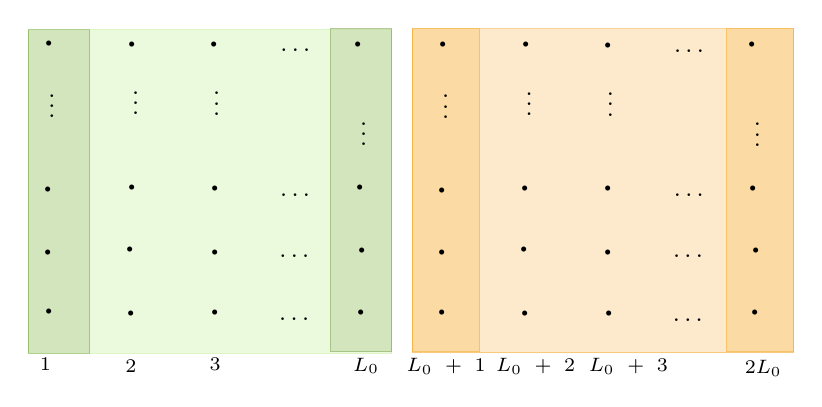
\begin{tikzpicture}[x=0.75pt,y=0.75pt,yscale=-1,xscale=1]
%uncomment if require: \path (0,300); %set diagram left start at 0, and has height of 300

%Shape: Rectangle [id:dp3848625804971728] 
\draw  [color={rgb, 255:red, 184; green, 233; blue, 134 }  ,draw opacity=0.46 ][fill={rgb, 255:red, 184; green, 233; blue, 134 }  ,fill opacity=0.28 ] (234.89,30) -- (410.03,30) -- (410.03,185.94) -- (234.89,185.94) -- cycle ;
%Shape: Rectangle [id:dp9450776254434018] 
\draw  [color={rgb, 255:red, 65; green, 117; blue, 5 }  ,draw opacity=0.29 ][fill={rgb, 255:red, 65; green, 117; blue, 5 }  ,fill opacity=0.15 ] (380.36,29.33) -- (410.03,29.33) -- (410.03,185.28) -- (380.36,185.28) -- cycle ;
%Shape: Rectangle [id:dp43101617233074474] 
\draw  [color={rgb, 255:red, 245; green, 166; blue, 35 }  ,draw opacity=0.47 ][fill={rgb, 255:red, 245; green, 166; blue, 35 }  ,fill opacity=0.23 ] (419.89,29.67) -- (603.69,29.67) -- (603.69,185.61) -- (419.89,185.61) -- cycle ;
%Shape: Rectangle [id:dp31365082950207435] 
\draw  [color={rgb, 255:red, 245; green, 166; blue, 35 }  ,draw opacity=0.46 ][fill={rgb, 255:red, 245; green, 166; blue, 35 }  ,fill opacity=0.24 ] (419.89,29.67) -- (452.36,29.67) -- (452.36,185.28) -- (419.89,185.28) -- cycle ;
%Shape: Rectangle [id:dp8808840272817517] 
\draw  [color={rgb, 255:red, 65; green, 117; blue, 5 }  ,draw opacity=0.29 ][fill={rgb, 255:red, 65; green, 117; blue, 5 }  ,fill opacity=0.15 ] (234.89,30) -- (264.56,30) -- (264.56,185.94) -- (234.89,185.94) -- cycle ;
%Shape: Rectangle [id:dp5267719982198491] 
\draw  [color={rgb, 255:red, 245; green, 166; blue, 35 }  ,draw opacity=0.46 ][fill={rgb, 255:red, 245; green, 166; blue, 35 }  ,fill opacity=0.24 ] (571.22,29.67) -- (603.69,29.67) -- (603.69,185.28) -- (571.22,185.28) -- cycle ;

% Text Node
\draw (240.42,31.05) node [anchor=north west][inner sep=0.75pt]  [font=\LARGE]  {$\cdot $};
% Text Node
\draw (243.37,52.51) node [anchor=north west][inner sep=0.75pt]  [font=\small]  {$\vdots $};
% Text Node
\draw (240.24,101.21) node [anchor=north west][inner sep=0.75pt]  [font=\LARGE]  {$\cdot $};
% Text Node
\draw (240.24,131.49) node [anchor=north west][inner sep=0.75pt]  [font=\LARGE]  {$\cdot $};
% Text Node
\draw (240.28,160.21) node [anchor=north west][inner sep=0.75pt]  [font=\LARGE]  {$\cdot $};
% Text Node
\draw (280.68,31.27) node [anchor=north west][inner sep=0.75pt]  [font=\LARGE]  {$\cdot $};
% Text Node
\draw (283.63,51.3) node [anchor=north west][inner sep=0.75pt]  [font=\small]  {$\vdots $};
% Text Node
\draw (280.36,100.29) node [anchor=north west][inner sep=0.75pt]  [font=\LARGE]  {$\cdot $};
% Text Node
\draw (279.76,130.1) node [anchor=north west][inner sep=0.75pt]  [font=\LARGE]  {$\cdot $};
% Text Node
\draw (280.11,160.87) node [anchor=north west][inner sep=0.75pt]  [font=\LARGE]  {$\cdot $};
% Text Node
\draw (320.17,31.67) node [anchor=north west][inner sep=0.75pt]  [font=\LARGE]  {$\cdot $};
% Text Node
\draw (322.72,51.5) node [anchor=north west][inner sep=0.75pt]  [font=\small]  {$\vdots $};
% Text Node
\draw (320.25,100.69) node [anchor=north west][inner sep=0.75pt]  [font=\LARGE]  {$\cdot $};
% Text Node
\draw (320.25,131.5) node [anchor=north west][inner sep=0.75pt]  [font=\LARGE]  {$\cdot $};
% Text Node
\draw (320.4,160.47) node [anchor=north west][inner sep=0.75pt]  [font=\LARGE]  {$\cdot $};
% Text Node
\draw (354.56,167.68) node [anchor=north west][inner sep=0.75pt]  [font=\small]  {$\dotsc $};
% Text Node
\draw (354.63,137.09) node [anchor=north west][inner sep=0.75pt]  [font=\small]  {$\dotsc $};
% Text Node
\draw (355.03,107.72) node [anchor=north west][inner sep=0.75pt]  [font=\small]  {$\dotsc $};
% Text Node
\draw (355.13,38.18) node [anchor=north west][inner sep=0.75pt]  [font=\small]  {$\dotsc $};
% Text Node
\draw (389.61,31.23) node [anchor=north west][inner sep=0.75pt]  [font=\LARGE]  {$\cdot $};
% Text Node
\draw (393.57,66.1) node [anchor=north west][inner sep=0.75pt]  [font=\small]  {$\vdots $};
% Text Node
\draw (390.23,100.27) node [anchor=north west][inner sep=0.75pt]  [font=\LARGE]  {$\cdot $};
% Text Node
\draw (391.23,130.48) node [anchor=north west][inner sep=0.75pt]  [font=\LARGE]  {$\cdot $};
% Text Node
\draw (390.85,160.43) node [anchor=north west][inner sep=0.75pt]  [font=\LARGE]  {$\cdot $};
% Text Node
\draw (239.25,186.84) node [anchor=north west][inner sep=0.75pt]  [font=\scriptsize]  {$1$};
% Text Node
\draw (280.45,187.75) node [anchor=north west][inner sep=0.75pt]  [font=\scriptsize]  {$2$};
% Text Node
\draw (321.04,186.77) node [anchor=north west][inner sep=0.75pt]  [font=\scriptsize]  {$3$};
% Text Node
\draw (390.19,186.87) node [anchor=north west][inner sep=0.75pt]  [font=\scriptsize]  {$L_{0}$};
% Text Node
\draw (430.09,31.4) node [anchor=north west][inner sep=0.75pt]  [font=\LARGE]  {$\cdot $};
% Text Node
\draw (433.03,52.87) node [anchor=north west][inner sep=0.75pt]  [font=\small]  {$\vdots $};
% Text Node
\draw (429.91,101.57) node [anchor=north west][inner sep=0.75pt]  [font=\LARGE]  {$\cdot $};
% Text Node
\draw (429.91,131.85) node [anchor=north west][inner sep=0.75pt]  [font=\LARGE]  {$\cdot $};
% Text Node
\draw (429.95,160.56) node [anchor=north west][inner sep=0.75pt]  [font=\LARGE]  {$\cdot $};
% Text Node
\draw (470.35,31.62) node [anchor=north west][inner sep=0.75pt]  [font=\LARGE]  {$\cdot $};
% Text Node
\draw (473.3,51.65) node [anchor=north west][inner sep=0.75pt]  [font=\small]  {$\vdots $};
% Text Node
\draw (470.03,100.65) node [anchor=north west][inner sep=0.75pt]  [font=\LARGE]  {$\cdot $};
% Text Node
\draw (469.43,130.45) node [anchor=north west][inner sep=0.75pt]  [font=\LARGE]  {$\cdot $};
% Text Node
\draw (469.78,161.22) node [anchor=north west][inner sep=0.75pt]  [font=\LARGE]  {$\cdot $};
% Text Node
\draw (509.83,32.02) node [anchor=north west][inner sep=0.75pt]  [font=\LARGE]  {$\cdot $};
% Text Node
\draw (512.38,51.85) node [anchor=north west][inner sep=0.75pt]  [font=\small]  {$\vdots $};
% Text Node
\draw (509.91,101.05) node [anchor=north west][inner sep=0.75pt]  [font=\LARGE]  {$\cdot $};
% Text Node
\draw (509.91,131.85) node [anchor=north west][inner sep=0.75pt]  [font=\LARGE]  {$\cdot $};
% Text Node
\draw (510.07,160.82) node [anchor=north west][inner sep=0.75pt]  [font=\LARGE]  {$\cdot $};
% Text Node
\draw (544.23,168.03) node [anchor=north west][inner sep=0.75pt]  [font=\small]  {$\dotsc $};
% Text Node
\draw (544.3,137.45) node [anchor=north west][inner sep=0.75pt]  [font=\small]  {$\dotsc $};
% Text Node
\draw (544.7,108.08) node [anchor=north west][inner sep=0.75pt]  [font=\small]  {$\dotsc $};
% Text Node
\draw (544.79,38.53) node [anchor=north west][inner sep=0.75pt]  [font=\small]  {$\dotsc $};
% Text Node
\draw (579.28,31.58) node [anchor=north west][inner sep=0.75pt]  [font=\LARGE]  {$\cdot $};
% Text Node
\draw (583.24,66.45) node [anchor=north west][inner sep=0.75pt]  [font=\small]  {$\vdots $};
% Text Node
\draw (579.9,100.62) node [anchor=north west][inner sep=0.75pt]  [font=\LARGE]  {$\cdot $};
% Text Node
\draw (580.9,130.83) node [anchor=north west][inner sep=0.75pt]  [font=\LARGE]  {$\cdot $};
% Text Node
\draw (580.52,160.78) node [anchor=north west][inner sep=0.75pt]  [font=\LARGE]  {$\cdot $};
% Text Node
\draw (415.92,187.2) node [anchor=north west][inner sep=0.75pt]  [font=\scriptsize]  {$L_{0} \ +\ 1$};
% Text Node
\draw (459.11,187.1) node [anchor=north west][inner sep=0.75pt]  [font=\scriptsize]  {$L_{0} \ +\ 2$};
% Text Node
\draw (503.71,187.13) node [anchor=north west][inner sep=0.75pt]  [font=\scriptsize]  {$L_{0} \ +\ 3$};
% Text Node
\draw (578.86,188.22) node [anchor=north west][inner sep=0.75pt]  [font=\scriptsize]  {$2L_{0}$};


\end{tikzpicture}

    \caption{Lattice decomposition for the case of periodic boundary conditions. We split the system into two parts, each one has two borders (darker regions). The last time slice $2L_0$ is connected to the first one $1$.}
    \label{fig: fig p bc}
\end{figure}
\\ Using the Schur decomposition \eqref{Schur}, we can write the determinant as:
\begin{equation}
    \det(\mathcal{D}) = \det(B) \det \left[ \begin{pmatrix}
        A & F_2 & \mathbb{0} \\
        F_2' & C & F_3 \\
        \mathbb{0} & F_3' & D
    \end{pmatrix} - \begin{pmatrix}
        F_1' \\
        \mathbb{0} \\
        \mathbb{0} \\
    \end{pmatrix} B^{-1} \begin{pmatrix}
        F_1 & \mathbb{0} & \mathbb{0} \\
    \end{pmatrix}\right]
\end{equation}
If we carry out explicitly the contraction on the last term in the RHS and make use again of the Schur decomposition, we can write:
\begin{equation}\label{decomp pre-M}
    \begin{split}
        \det (\mathcal{D}) &= \det (B) \det \begin{pmatrix}
            A - F_1' B^{-1} F_1 & F_2 & \mathbb{0} \\
            F_2' & C & F_3 \\
            \mathbb{0} & F_3' & D \\
        \end{pmatrix} \\
        &= \det (B) \det (D) \det \begin{pmatrix}
            A - F_1' B^{-1} F_1 & F_2 \\
            F_2' & C - F_3 D^{-1} F_3'
        \end{pmatrix}
    \end{split}
\end{equation}
Given the previous expressions, we have to deal also with the inverse matrices $B^{-1}$ and $D^{-1}$ in order to compute $F_1' B^{-1} F_1$ and $F_3 D^{-1} F_3'$. They can be written in a block-matrix form, and we just need to focus on the $2L_1 \cross 2L_1$ blocks which lie on the corners, namely:
\begin{equation}
    B^{-1} = \begin{pmatrix}
        B_1^{-1} & \dots & B_2^{-1} \\
        \vdots & & \vdots \\
        B_3^{-1} & \dots & B_4^{-1} \\
    \end{pmatrix} \hspace{5mm} D^{-1} = \begin{pmatrix}
        D_1^{-1} & \dots & D_2^{-1} \\
        \vdots & & \vdots \\
        D_3^{-1} & \dots & D_4^{-1} \\
    \end{pmatrix} \
\end{equation}
Notice that it is not necessary to evaluate the full matrices $B^{-1}$ and $D^{-1}$ to find a single block, since we can recursively make use of the relation:
\begin{equation}
    \begin{pmatrix}
        A & B \\
        C & D \\
    \end{pmatrix}^{-1} = \begin{pmatrix}
        \dots & \dots \\
        \dots & (D - CA^{-1}B)^{-1}
    \end{pmatrix} = \begin{pmatrix}
        (A - BD^{-1}C)^{-1} & \dots \\
        \dots & \dots \\
    \end{pmatrix}
\end{equation}
Each block $B_k^{-1}$ and $D_k^{-1}$ can then be decomposed in $L_1 \cross L_1$ blocks:
\begin{equation}
    B_k^{-1} = \begin{pmatrix}
        B_{k,1}^{-1} & B_{k,2}^{-1} \\
        B_{k,3}^{-1} & B_{k,4}^{-1} \\
    \end{pmatrix} \hspace{5mm} D^{-1} = \begin{pmatrix}
        D_{k,1}^{-1} & D_{k,2}^{-1} \\
        D_{k,3}^{-1} & D_{k,4}^{-1} \\
    \end{pmatrix} \
\end{equation}
so that we can evaluate the products $F_1' B^{-1} F_1$ and $F_3 D^{-1} F_3'$:
\begin{equation}
    F_1' B^{-1} F_1 = \begin{pmatrix}
        \mathbb{0} & \Lambda_{1,2} B^{-1}_{1,2} \Bar{\Lambda}_{1,2} & \Lambda_{1,2} B^{-1}_{2,1} \Lambda_{L_0 - 1, L_0} & \mathbb{0} \\
        \mathbb{0} & \mathbb{0} & \mathbb{0} & \mathbb{0} \\
        \mathbb{0} & \mathbb{0} & \mathbb{0} & \mathbb{0} \\
        \mathbb{0} & \Bar{\Lambda}_{L_0 - 1, L_0} B_{3,4}^{-1} \Bar{\Lambda}_{1,2} & \Bar{\Lambda}_{L_0 - 1, L_0} B_{4,3}^{-1} \Bar{\Lambda}_{L_0 - 1,L_0} & \mathbb{0} \\
    \end{pmatrix}
\end{equation}
\begin{equation}
    F_3' D^{-1} F_3 = \begin{pmatrix}
        \mathbb{0} & \mathbb{0} & \mathbb{0} & \mathbb{0} \\
        \Bar{\Lambda}_{2L_0 - 1, 2L_0} D_{4,3}^{-1} \Bar{\Lambda}_{2L_0 - 1, 2L_0}  & \mathbb{0} & \mathbb{0} & \Bar{\Lambda}_{2L_0 - 1, 2L_0} D_{3,4}^{-1} \Bar{\Lambda}_{L_0 + 1, L_0 + 2} \\
        \Lambda_{L_0 + 1, L_0 + 2} D^{-1}_{2,1} \Lambda_{2L_0 - 1, 2L_0} & \mathbb{0} & \mathbb{0} & \Lambda_{L_0 + 1, L_0 + 2} D^{-1}_{1,2} \Bar{\Lambda}_{L_0 + 1, L_0 + 2} \\
        \mathbb{0} & \mathbb{0} & \mathbb{0} & \mathbb{0} \\
    \end{pmatrix}
\end{equation}
Given the previous definitions, it follows immediately that:
\begin{equation}
\begin{split}
    &A - F_1' B^{-1} F_1 = \begin{pmatrix}
        X_1 & \Tilde{Y}_1 & \Tilde{\Lambda}_{1, L_0} & \mathbb{0} \\
        Y_1 & X_1 & \mathbb{0} & \mathbb{0} \\
        \mathbb{0} & \mathbb{0} & X_{L_0} & Y_{L_0} \\
        \mathbb{0} & \Tilde{\Lambda}_{L_0, 1} & \Tilde{Y}_{L_0} & X_{L_0} \\
    \end{pmatrix} \\ &C - F_3' D^{-1} F_3 = \begin{pmatrix}
        X_{2L_0} & Y_{2L_0} & \mathbb{0} & \mathbb{0} \\
        \Tilde{Y}_{2L_0} & X_{2L_0} & \mathbb{0} & \Tilde{\Lambda}_{2L_0, L_0 + 1} \\
        \Tilde{\Lambda}_{L_0 + 1, 2L_0} & \mathbb{0} & X_{L_0 + 1} & \Tilde{Y}_{L_0 + 1} \\
        \mathbb{0} & \mathbb{0} & Y_{L_0 + 1} & X_{L_0 + 1} \\
    \end{pmatrix}
    \end{split}
\end{equation}
where we introduced:
\begin{equation}
    \begin{split}
       & \Tilde{Y}_1 = Y_1 - \Lambda_{1,2} B^{-1}_{1,2} \Bar{\Lambda}_{1,2} \\
       & \Tilde{Y}_{L_0} = Y_{L_0} - \Bar{\Lambda}_{L_0 - 1,L_0} B^{-1}_{4,3} \Lambda_{L_0 - 1, L_0} \\
       & \Tilde{Y}_{L_0 + 1} = Y_{L_0 + 1} - \Lambda_{L_0 + 1,L_0 + 2} D^{-1}_{1,2} \Bar{\Lambda}_{L_0 + 1,L_0 + 2} \\
       & \Tilde{Y}_{2L_0} = Y_{2L_0} - \Bar{\Lambda}_{2L_0 - 1,2L_0} D^{-1}_{4,3} \Lambda_{2L_0 - 1, 2L_0} \\
       & \Tilde{\Lambda}_{1, L_0} = - \Lambda_{1,2} B^{-1}_{2,1} \Lambda_{L_0 - 1, L_0} \\
       & \Tilde{\Lambda}_{L_0, 1} = - \Bar{\Lambda}_{L_0 - 1, L_0} B_{3,4}^{-1} \Bar{\Lambda}_{1,2} \\
       & \Tilde{\Lambda}_{2L_0, L_0 + 1} = - \Bar{\Lambda}_{2L_0 - 1, 2L_0} D_{3,4}^{-1} \Bar{\Lambda}_{L_0 + 1, L_0 + 2} \\
       & \Tilde{\Lambda}_{L_0 + 1, L_0 + 2} = -  \Lambda_{L_0 + 1, L_0 + 2} D^{-1}_{2,1} \Lambda_{2L_0 - 1, 2L_0}
    \end{split}
\end{equation}
Hence we can rewrite the last matrix on the RHS of \eqref{decomp pre-M} as:
\begin{equation}
    \mathcal{M} = \begin{pmatrix}
         X_1 & \Tilde{Y}_1 & \Tilde{\Lambda}_{1, L_0} & \mathbb{0}  & \mathbb{0}  & \mathbb{0} & \mathbb{0}  \\
        Y_1 & X_1 & \mathbb{0} & \mathbb{0}  & \mathbb{0} & \Bar{\Lambda}_{2L_0, 1} & \mathbb{0}  & \mathbb{0} \\
        \mathbb{0} & \mathbb{0} & X_{L_0} & Y_{L_0}  & \mathbb{0}  & \mathbb{0} & \Lambda_{L_0, L_0 + 1}  & \mathbb{0} \\
        \mathbb{0} & \Tilde{\Lambda}_{L_0, 1} & \Tilde{Y}_{L_0} & X_{L_0}  & \mathbb{0}  & \mathbb{0} & \mathbb{0}  & \mathbb{0} \\
        \Lambda_{2L_0, 1} & \mathbb{0} & \mathbb{0} & \mathbb{0} & X_{2L_0} & Y_{2L_0} & \mathbb{0} & \mathbb{0} \\
        \mathbb{0} & \mathbb{0} & \mathbb{0} & \mathbb{0} & \Tilde{Y}_{2L_0} & X_{2L_0} & \mathbb{0} & \Tilde{\Lambda}_{2L_0, L_0 + 1} \\
        \mathbb{0} & \mathbb{0} & \mathbb{0} & \mathbb{0} & \Tilde{\Lambda}_{L_0 + 1, 2L_0} & \mathbb{0} & X_{L_0 + 1} & \Tilde{Y}_{L_0 + 1} \\
        \mathbb{0} & \mathbb{0} & \mathbb{0} & \Bar{\Lambda}_{L_0, L_0 + 1} & \mathbb{0} & \mathbb{0} & Y_{L_0 + 1} & X_{L_0 + 1} \\
    \end{pmatrix}
\end{equation}
and \eqref{decomp pre-M} becomes:
\begin{equation}
    \det(\mathcal{D}) = \det(B) \det(D) \det(\mathcal{M})
\end{equation}
It is now convenient to perform some rotations which leave $\det(\mathcal{M})$ invariant: by swapping rows and columns $(2 \leftrightarrow 4)$ and $(6 \leftrightarrow 8)$ and by recasting the resulting blocks similarly to what we did in \eqref{rot}, we get the matrix:
\begin{equation}
    \mathcal{M} = \begin{pmatrix}
         \mathbb{0} & \mathbb{0} & \Tilde{\Lambda}_{1, L_0} & \Tilde{Y}_1 & X_1  \mathbb{0}  & \mathbb{0} & \mathbb{0}  \\
        \mathbb{0} & \mathbb{0} & \Tilde{Y}_{L_0} & \Tilde{\Lambda}_{L_0, 1}  & \mathbb{0} & X_{L_0} & \mathbb{0}  & \mathbb{0} \\
        \Tilde{\Lambda}_{L_0 + 1, 2L_0} & \Tilde{Y}_{L_0 + 1} & \mathbb{0} & \mathbb{0}  & \mathbb{0} & \mathbb{0} & X_{L_0 + 1}  & \mathbb{0} \\
        \Tilde{Y}_{2L_0} &  \Tilde{\Lambda}_{2L_0, L_0 + 1} & \mathbb{0} & \mathbb{0} & \mathbb{0} & \mathbb{0} & \mathbb{0} & X_{2L_0} \\
        X_{2L_0} & \mathbb{0} & \mathbb{0} & \mathbb{0} & \Lambda_{2L_0, 1} & \mathbb{0} & \mathbb{0} & \mathbb{0} \\
        \mathbb{0} & X_{L_0 + 1} & \mathbb{0} & \mathbb{0} & \mathbb{0} & \Bar{\Lambda}_{L_0, L_0 + 1} & Y_{L_0 + 1} & \mathbb{0} \\
        \mathbb{0} & \mathbb{0} & X_{L_0} & \mathbb{0} & \mathbb{0} & Y_{L_0} & \Lambda_{L_0, L_0 + 1} & \mathbb{0} \\
        \mathbb{0} & \mathbb{0} & \mathbb{0} & X_1 & Y_1 & \mathbb{0} & \mathbb{0} & \Bar{\Lambda}_{2L_0, 1} \\
    \end{pmatrix}
\end{equation}
and since we will need to refer to some portions of this matrix, we can label its blocks as:
\begin{equation}
    \mathcal{M} = \begin{pmatrix}
        \mathcal{M}_{1,1} &  \mathcal{M}_{1,2} \\ 
         \mathcal{M}_{2,1} &  \mathcal{M}_{2,2} \\
    \end{pmatrix} \hspace{2mm} \Dot{Y}_{1, L_0} = \begin{pmatrix}
        \Tilde{\Lambda}_{1, L_0} & \Tilde{Y}_1 \\
        \Tilde{Y}_{L_0} & \Tilde{\Lambda}_{L_0, 1} \\
    \end{pmatrix} \hspace{2mm} \Dot{Y}_{L_0 + 1, 2L_0} = \begin{pmatrix}
        \Tilde{\Lambda}_{L_0 + 1, 2L_0} & \Tilde{Y}_{L_0 + 1} \\
        \Tilde{Y}_{2L_0} & \Tilde{\Lambda}_{2L_0, L_0 + 1} \\
    \end{pmatrix}
\end{equation}
Now we can use the usual Schur decomposition to write:
\begin{equation}\label{det M pbc}
    \det(\mathcal{M}) = \det(\Dot{Y}_{1, L_0}) \det(\Dot{Y}_{L_0 + 1, 2L_0}) \det\left[\mathcal{M}_{2,2} - \mathcal{M}_{2,1} \begin{pmatrix}
        \mathbb{0} & (\Dot{Y}_{L_0 + 1, 2L_0})^{-1} \\
        (\Dot{Y}_{1, L_0})^{-1} & \mathbb{0} \\
    \end{pmatrix} \mathcal{M}_{1,2} \right] 
\end{equation}
The last determinant in the RHS needs to be factorized, hence it is useful to define the matrix:
\begin{equation}
    \Tilde{d} = \begin{pmatrix}
        \Lambda_{2L_0, 1} & \mathbb{0} & (\hat{Y}_{L_0 + 1, 2L_0})_{1,1} & (\hat{Y}_{L_0 + 1, 2L_0})_{1,2} \\
        \mathbb{0} & \Bar{\Lambda}_{L_0, L_0 + 1} & (\hat{Y}_{L_0 + 1, 2L_0})_{2,1} & (\hat{Y}_{L_0 + 1, 2L_0})_{2,2} \\
        (\hat{Y}_{1, L_0})_{1,1} & (\hat{Y}_{1, L_0})_{1,2} & \Lambda_{L_0, L_0 + 1} & \mathbb{0} \\
        (\hat{Y}_{1, L_0})_{2,1} & (\hat{Y}_{1, L_0})_{2,2} & \mathbb{0} & \Bar{\Lambda}_{2L_0, 1}
    \end{pmatrix}
\end{equation}
where $(\hat{Y}_{\dots})_{i, j}$ denote the blocks of the following matrices of dimensions $2L_1 \cross 2L_1$:
\begin{equation}
    \begin{split}
        & \hat{Y}_{1, L_0} = \begin{pmatrix}
            \mathbb{0} & Y_{L_0} \\
            Y_1 & \mathbb{0} \\
        \end{pmatrix} - \begin{pmatrix}
            X_{L_0} & \mathbb{0} \\ 
            \mathbb{0} & X_{1} \\
        \end{pmatrix} (\Dot{Y}_{1, L_0})^{-1} \begin{pmatrix}
            X_1 & \mathbb{0} \\
            \mathbb{0} & X_{L_0} \\
        \end{pmatrix} \\
        & \hat{Y}_{L_0 + 1, 2L_0} = \begin{pmatrix}
            \mathbb{0} & Y_{2L_0} \\
            Y_{L_0 + 1} & \mathbb{0} \\
        \end{pmatrix} - \begin{pmatrix}
            X_{2L_0} & \mathbb{0} \\ 
            \mathbb{0} & X_{L_0 + 1} \\
        \end{pmatrix} (\Dot{Y}_{L_0 + 1, 2L_0})^{-1} \begin{pmatrix}
            X_{L_0 + 1} & \mathbb{0} \\
            \mathbb{0} & X_{2L_0} \\
        \end{pmatrix}
    \end{split}
\end{equation}
It is now convenient to perform a rotation that leaves the determinant of $\Tilde{d}$ invariant (hence we will still call the result of the rotation $\Tilde{d})$:
\begin{equation}
\begin{split}
        \Tilde{d} \to & \begin{pmatrix}
            \mathbb{0} & \mathbb{0} & \mathbb{0} & \mathbb{1} \\
            \mathbb{0} & \mathbb{0} & \mathbb{1} & \mathbb{0} \\
            \mathbb{1} & \mathbb{0} & \mathbb{0} & \mathbb{0} \\
            \mathbb{0} & \mathbb{1} & \mathbb{0} & \mathbb{0} \\
        \end{pmatrix} \Tilde{d} \begin{pmatrix}
            \mathbb{0} & \mathbb{0} & \mathbb{1} & \mathbb{0} \\
            \mathbb{0} & \mathbb{0} & \mathbb{0} & \mathbb{1} \\
            \mathbb{0} & \mathbb{1} & \mathbb{0} & \mathbb{0} \\
            \mathbb{1} & \mathbb{0} & \mathbb{0} & \mathbb{0} \\
        \end{pmatrix} = \\ &= \begin{pmatrix}
        \Bar{\Lambda}_{2L_0, 1} & \mathbb{0} & (\hat{Y}'_{1, L_0})_{1,1} & (\hat{Y}'_{1, L_0})_{1,2} \\
        \mathbb{0} & \Lambda_{L_0, L_0 + 1} & (\hat{Y}'_{1, L_0})_{2,1} & (\hat{Y}'_{1, L_0})_{2,2} \\
        (\hat{Y}'_{L_0 + 1, 2L_0})_{1,1} & (\hat{Y}'_{L_0 + 1, 2L_0})_{1,2} & \Lambda_{2L_0, 1} & \mathbb{0} \\
        (\hat{Y}'_{L_0 + 1, 2L_0})_{2,1} & (\hat{Y}'_{L_0 + 1, 2L_0})_{2,2} & \mathbb{0} & \Bar{\Lambda}_{L_0, L_0 + 1}
    \end{pmatrix}
    \end{split}
\end{equation}
Where now the $\hat{Y}'$ matrices are given by:
\begin{equation}
    \Hat{Y}'_{1, L_0} = \begin{pmatrix}
        Y_{1} & \mathbb{0} \\
        \mathbb{0} & Y_{L_0}
    \end{pmatrix} - \begin{pmatrix}
        \mathbb{0} & X_1 \\
        X_{L_0} &  \mathbb{0} \\
    \end{pmatrix} (\Dot{Y}_{1, L_0})^{-1} \begin{pmatrix}
        X_1 & \mathbb{0} \\
        \mathbb{0} & X_{L_0} \\
    \end{pmatrix}
\end{equation}
\begin{equation}
    \Hat{Y}'_{L_0 + 1, 2L_0} = \begin{pmatrix}
        Y_{2L_0} & \mathbb{0} \\
        \mathbb{0} & Y_{L_0 + 1}
    \end{pmatrix} - \begin{pmatrix}
        X_{2L_0} & \mathbb{0} \\
        \mathbb{0} & X_{L_0 + 1} \\
    \end{pmatrix} (\Dot{Y}_{L_0 + 1, 2L_0})^{-1} \begin{pmatrix}
        \mathbb{0} & X_{L_0 + 1} \\
        X_{2L_0} & \mathbb{0}
    \end{pmatrix}
\end{equation}
Analogously to the case of open boundary conditions, we can define the square roots of $\Lambda_{i,j}$:
\begin{equation}
    \lambda_{L_0, L_0 + 1} = \sqrt{\Lambda_{L_0, L_0 + 1}} \hspace{4mm} \Bar{\lambda}_{2L_0, 1} = \sqrt{\Bar{\Lambda}_{2L_0, 1}} \longrightarrow \lambda_i \Bar{\lambda}_i = \mathbb{1}
\end{equation}
so that we can implement a transformation which leaves $\det(\Tilde{d})$ invariant:
\begin{equation}
        \begin{pmatrix}
        i\lambda_{2L_0, 1} & \mathbb{0} & \mathbb{0} & \mathbb{0} \\
        \mathbb{0} & \Bar{\lambda}_{L_0, L_0 + 1} & \mathbb{0} & \mathbb{0} \\
        \mathbb{0} & \mathbb{0} & -i\Bar{\lambda}_{2L_0, 1} & \mathbb{0} \\
        \mathbb{0} & \mathbb{0} & \mathbb{0} & \lambda_{L_0, L_0 + 1} \\
    \end{pmatrix} \Tilde{d} \begin{pmatrix}
        -i\lambda_{2L_0, 1} & \mathbb{0} & \mathbb{0} & \mathbb{0} \\
        \mathbb{0} & \bar{\lambda}_{L_0, L_0 + 1} & \mathbb{0} & \mathbb{0} \\
        \mathbb{0} & \mathbb{0} & i\Bar{\lambda}_{2L_0, 1} & \mathbb{0} \\
        \mathbb{0} & \mathbb{0} & \mathbb{0} & \lambda_{L_0, L_0 + 1} \\
    \end{pmatrix}
\end{equation}
For the sake of clarity, as the determinant does not change, we can still call the result $\Tilde{d}$:
\begin{equation}\label{tilde d}
    \Tilde{d} = \begin{pmatrix}
        \mathbb{1} & \accentset{\ast}{Y}_{1, L_0} \\
        \accentset{\ast}{Y}_{L_0 + 1, 2L_0} & \mathbb{1} \\
    \end{pmatrix}
\end{equation}
where $\accentset{\ast}{Y}_{1, L_0}$ and $\accentset{\ast}{Y}_{L_0 + 1, 2L_0}$ are anti-Hermitian matrices defined by:
\begin{equation}
    \begin{split}
        & \accentset{\ast}{Y}_{1, L_0} = \begin{pmatrix}
            i\lambda_{2L_0, 1} & \mathbb{0} \\
            \mathbb{0} & \bar{\lambda}_{L_0, L_0 + 1}
        \end{pmatrix} \hat{Y}'_{1, L_0} \begin{pmatrix}
            i\Bar{\lambda}_{2L_0, 1} & \mathbb{0} \\
            \mathbb{0} & \lambda_{L_0, L_0 + 1}
        \end{pmatrix} \\
        & \accentset{\ast}{Y}_{L_0 + 1, 2L_0} = \begin{pmatrix}
            -i\Bar{\lambda}_{2L_0, 1} & \mathbb{0} \\
            \mathbb{0} & \lambda_{L_0, L_0 + 1}
        \end{pmatrix} \hat{Y}'_{L_0 + 1, 2L_0} \begin{pmatrix}
            -i\lambda_{2L_0, 1} & \mathbb{0} \\
            \mathbb{0} & \bar{\lambda}_{2L_0, 1}
        \end{pmatrix}
    \end{split}
\end{equation}
Therefore by putting \eqref{decomp pre-M} and \eqref{det M pbc} together, the determinant of the Dirac operator can be written as:
\begin{equation}\label{det D pbc}
    \det(\mathcal{D}) = \det(\mathcal{D}_{2, L_0 - 1}) \det(\mathcal{D}_{L_0 + 2, 2L_0 - 1}) \det(\Dot{Y}_{1, L_0}) \det(\Dot{Y}_{L_0 + 1, 2L_0}) \det(\Tilde{d})
\end{equation}
and the factorization is complete for all the terms but $\det(\Tilde{d})$. Notice that the procedure for periodic boundary conditions follows closely what we have already seen for open boundary conditions in Section \ref{OpenBC}, but since in this case the domains $[1, L_0]$ and $[L_0 + 1, 2L_0]$ have two borders rather than one, the dimensionality of $\Tilde{d}$ is doubled with respect to the previous study.
Keeping in mind this difference, we can introduce analogous bosonic variables $\{\sigma_i\}_{i = 1\dots 4L_1}$ and reproduce the same steps as in \eqref{Begin Pfaffian}-\eqref{Final Pfaffian}. 
One can show that, constructing the real matrices:
\begin{equation}\label{Initial SA SB}
   \accentset{\ast}{K}_{L_0} = \frac{1}{2}\begin{pmatrix}
        \accentset{\ast}{Y}_{L_0} - \accentset{\ast}{Y}_{1, L_0}^T & -i (\accentset{\ast}{Y}_{1, L_0} + \accentset{\ast}{Y}_{1, L_0}^T) \\
        \\
        i(\accentset{\ast}{Y}_{1, L_0} + \accentset{\ast}{Y}_{1, L_0}^T) & \accentset{\ast}{Y}_{1, L_0} - \accentset{\ast}{Y}_{L_0}^T \\
    \end{pmatrix}
\end{equation}
\begin{equation}
   \accentset{\ast}K_{L_0 + 1} = \frac{1}{2}\begin{pmatrix}
        -\accentset{\ast}{Y}_{L_0 + 1} + \accentset{\ast}{Y}_{L_0 + 1, 2L_0}^T & i (\accentset{\ast}{Y}_{L_0 + 1, 2L_0} + \accentset{\ast}{Y}_{L_0 + 1, 2L_0}^T) \\
        \\
        -i(\accentset{\ast}{Y}_{L_0 + 1, 2L_0} + \accentset{\ast}{Y}_{L_0 + 1, 2L_0}^T) & - \accentset{\ast}{Y}_{L_0 + 1, 2L_0} + \accentset{\ast}{Y}_{L_0 + 1, 2L_0}^T \\
    \end{pmatrix}
\end{equation}
\begin{equation}
    \accentset{\ast}{J}(\sigma) = \begin{pmatrix}
        \sigma_1 & \\
        & \ddots & \\
        \\
        & & & \sigma_{4L_1} \\
    \end{pmatrix}\begin{pmatrix}
        0 & 1 & 1 & \dots \\
        -1 & 0 & 1  \\
        -1 & - 1 & \ddots & \\
        \vdots & \\
        & & & & 0 \\
    \end{pmatrix}
    \begin{pmatrix}
        \sigma_1 & \\
        & \ddots & \\
        \\
        & & & \sigma_{4L_1} \\
    \end{pmatrix}
\end{equation}
the determinant $\det(\Tilde{d})$ can be written as:
\begin{equation}\label{det d tilde pbc}
\begin{split}
\det (\Tilde{d}) = \int \mathcal{D}[\sigma] \left[\mathcal{D}[\chi_A] e^{-\frac{1}{2}\chi_A^T S_A \chi_A} \right] \left[\mathcal{D}[\chi_B] e^{-\frac{1}{2}\chi_B^T S_B \chi_B} \right] \\
        \rightarrow \det(\Tilde{d}) = \int \mathcal{D}[\sigma] \textrm{Pf}(S_A)\textrm{Pf}(S_B) \hspace{25mm}
\end{split}
\end{equation}
where:
\begin{equation}\label{final SA SB}
    S_A = \accentset{\ast}{K}_{L_0} + \accentset{\ast}{J}(\sigma) \hspace{5 mm} S_B = \accentset{\ast}{K}_{L_0 + 1} - \accentset{\ast}{J}(\sigma)
\end{equation}
and since $S_A$ and $S_B$ are real skew-symmetric matrices, their Pfaffian is also real.
\\ Putting \eqref{det D pbc} and \eqref{det d tilde pbc} together:
\begin{equation}
    \det(\mathcal{D}) = \int \mathcal{D}[\sigma] \textrm{Pf}(S_A)\textrm{Pf}(S_B) \det(\mathcal{D}_{1, L_0 - 1}) \det(\mathcal{D}_{L_0 + 1, 2L_0}) \det(\Tilde{Y}_{L_0})  \det(\Tilde{Y}_{L_0 + 1})
\end{equation}
we achieve a full factorization of the fermionic determinant.

\section{Numerical test}
In this section we will give some numerical evidence of the complete factorization of the fermionic determinant.
\\ We performed the following tests embedding anti-periodic boundary conditions in the time direction, since these were the boundary conditions held throughout all the previous simulations, and they can be achieved by following the prescription described in the section for periodic boundary conditions and by adding an additive minus sign to the definitions of the matrices $\Lambda_{2L_0, 1}$ and $\Bar{\Lambda}_{2L_0, 1}$. Taken into account this small modification, we want to check the validity of the relation:
\begin{equation}\label{fact pf}
\begin{split}
\det (\Tilde{d}) = \int \mathcal{D}[\sigma] \left[\mathcal{D}[\chi_A] e^{-\frac{1}{2}\chi_A^T S_A \chi_A} \right] \left[\mathcal{D}[\chi_B] e^{-\frac{1}{2}\chi_B^T S_B \chi_B} \right] \\
        \rightarrow \det(\Tilde{d}) = \int \mathcal{D}[\sigma] \textrm{Pf}(S_A)\textrm{Pf}(S_B) \hspace{25mm}
\end{split}
\end{equation}
where the definition of $\Tilde{d}$ is given in \eqref{tilde d}, while $S_A$ and $S_B$ are defined in \eqref{Initial SA SB}-\eqref{final SA SB}.
\\ As we mentioned in the previous section, we can choose different kind of variables for the bosonic fields $\{\sigma\}_{i = 1, \dots, 4L_1}$, for instance Ising variables $\sigma = \{1, -1\}$ and Gaussianly distributed variables. Since the first ones take value over a finite set of numbers, we can perform an explicit computation of the integral over bosonic fields, which in turn becomes a summation of $2^{4L_1}$ terms.
\\ We performed this computation for lattices of extension $4 \times 8$, $4 \times 16$ and $6 \times 16$ with $\beta = 2$ and $m_0 = 0.2$, and in each case the relation \eqref{fact pf} was satisfied exactly. This proves numerically that with the procedure presented in this document, we can achieve a complete factorization of the fermionic determinant, and in literature this is the first prescription where such a result is obtained. 
Notice that the numerical computation of the Pfaffian was carried out using the MATLAB library presented in \cite{Wimmer_2012}. 
\\ We can give a differ insight of the goodness of our factorization procedure by showing some results where Gaussianly distributed variables were embedded as bosonic fields $\sigma$. Namely, we can introduce an ensemble of $N_{\textrm{sources}}$ sets of variables distributed accordingly to a Gaussian $\mathcal{N}(0,1)$, i.e. each set contains the $4L_1$ bosonic fields $\sigma$. Given a gauge configuration extrapolated from our code, we can use this ensemble to offer a stochastic estimation of the integration over $\sigma$ in the RHS of \eqref{fact pf}, by evaluating the Pfaffians over each set of bosonic fields $\{\sigma\}_{i = 1, \dots, 4L_1}^{n = 1, \dots, N_{\textrm{sources}}}$ and taking the average. 
\\ In Figure \eqref{fig: pfaf 4x8}-\eqref{fig: pfaf 6x16} we compare these estimations, computed with an increasing volume of sources, with the exact computation of $\det(\Tilde{d})$, represented by a horizontal line in each plot.
\begin{figure}
    \centering
    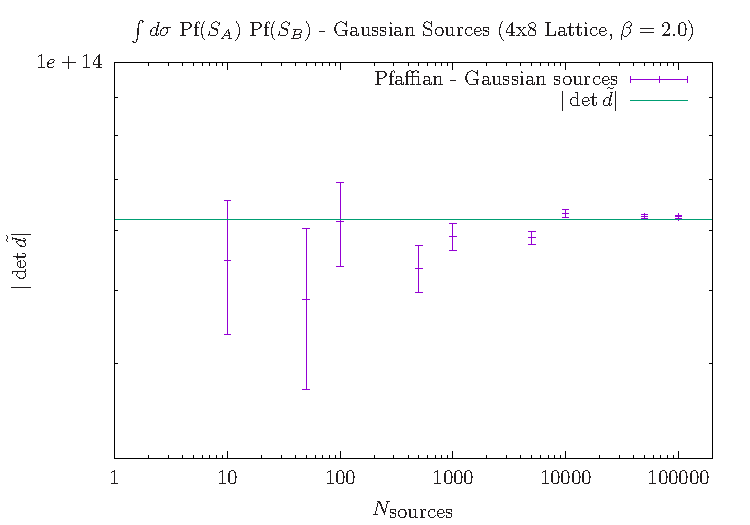
\includegraphics[width=0.8\linewidth]{images/pfaffian4x8.pdf}
    \caption{Numerical test for relation \eqref{fact pf}. This computation was performed on a $4 \times 8$ lattice with $\beta = 2$ and $m_0 = 0.2$.
    The number of sources ranges from 10 to 100000, and the horizontal line represents the value of $\det(\Tilde{d})$.}
    \label{fig: pfaf 4x8}
\end{figure}
\begin{figure}
    \centering
    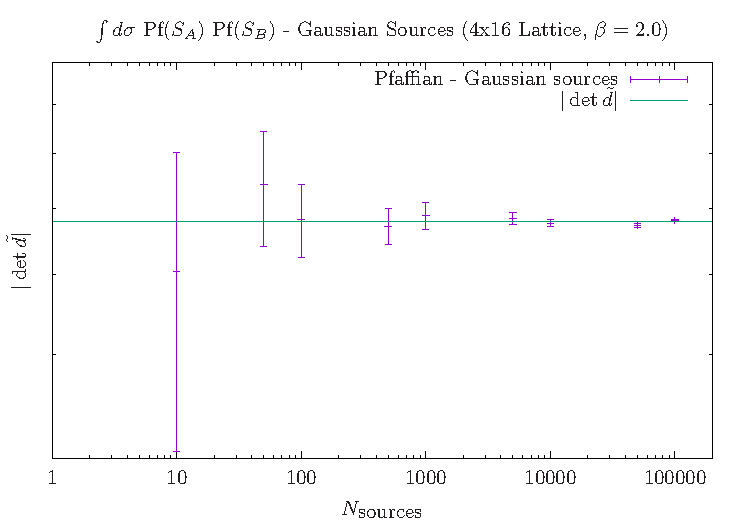
\includegraphics[width=0.8\linewidth]{images/pfaffian4x16.pdf}
    \caption{Numerical test for relation \eqref{fact pf}. This computation was performed on a $4 \times 16$ lattice with $\beta = 2$ and $m_0 = 0.2$.
    The number of sources ranges from 10 to 100000, and the horizontal line represents the value of $\det(\Tilde{d})$.}
    \label{fig: pfaf 4x16}
\end{figure}
\begin{figure}
    \centering
    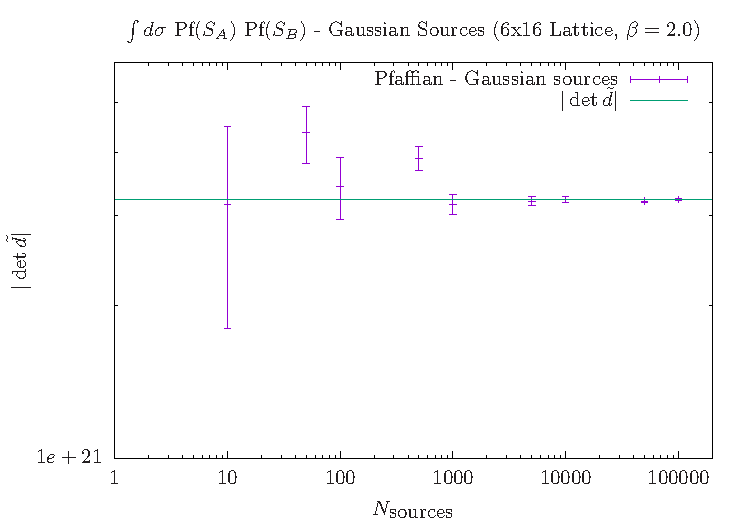
\includegraphics[width=0.8\linewidth]{images/pfaffian6x16.pdf}
    \caption{Numerical test for relation \eqref{fact pf}. This computation was performed on a $6 \times 16$ lattice with $\beta = 2$ and $m_0 = 0.2$.
    The number of sources ranges from 10 to 100000, and the horizontal line represents the value of $\det(\Tilde{d})$.}
    \label{fig: pfaf 6x16}
\end{figure}
Although we performed this tests on small lattices, it is clear that, given a sufficiently large amount of sources, the accordance between $\det(\Tilde{d})$ and the computation employing the Pfaffians is absolutely satisfying also with this stochastic estimation.
\\ These results confirm the goodness of our factorization procedure, which we consider extremely interesting as it allows for a complete separation of the system dynamics and could guarantee a natural factorization of the observables. Indeed the factorization of fermionic observables is the next goal of this research line, as it will allow us to perform deeper analysis about this factorization prescription, in the hope that it actually brings significant improvement in the state of art of lattice computations.
\chapter*{Conclusions and outlook}

The Schwinger Model revealed itself as an instructive framework for several reasons. The design of an Hybrid Monte Carlo algorithm was a good exercise to get acquainted with the numerical challenges one may encounter in Lattice Gauge Theories, and since the algorithm was constructed from scratches, both theoretical and computational aspects have been taken into account. Hadron spectroscopy in QED$_2$ shares several features with QCD$_4$, therefore it was interesting to study the low-lying spectrum of this theory and compare the results with the theoretical predictions. For what concerns the iso-triplet states of the spectrum, the correct approach to chiral limit was successfully retrieved, as the pseudoscalar mass vanished when we drove the fermion mass to zero.
The study of the iso-singlet state, on the other hand, was definitely more challenging, due to fact that its two-point function takes contribution from disconnected Wick contractions, which require way higher computational resources in order to produce accurate data. Nevertheless, we produced valuable results for the correlation function, and also the $\eta$-meson behaviour towards the chiral limit has been roughly confirmed. 
On a broader perspective with respect to this work, deeper analysis may be conducted on this model, as its computational costs are sufficiently low with respect to Lattice QCD.
\\ Despite being somewhat interesting and stimulating by itself, we turned our attention to the Standard Schwinger Model in order to collect some results which could be a useful benchmark for a future algorithm where the new factorization of the fermionic determinant will be employed. The deeper goal of this work is indeed inspired by the perspective of finding new computational methods for Lattice Gauge Theories.
\\ At the state of the art, the current factorization procedure is one of soundest ways to tackle down the exponential problem which affects most computations in Lattice Field Theories, as it paved the way for the implementation of multilevel algorithms for systems with dynamical fermions (there comes the decision to briefly present it here).
\\ Nevertheless, the aim of this work consists in the proposal of a new technique for the factorization of the fermionic determinant, which from our point of view represents something unique in literature, as it is the first procedure where a complete factorization is realized. The decomposition of the lattice in overlapping domains was abandoned in favor of a full block-separation of the system dynamics. The theoretical realization of this procedure is inspired by the fact that the Dirac-Wilson operator can be written as a sparse block matrix, which in turn implies the possibility to exploit algebraic resolution methods to address our problem. Whether in both factorization procedures it is somewhat reasonable to separate most of the contributions to the fermionic determinant into terms which are local in the block fields, only in our proposal the factorization is complete, while the current technique relies on the introduction of multiboson auxiliary fields in order to rewrite the non-local remainder of the quark determinant as a bosonic effective action.
\\ Although one may have preferred to test immediately the effectiveness of this new technique, before we can actually implement it numerically we first need to formalize the factorization of fermionic observables, which nevertheless seems to be rather natural with this prescription and will be the next step in this research line. Consequently, we will have all the necessary ingredients to design multi-level algorithms for systems with dynamical fermions where our new proposal gets implemented.
\\ In order to offer a proper support to the validity of our findings, we tested our factorization prescription numerically, and the positive outcome of these investigations boosts our confidence in the potentiality of this new procedure, even though only some proper computational tests will tell us whether its efficiency is comparable with the current methods in literature.
\appendix
% INCLUSIONE APPENDICI - - PERSONALIZZARE - TENERE COERENTE CON LISTA IN ALTO
\chapter{Detailed Balance Condition}
\label{app:a}
Here we will briefly show that the HMC algorithm satisfies the detailed balance condition\footnote{The proof follows closely what is reported in \cite{Gattringer:2010zz}.}:
\begin{equation}
    T(U'|U) P(U) = T(U|U') P(U')
\end{equation}
Recall that the algorithm embeds two steps: the MD evolution scheme, which offers the proposal for the new configuration, and the accept/reject step. From the first step, we get the value of the transition probability $T(U'|U)$, so we will first focus on the leapfrog evolution scheme. In order to obey the detailed balance condition, a MD trajectory must meet the following requirements:
\begin{itemize}
    \item Area preservation of the integration measure $\mathcal{D}[Q]\mathcal{D}[\pi]$ during the MD evolution;
    \item The trajectory must be \textit{reversible}, hence given two configurations $(\pi,Q)$ and $(\pi', Q')$, we must have $T_{md}(\pi', Q' | \pi, Q) = T_{md}(-\pi, Q| -\pi', Q')$.
\end{itemize}
We want to prove that the leapfrog integration scheme shown above satisfies those conditions. Consider a single evolution step, from Eqs. (\ref{first step pi})-(\ref{first step Q}):
\begin{equation}\label{evolution step}
    \begin{split}
    & \hspace{25mm} Q_0(x) \to Q_1(x) = Q_0(x) + \pi_{\frac{1}{2}}(x) \varepsilon \\
       & \pi_{0}(x) \to \pi_{\frac{1}{2}}(x) =  \pi_{0}(x) - \left. \pdv{S}{Q(x)} \right\rvert_{Q_{0}} \frac{\varepsilon}{2} \to \pi_{1}(x) = \pi_{\frac{1}{2}}(x) - \left. \pdv{S}{Q(x)} \right\rvert_{Q_{1}} \frac{\varepsilon}{2} 
    \end{split}
\end{equation}
where the subscripts label the time steps in units of $\varepsilon$. Area preservation of the measure of integration follows from the fact that the Jacobian associated to this evolution is equal to the identity, indeed:
\begin{equation}
    \det[\frac{\partial(\pi_1, Q_1)}{\partial(\pi_0, Q_0)}] = \det[\frac{\partial(\pi_1, Q_1)}{\partial(\pi_{\frac{1}{2}}, Q_1)}\frac{\partial(\pi_{\frac{1}{2}}, Q_1)}{\partial(\pi_{\frac{1}{2}}, Q_0)}\frac{\partial(\pi_{\frac{1}{2}}, Q_0)}{\partial(\pi_0, Q_0)}]
\end{equation}
Clearly the right-hand side factorizes into three determinants of triangular matrices, e.g.:
\begin{equation}
    \det[\frac{\partial(\pi_{\frac{1}{2}}, Q_0)}{\partial(\pi_0, Q_0)}] = \det\begin{bmatrix}
\,1 & \dots \\
\,0 & 1 
\end{bmatrix} = 1
\end{equation}
Hence the total Jacobian will be equal to 1, and the integration measure is invariant.
\\ For what concerns reversibility, consider a forward step from $(\pi_0, Q_0) \to (\pi_1, Q_1)$, combining the expressions in (\ref{evolution step}) we obtain:
\begin{equation}\label{step final app}
    \begin{split}
    & Q_1(x) = Q_0(x) + \pi_0(x) \varepsilon - \frac{1}{2} \left. \pdv{S}{Q(x)} \right\rvert_{Q_{0}} \varepsilon^2 \\
       & \pi_{1}(x) = \pi_{0}(x) - \frac{1}{2}\left( \left. \pdv{S}{Q(x)} \right\rvert_{Q_{0}} + \left. \pdv{S}{Q(x)} \right\rvert_{Q_{1}} \right) \varepsilon
    \end{split}
\end{equation}
Conversely, if we start at $(\pi_1, Q_1)$ and apply (\ref{evolution step}) with a negative step size $-\varepsilon$, we get a backward step:
\begin{equation}
    \begin{split}
           & Q_1(x) \to Q_1(x) - \pi_1(x) \varepsilon - \frac{1}{2} \left. \pdv{S}{Q(x)} \right\rvert_{Q_{1}} \varepsilon^2 = \\
           & \hspace{10mm} = Q_1(x) - \pi_0(x) \varepsilon + \frac{1}{2}\left( \left. \pdv{S}{Q(x)} \right\rvert_{Q_{0}} + \left. \pdv{S}{Q(x)} \right\rvert_{Q_{1}} \right)  -  \frac{1}{2} \left. \pdv{S}{Q(x)} \right\rvert_{Q_{1}} \varepsilon^2 = \\
           & \hspace{10mm} = Q_1(x) - \pi_0(x) \varepsilon + \frac{1}{2} \left. \pdv{S}{Q(x)} \right\rvert_{Q_{0}} \varepsilon^2 = Q_0(x)  \\
        & \pi_1(x) \to \pi_{1}(x) + \frac{1}{2}\left( \left. \pdv{S}{Q(x)} \right\rvert_{Q_{0}} + \left. \pdv{S}{Q(x)} \right\rvert_{Q_{1}} \right) \varepsilon = \pi_0(x)
    \end{split}
\end{equation}
so we get $(\pi_1, Q_1) \to (\pi_0, Q_0)$, hence reversibility is guaranteed. In the equations of motion, time always multiplies the momenta, so that in the evolution we have indeed $T_{md}(\pi', Q' | \pi, Q) = T_{md}(-\pi, Q| -\pi', Q')$, or equivalently, since $\pi$ enters quadratically in the distributions, $T_{md}(\pi', Q' | \pi, Q) = T_{md}(\pi, Q| \pi', Q')$.
\\ Once that the new configuration has been proposed, since the MD evolution scheme is correct up to $\mathcal{O}(\varepsilon^2)$ discretization errors, we complete the trajectory with a Metropolis step, hence the proposal is accepted only with a probability factor:
\begin{equation}
    T_A(\pi', Q'| \pi, Q) = \min\left(1, \frac{\exp(-H[\pi', Q'])}{\exp(-H[\pi, Q])}\right)
\end{equation}
where $H[\pi, Q] = \frac{\pi^2}{2} + S[Q]$, and this step must satisfy detailed balance. The total probability of transitioning from $Q$ to $Q'$ results from integrating over all momenta:
\begin{equation}\label{T}
    T(Q'|Q) = \int \mathcal{D}[\pi] \mathcal{D}[\pi'] T_A(\pi', Q'|\pi, Q) T_{md} (\pi', Q'| \pi, Q) e^{-\pi^2/2}
\end{equation}
Then we can transform:
\begin{equation}\label{T_A}
    \begin{split}
        T_A(\pi', Q'| \pi, Q) & = \min\left(1, \frac{e^{-\pi'^2/2 - S[Q']}}{e^{-\pi^2/2 - S[Q]}} \right) = \\
        & = \exp(-\frac{\pi'^2}{2} - S[Q'] + \frac{\pi^2}{2} + S[Q]) \min\left(\frac{e^{-\pi^2/2 - S[Q]}}{e^{-\pi'^2/2 - S[Q']}}, 1 \right) = \\ 
        & = \exp(-\frac{\pi'^2}{2} - S[Q'] + \frac{\pi^2}{2} + S[Q]) T_A(\pi, Q!\pi', Q') = \\
        & = \exp(-\frac{\pi'^2}{2} - S[Q'] + \frac{\pi^2}{2} + S[Q]) T_A(-\pi, Q|-\pi', Q')
    \end{split}
\end{equation}
where we used that $T_A$ is even in the momenta in the last step. By using the reversibility of the leapfrog evolution scheme shown above and plugging (\ref{T_A}) into (\ref{T}), the integral becomes:
\begin{equation}
    \begin{split}
        T(Q'|Q) &= \int \mathcal{D}[\pi] \mathcal{D}[\pi'] T_A(-\pi, Q|-\pi', Q') T_{md} (-\pi, Q| -\pi', Q') e^{-S[Q'] + S[Q] -\pi'^2/2} \\ 
        &= \int \mathcal{D}[\pi] \mathcal{D}[\pi'] T_A(\pi, Q|\pi', Q') T_{md} (\pi, Q| \pi', Q') e^{-S[Q'] + S[Q] -\pi'^2/2}
    \end{split}
\end{equation}
where in the second step we changed the sign of all momenta, as the integration measure is invariant under such transformation.
\\ Finally, if we multiply the above expression with $\exp(-S[Q])$ and compare it with (\ref{T}), it is clear that:
\begin{equation}
    \exp(-S[Q]) T(Q'|Q) = \exp(-S[Q']) T(Q|Q')
\end{equation}
which corresponds to the detailed balance condition for the distribution probability of interest. 
\chapter{Drift Force Computation}
\label{app:b}
In this subsection we will compute the driving force of the leapfrog evolution scheme, which is given by:
\begin{equation*}
\begin{split}
    \pdv{S[U]}{Q_0(x)} &= \beta \Im{U_P(x) - U_P(x - \hat{1})} - 2 \Re{\eta^\dagger(y) \left(\pdv{D}{Q_0(x)}D^\dagger\right) (y,z)\, \eta(z)}   \\
    \pdv{S[U]}{Q_1(x)} &= \beta \Im{- U_P(x) + U_P(x - \hat{0})} - 2 \Re{\eta^\dagger(y) \left(\pdv{D}{Q_1(x)}D^\dagger\right) (y,z)\, \eta(z)} 
\end{split}
\end{equation*}
The gauge part is trivial, so we will focus on the second term of the previous expression.
\subsubsection*{Step-by-Step Computation}
Given the definition of $D^\dagger$ in (\ref{D daga}), we can compute: 
\begin{equation}\label{ddagger eta}
\begin{split}
        D^\dagger_{p,n} \eta_n &= \left(D^\dagger \eta \right)_p = \\
        & = \Bar{m} \eta_p - \frac{1}{2}\left[ (1 - \gamma_0) U_0^\dagger(p - \hat{0}) \eta_{p-\hat{0}} + (1 + \gamma_0) U_0 (p) \eta_{p+\hat{0}} \right] - \\
        & \,\,\,\,\,\,\,\,\,\,\, \,\,\,\,\,\,\, \, - \frac{1}{2}\left[ (1 - \gamma_1) U_1^\dagger(p - \hat{1}) \eta_{p-\hat{1}} + (1 + \gamma_1) U_1 (p) \eta_{p + \hat{1}}\right]
\end{split}
\end{equation} 
Then, from the definition of the Dirac operator (\ref{D}), if we update a phase $Q_\mu (k)$ defined at the reticular site $k$ we get:
\begin{equation}\label{deriv D}
    \pdv{D_{m,p}}{Q_\mu(k)} = - \frac{i}{2} \left[ (1 - \gamma_\mu)U_\mu(k) \delta_{m,k} \delta_{p, k + \hat{\mu}} - (1 + \gamma_\mu) U_\mu^\dagger(k)\delta_{m - \hat{\mu}, k} \delta_{p, k}  \right]
\end{equation}
We need to contract this expression with $\eta^\dagger_m$ on the left and $(D^\dagger \eta)_p$ on the right.
For $\mu = 0$:
\begin{equation}\label{force0}
    \begin{split}
        \eta^\dagger \left( \pdv{D}{Q_0(k)} \right) D^\dagger \eta = &- \frac{i}{2} \Bar{m} \left[ \eta^\dagger_k (1 - \gamma_0) U_0 (k) \eta_{k + \hat{0}} - \eta_{k + \hat{0}} (1 + \gamma_0) U_0^\dagger(k)\eta_k \right] + \\
         & + \frac{i}{2} \left[ \eta^\dagger_k (1 - \gamma_0) \eta_k - \eta^\dagger_{k + \hat{0}} (1 + \gamma_0) \eta_{k + \hat{0}} \right] - \\
        & + \frac{i}{4} U_0(k) \eta_k^\dagger \left[ (1-\gamma_0)(1 - \gamma_1) U_1^\dagger(k + \hat{0} - \hat{1}) \eta_{k + \hat{0} -\hat{1}} + \right.  \\ 
        & \,\,\,\,\,\,\,\,\,\,\,\,\,\,\,\,\,\,\,\,\,\,\,\,\,\,\,\,\,\,\,\,\,\,\,\,\, \left. + (1 - \gamma_0)(1 + \gamma_1) U_1 (k + \hat{0}) \eta_{k + \hat{0} + \hat{1}} \right] - \\
        & - \frac{i}{4} U_0^\dagger(k) \eta_{k + \hat{0}}^\dagger \left[(1+\gamma_0)(1 - \gamma_1) U_1^\dagger(k-\hat{1}) \eta_{k - \hat{1}} +  \right. \\
        & \,\,\,\,\,\,\,\,\,\,\,\,\,\,\,\,\,\,\,\,\,\,\,\,\,\,\,\,\,\,\,\,\,\,\,\,\,\,\,\,\,\, \left. + (1 + \gamma_0)(1 + \gamma_1) U_1 (k) \eta_{k + \hat{1}} \right]
    \end{split}
\end{equation}
And finally:
\begin{equation}
    \begin{split}
                2 \Re{\eta^\dagger \left( \pdv{D}{Q_0(k)} \right) D^\dagger \eta} = & \Im \left(\Bar{m} \left[ \eta^\dagger_k (1 - \gamma_0) U_0 (k) \eta_{k + \hat{0}} - \eta^\dagger_{k + \hat{0}} (1 + \gamma_0) U_0^\dagger(k)\eta_k \right] + \right. \\
         & - \left[ \eta^\dagger_k (1 - \gamma_0) \eta_k - \eta^\dagger_{k + \hat{0}} (1 + \gamma_0) \eta_{k + \hat{0}} \right] - \\
        & - \frac{1}{2} U_0(k) \eta_k^\dagger \left[ (1-\gamma_0)(1 - \gamma_1) U_1^\dagger(k + \hat{0} - \hat{1}) \eta_{k + \hat{0} -\hat{1}} + \right.  \\ 
        & \,\,\,\,\,\,\,\,\,\,\,\,\,\,\,\,\,\,\,\,\,\,\,\,\,\,\,\,\,\,\,\,\,\,\,\,\, \left. + (1 - \gamma_0)(1 + \gamma_1) U_1 (k + \hat{0}) \eta_{k + \hat{0} + \hat{1}} \right] - \\
        & + \frac{1}{2} U_0^\dagger(k) \eta_{k + \hat{0}}^\dagger \left[(1+\gamma_0)(1 - \gamma_1) U_1^\dagger(k-\hat{1}) \eta_{k - \hat{1}} +  \right. \\
        & \,\,\,\,\,\,\,\,\,\,\,\,\,\,\,\,\,\,\,\,\,\,\,\,\,\,\,\,\,\,\,\,\,\,\,\,\,\,\,\,\,\, \left. \left. + (1 + \gamma_0)(1 + \gamma_1) U_1 (k) \eta_{k + \hat{1}} \right]\right)
    \end{split}
\end{equation}
After contracting the $\gamma$ matrices, using a notation where $\eta_1(k)$ labels the first component of the pseudofermion $\eta$ defined at the lattice site $k$, we obtain:
\begin{equation}
    \begin{split}
         2 \Re{\eta^\dagger \left( \pdv{D}{Q_0(k)} \right) D^\dagger \eta} = & \Im \left( 2 \Bar{m} \left[U_0 (k) \eta_1^*(k)\eta_1(k + \hat{0}) - U_0^\dagger(k) \eta_2^*(k + \hat{0})\eta_2(k) \right] - \right. \\
         & - 2 \left[ \eta_1^*(k) \eta_1(k) - \eta_2^*(k + \hat{0}) \eta_2(k + \hat{0}) \right] - \\
        & - U_0(k) \eta_1^*(k) \left[ U_1^\dagger(k + \hat{0} - \hat{1}) \eta_-(k + \hat{0} - \hat{1}) + \right.  \\ 
        & \,\,\,\,\,\,\,\,\,\,\,\,\,\,\,\,\,\,\,\,\,\,\,\,\,\,\,\,\,\,\,\,\,\,\,\,\,\,\,\,\,\,\,\, \left. + U_1(k + \hat{0}) \eta_+ (k + \hat{0} + \hat{1}) \right] + \\
        & + U_0^\dagger(k) \eta_{2}^*(k + \hat{0}) \left[ U_1(k) \eta_+ (k + \hat{1}) - U_1^\dagger(k - \hat{1}) \eta_{-}(k - \hat{1})  \right]
    \end{split}
\end{equation}
where:
\begin{equation*}
    \eta_-(k) = \eta_1 (k) - \eta_2(k) \,\,\,\,\,\,\,\,\,\,\, \eta_+(k) = \eta_1 (k) + \eta_2 (k)
\end{equation*}
\\ Analogously, for $\mu = 1$:
\begin{equation}
    \begin{split}
                2 \Re{\eta^\dagger \left( \pdv{D}{Q_1(k)} \right) D^\dagger \eta} = & \Im \left(\Bar{m} \left[ \eta^\dagger_k (1 - \gamma_1) U_1 (k) \eta_{k + \hat{1}} - \eta^\dagger_{k + \hat{1}} (1 + \gamma_1) U_1^\dagger(k)\eta_k \right] + \right. \\
         & -  \left[ \eta^\dagger_k (1 - \gamma_1) \eta_k - \eta^\dagger_{k + \hat{1}} (1 + \gamma_1) \eta_{k + \hat{1}} \right] - \\
        & - \frac{1}{2} U_1(k) \eta_k^\dagger \left[ (1-\gamma_1)(1 - \gamma_0) U_0^\dagger(k + \hat{1} - \hat{0}) \eta_{k + \hat{1} -\hat{0}} + \right.  \\ 
        & \,\,\,\,\,\,\,\,\,\,\,\,\,\,\,\,\,\,\,\,\,\,\,\,\,\,\,\,\,\,\,\,\,\,\,\,\, \left. + (1 - \gamma_1)(1 + \gamma_0) U_0 (k + \hat{1}) \eta_{k + \hat{1} + \hat{0}} \right] - \\
        & + \frac{1}{2} U_1^\dagger(k) \eta_{k + \hat{1}}^\dagger \left[(1+\gamma_1)(1 - \gamma_0) U_0^\dagger(k-\hat{0}) \eta_{k - \hat{0}} +  \right. \\
        & \,\,\,\,\,\,\,\,\,\,\,\,\,\,\,\,\,\,\,\,\,\,\,\,\,\,\,\,\,\,\,\,\,\,\,\,\,\,\,\,\,\, \left. \left. + (1 + \gamma_1)(1 + \gamma_0) U_0 (k) \eta_{k + \hat{0}} \right]\right)
    \end{split}
\end{equation}
and after we use the explicit form of the $\gamma$ matrices:
\begin{equation}
    \begin{split}
         2 \Re{\eta^\dagger \left( \pdv{D}{Q_1(k)} \right) D^\dagger \eta} = & \Im \left( \Bar{m} \left[U_1 (k) \eta_-^*(k)  \eta_-(k + \hat{1}) - U_1^\dagger(k) \eta_+^*(k + \hat{1}) \eta_+(k) \right] - \right. \\
         & -  \left[ \eta_-^*(k) \eta_-(k) - \eta_+^*(k + \hat{1}) \eta_+ (k + \hat{1}) \right] - \\
        & - U_1(k) \eta_-^*(k) \left[ U_0^\dagger ( k + \hat{1} - \hat{0} ) \eta_1 (k + \hat{1} - \hat{0}) - \right.  \\ 
        & \,\,\,\,\,\,\,\,\,\,\,\,\,\,\,\,\,\,\,\,\,\,\,\,\,\,\,\,\,\,\,\,\,\,\,\,\,\,\,\,\,\,\,\, \left. - U_0(k + \hat{1}) \eta_2 (k + \hat{1} + \hat{0}) \right] + \\
        & + U_1^\dagger(k) \eta_{+}^*(k + \hat{1}) \left[ U_0(k) \eta_2 (k + \hat{0}) + U_0^\dagger(k - \hat{0}) \eta_{1}(k - \hat{0})  \right]
    \end{split}
\end{equation}
where:
\begin{equation*}
    \eta_-^*(k) = \eta_1^* (k) - \eta_2^* (k) \,\,\,\,\,\,\,\,\,\,\, \eta_+^*(k) = \eta_1^* (k) + \eta_2^* (k)
\end{equation*}
\vspace{5mm}
\\Alternatively, if we recall that $D^\dagger = \gamma_2 D \gamma_2$, we can write:
\begin{equation*}
    \eta^\dagger \left(\pdv{D D^\dagger}{Q_\mu(k)}\right) \eta = 2 \Re{\eta^\dagger \pdv{\mathcal{D}}{Q_\mu(k)} \mathcal{D}\eta}
\end{equation*}
where $\mathcal{D} = D\gamma_2$. Then it is useful to define:
\begin{equation}
    \psi = \mathcal{D}\eta = D \gamma_2 \eta = D \mqty(-i \eta_2 \\ i \eta_1) = D \eta'
\end{equation}
From (\ref{deriv D}) it is easy to show that:
\begin{equation}\label{deriv Dcal}
    \pdv{\mathcal{D}_{m,p}}{Q_\mu(k)} = - \frac{i}{2} \left[ (1 - \gamma_\mu) \gamma_2 U_\mu(k) \delta_{m,k} \delta_{p, k + \hat{\mu}} - (1 + \gamma_\mu) \gamma_2 U_\mu^\dagger(k)\delta_{m - \hat{\mu}, k} \delta_{p, k}  \right]
\end{equation}
Therefore, we need the contraction:
\begin{equation}
\begin{split}
        \eta^\dagger (m) \pdv{\mathcal{D}_{m,p}}{Q_\mu(k)} \psi(p) =& - \frac{i}{2} \left[\eta^\dagger(k) (1 - \gamma_\mu) \gamma_2 U_\mu(k) \psi(k + \hat{\mu}) \right. \\ & \left. \hspace{20mm} - \eta^\dagger(k + \hat{\mu}) (1 + \gamma_\mu) \gamma_2 U_\mu^\dagger(k) \psi(k)  \right]
\end{split}
\end{equation}
Hence the drift force from the pseudofermion action is:
\begin{equation}
    \begin{split}
        \pdv{S_{pf}}{Q_0(k)} = & - 2 \Re{\eta^\dagger \left( \pdv{\mathcal{D}}{Q_0(k)} \right) \psi} = \\
        = & \Re{i\left[ -2i \eta^*_1(k) U_0(k) \psi_2(k + \hat{0}) - 2i \eta^*_2(k + \hat{0}) U_0^\dagger(k)\psi(k) \right]} = \\
        = & 2 \Re{\eta^*_1(k) U_0(k) \psi_2(k + \hat{0}) + \eta^*_2(k + \hat{0}) U_0^\dagger(k) \psi_1(k)}
    \end{split}
\end{equation}
and analogously: 
\begin{equation}
    \begin{split}
        \pdv{S_{pf}}{Q_1(k)} = & - 2 \Re{\eta^\dagger \left( \pdv{\mathcal{D}}{Q_1(k)} \right) \psi} = \\
        = & \Re\left[-U_1(k) \left[ \left(\eta^*_2(k) - \eta^*_1(k)\right) \left(\psi_1(k + \hat{1}) + \psi_2(k + \hat{1})\right) \right] + \right. \\
        & \hspace{10 mm} + \left. U_1^\dagger(k) \left[ \left( \eta_1^*(k + \hat{1} + \eta_2^*(k + \hat{1}) \right) \left( \psi_1(k) - \psi_2(k) \right) \right] \right]
    \end{split}
\end{equation}

\section{Conjugate Gradient Algorithm}
In order to evaluate the drift force of the time evolution, we need to compute the combination $\eta(x) = (DD^\dagger)^{-1} \phi(x)$, hence we will need an algorithm for matrix inversion. \\ The Conjugate Gradient (CG) algorithm for SPD matrices \cite{Hestenes1952MethodsOC} allows us to find an approximation of the solution $x$ of the linear system $Ax = b$, and in our case $A = DD^{\dagger}$ and $b = \phi$. This algorithm falls into the category of the Krylov Subspaces based techniques, and it consists of the following steps:
\begin{enumerate}
    \item Define an initial guess for $\eta = x$, called $x^{(0)}$, drawn accordingly to a Gaussian distribution.
    \item Compute the initial residual $r^{(0)} = \phi - Ax^{(0)}$ (with $A = DD^\dagger$) and the direction $d^{(0)} = r^{(0)}$. 
    \item Compute iteratively $x^{(k+1)}$, $r^{(k+1)}$, $d^{(k+1)}$, with $k = 0, 1, 2, \dots$ using some two-terms recursion, until the desired accuracy is achieved. In particular:
    \begin{equation}
        x^{(k+1)} = x^{(k)} + \alpha^{(k)}d^{(k)}
    \end{equation}
    where $\alpha^{(k)}$ is a parameter defined as:
    \begin{equation}
        \alpha^{(k)} \equiv \frac{r^{(k)\dagger} r^{(k)}}{d^{(k)\dagger}\, Ad^{(k)}}
    \end{equation}
    Then:
    \begin{equation}
        r^{(k+1)} = r^{(k)} - \alpha^{(k)} Ad^{(k)}
    \end{equation}
    And finally:
    \begin{equation}
        d^{(k+1)} = r^{(k+1)} + \beta^{(k)} d^{(k)}
    \end{equation}
    where $\beta^{(k)}$ is a parameter defined as:
    \begin{equation}
        \beta^{(k)} \equiv \frac{r^{(k+1)\dagger} r^{(k+1)}}{r^{(k)\dagger}\, r^{(k)}}
    \end{equation}
\end{enumerate}
\begin{algorithm}
\caption{ConjugateGradient (pseudo $x$, gauge $u$, pseudo $\phi$)}\label{alg:cap}
\begin{algorithmic}
\State Draw $x$ Gaussian;
\State $r_k = \phi - Ax$;
\State $d = r_k$;
\State Compute residual res = $(r_k, r_k)$;
\While{res $ > \varepsilon $}
\State Compute $Ad$;
\State $\alpha = (r_k, r_k)/(d, Ad)$;
\State $x = x + \alpha \, d$;
\State $r_{k+1} = r_k - \alpha \, Ad$;
\State $\beta = (r_{k+1}, r_{k+1})/(r_k, r_k)$;
\State $d = r_{k+1} + \beta\,d $;
\State Compute residual res = $(r_{k+1}, r_{k+1})$;
\EndWhile
\end{algorithmic}
\end{algorithm}
To embed this algorithm, we need to evaluate $A d^{(k)}$ and $A x^{(0)}$, where $A = DD^{\dagger}$. Since $d^{(k)}$ and $x^{(0)}$ share the same vectorial structure (they are identical to pseudofermion fields), we can build a routine to compute such a contraction.
\subsubsection*{Step-by-Step Computation}
To implement the first step of the algorithm, we need the explicit form of the components of a pseudofermion field $\phi(n)$ defined at the lattice site $n$. It is simply given by the application of the Dirac operator on an auxiliary field $\chi$, which has the same structure as $\phi.$
\begin{equation*}
    \phi(n) = \mqty(\phi_1(n) \\ \phi_2(n)) \hspace{20 mm} \chi(n) = \mqty(\chi_1(n) \\ \chi_2(n))
\end{equation*}
Using the definition in (\ref{D}):
\begin{equation}
\begin{split}
        \phi(m) & = D(m, n) \chi(n) = \\
        & = \Bar{m} \chi(m) - \frac{1}{2} \left[ (1 - \gamma_0)U_0(m) \chi(m + \hat{0}) + (1 + \gamma_0) U_0^\dagger(m - \hat{0}) \chi(m - \hat{0}) \right] - \\
        & - \frac{1}{2} \left[ (1 - \gamma_1)U_1(m) \chi(m + \hat{1}) + (1 + \gamma_1) U_1^\dagger(m - \hat{1}) \chi(m - \hat{1}) \right]
\end{split}
\end{equation}
which gives:
\begin{equation}
    \begin{split}
        \phi_1(m) &= \Bar{m} \chi_1(m) - U_0(m) \chi_1 (m + \hat{0}) - \frac{1}{2} U_1(m) \left( \chi_1(m + \hat{1}) - \chi_2 (m + \hat{1}) \right) - \\
        & - \frac{1}{2} U_1^\dagger(m - \hat{1}) \left( \chi_1 (m - \hat{1}) + \chi_2 (m - \hat{1}) \right)
    \end{split}
\end{equation}
\begin{equation}
    \begin{split}
        \phi_2(m) &= \Bar{m} \chi_2(m) - U_0^\dagger(m - \hat{0}) \chi_2 (m - \hat{0}) - \frac{1}{2} U_1(m) \left( - \chi_1(m + \hat{1}) + \chi_2 (m + \hat{1}) \right) - \\
        & - \frac{1}{2} U_1^\dagger(m - \hat{1}) \left( \chi_1 (m - \hat{1}) + \chi_2 (m - \hat{1}) \right)
    \end{split}
\end{equation}
where $\Bar{m} = m_0 + 2$, and the $\gamma$-matrices are defined in (\ref{gammas}).
\\ Consider now a generic field $d(n)$ defined at the lattice site $n$:
\begin{equation*}
    d(n) = \mqty(d_1(n) \\ d_2(n))
\end{equation*}
If we apply $D^\dagger$ (we understood the fermionic indices $\alpha$ and $\beta$):
\begin{equation}\label{ddagger d}
\begin{split}
        D^\dagger(p,n) d(n) & = \left( \Bar{m} \delta_{n, p} - \frac{1}{2}\left[(1-\gamma_0) U_0^\dagger( p - \hat{0})\delta_{n, p - \hat{0}} + (1 + \gamma_0) U_0 (p) \delta_{n, p + \hat{0}} \right]  - \right. \\ 
        & - \left. \frac{1}{2}\left[(1-\gamma_1) U_1^\dagger(p - \hat{1})\delta_{n, p - \hat{1}} + (1 + \gamma_1) U_1 (p) \delta_{n, p + \hat{1}} \right]   \right) d(n) = \\
        & = \Bar{m}\,d(p) - \frac{1}{2}\left[ (1 - \gamma_0) U_0^\dagger(p - \hat{0})\,d(p-\hat{0}) + (1 + \gamma_0) U_0 (p)\,d(p+\hat{0}) \right] - \\
        & - \frac{1}{2}\left[ (1 - \gamma_1) U_1^\dagger(p - \hat{1})\,d(p-\hat{1}) + (1 + \gamma_1) U_1 (p)\,d(p+\hat{1}) \right]
\end{split}
\end{equation}
Now we can compute the contraction:
\begin{equation*}
    \begin{split}
        D(m, p)(D^\dagger d)(p) =& \left(\Bar{m} \delta_{m,p} - \frac{1}{2}\sum_{\mu} \left[ (1 - \gamma_\mu) U_\mu(m) \delta_{p, m + \hat{\mu}} + (1 + \gamma_\mu) U_\mu^\dagger (m - \mu) \delta_{p, m - \hat{\mu}} \right]\right) \cdot \\
        & \cdot \left( \Bar{m} d(p) - \frac{1}{2}\left[ (1 - \gamma_0) U_0^\dagger(p - \hat{0}) d(p-\hat{0}) + (1 + \gamma_0) U_0 (p) d(p+\hat{0}) \right] - \right. \\ 
        & \hspace{15 mm} \left. - \frac{1}{2}\left[ (1 - \gamma_1) U_1^\dagger(p - \hat{1}) d(p-\hat{1}) + (1 + \gamma_1) U_1 (p) d(p+\hat{1}) \right] \right)
    \end{split}
\end{equation*}
Which can be written as:
\begin{equation*}
        \begin{split}
       & (DD^\dagger d)(m) = \Bar{m}^2 d(m) - \Bar{m}\left[ U_0^\dagger(m - \hat{0}) \mqty(d_1(m-\hat{0}) \\ 0 ) + U_0(m) \mqty(0 \\ d_2(m+\hat{0})) \right] - \\ 
       & \hspace{15 mm} - \frac{1}{2} \Bar{m} \left[ U_1^{\dagger}(m-\hat{1}) \mqty(d_1 (m-\hat{1}) - d_2(m-\hat{1}) \\ - d_1(m-\hat{1}) + d_2 (m-\hat{1}) ) + U_1(m) \mqty( d_1(m + \hat{1})  + d_2(m + \hat{1}) \\ d_1(m + \hat{1})  + d_2(m + \hat{1}) ) \right] \\
       & \hspace{15 mm} - \frac{1}{2} \Gamma_0 - \frac{1}{2}\Gamma_1
        \end{split}
\end{equation*}
with:
\begin{equation*}
    \begin{split}
       \Gamma_0 = & \left( \left[ (1 - \gamma_0) U_0(m) \delta_{p, m+\hat{0}} + (1 + \gamma_0) U_0^\dagger (m - \hat{0}) \delta_{p, m - \hat{0}} \right]\right) \cdot \\
       & \cdot \left( \Bar{m} d(p) - \frac{1}{2}\left[ (1 - \gamma_0) U_0^\dagger(p - \hat{0}) d(p-\hat{0}) + (1 + \gamma_0) U_0 (p) d(p+\hat{0}) \right] - \right. \\ 
       & \left. - \frac{1}{2}\left[ (1 - \gamma_1) U_1^\dagger(p - \hat{1}) d(p-\hat{1}) + (1 + \gamma_1) U_1 (p) d(p+\hat{1}) \right] \right) = \\
       = & \, \Bar{m} \left[ U_0(m)(1 - \gamma_0) d(m+\hat{0}) + U_0^{\dagger}(m - \hat{0}) (1 + \gamma_0) d(m-\hat{0}) \right] + \\
       & - \frac{1}{2} \left[ 2(1 - \gamma_0) U_0(m)U_0^\dagger(m) d(m) + 2(1 + \gamma_0) U_0^\dagger(m-\hat{0}) U_0(m - \hat{0}) d(m) \right] - \\
       & - \frac{1}{2}\left[ (1-\gamma_0)(1-\gamma_1) U_0(m)U_1^\dagger(m+\hat{0}-\hat{1}) d(m+\hat{0} - \hat{1}) + \right. \\ 
       & + (1-\gamma_0)(1 + \gamma_1) U_0(m)U_1(m+\hat{0})d(m+\hat{0}+\hat{1}) +  \\ 
       & + (1+\gamma_0)(1-\gamma_1)U_0^\dagger(m-\hat{0}) U_1^\dagger(m - \hat{0} - \hat{1}) d(m - \hat{0} - \hat{1}) + \\ 
       & + \left. (1+\gamma_0)(1+\gamma_1)U_0^\dagger(m-\hat{0}) U_1(m-\hat{0}) d(m - \hat{0} + \hat{1}) \right]
    \end{split}
\end{equation*}
And analogously: 
\begin{equation*}
    \begin{split}
        \Gamma_1 = & \left( \left[ (1 - \gamma_1) U_1(m) \delta_{p, m+\hat{1}} + (1 + \gamma_1) U_1^\dagger (m - \hat{1}) \delta_{p, m - \hat{1}} \right]\right) \cdot \\
       & \cdot \left( \Bar{m} d(p) - \frac{1}{2}\left[ (1 - \gamma_0) U_0^\dagger(p - \hat{0}) d(p-\hat{0}) + (1 + \gamma_0) U_0 (p) d(p+\hat{0}) \right] - \right. \\ 
       & \left. - \frac{1}{2}\left[ (1 - \gamma_1) U_1^\dagger(p - \hat{1}) d(p-\hat{1}) + (1 + \gamma_1) U_1 (p) d(p+\hat{1}) \right] \right)
    \end{split}
\end{equation*}
Writing explicitly the contraction with the $\gamma$-matrices, we can prove that the components of $\zeta (m) = (DD^\dagger)(m,n) \, d(n)$ are:
\begin{equation*}
    \begin{split}
     \zeta_1(m) &= (\Bar{m}^2 + 2) d_1 (m) - \\
     & - \Bar{m} \left[ U_0^\dagger(m - \hat{0}) d_1(m - \hat{0}) + U_1^\dagger(m - \hat{1}) d_1(m-\hat{1}) + \right. \\ 
     & \hspace{40 mm} \left. + U_1(m) d_1(m + \hat{1}) + U_0 (m) d_1(m + \hat{0})  \right] + \\
     & + U_0 (m) \left[ U_1^\dagger(m + \hat{0} - \hat{1}) d_-(m + \hat{0} - \hat{1}) + U_1(m + \hat{0}) d_+(m + \hat{0} + \hat{1}) \right] + \\ 
     & + \frac{1}{2} U_1 (m) \left[ U_0^\dagger(m + \hat{1} - \hat{0}) d_1(m + \hat{1} - \hat{0}) - U_0(m + \hat{1}) d_2(m + \hat{1} + \hat{0}) \right] +  \\ 
     & + \frac{1}{2} U_1^\dagger (m - \hat{1}) \left[ U_0^\dagger(m - \hat{1} - \hat{0}) d_1(m - \hat{1} - \hat{0}) + U_0(m - \hat{1}) d_2(m - \hat{1} + \hat{0}) \right] \\ 
    \end{split}
\end{equation*}
and: 
\begin{equation*}
    \begin{split}
     \zeta_2(m) &= (\Bar{m}^2 + 2) d_2(m) - \\
     & - \Bar{m} \left[ U_0^\dagger(m - \hat{0}) d_2(m - \hat{0}) + U_1^\dagger(m - \hat{1}) d_2(m-\hat{1}) + \right. \\ 
     & \hspace{40mm} \left. + U_1(m) d_2(m + \hat{1}) + U_0 (m) d_2(m + \hat{0}) \right] + \\
     & + U_0^\dagger (m - \hat{0}) \left[ - U_1^\dagger(m - \hat{0} - \hat{1}) d_-(m - \hat{0} - \hat{1}) + U_1(m - \hat{0}) d_+(m - \hat{0} + \hat{1}) \right] +  \\ 
     & + \frac{1}{2} U_1 (m) \left[ -U_0^\dagger(m + \hat{1} - \hat{0}) d_1(m + \hat{1} - \hat{0}) + U_0(m + \hat{1}) d_2(m + \hat{1} + \hat{0}) \right] +  \\ 
     & + \frac{1}{2} U_1^\dagger (m - \hat{1}) \left[ U_0^\dagger(m - \hat{1} - \hat{0}) d_1(m - \hat{1} - \hat{0}) + U_0(m - \hat{1}) d_2(m - \hat{1} + \hat{0}) \right] +  \\ 
    \end{split}
\end{equation*}
where
\begin{equation*}
    d_-(k) = \frac{d_1 (k) - d_2(k)}{2} \,\,\,\,\,\,\,\,\,\,\, d_+(k) = \frac{d_1 (k) + d_2 (k)}{2}
\end{equation*}
\chapter{$\mathcal{O}(a)$-improved Wilson-Dirac operator}
\label{app: Wilson improved op}

The massive $\mathcal{O}(a)$-improved Wilson-Dirac operator is defined as \cite{L_scher_2013, L_scher_1996, SHEIKHOLESLAMI1985572}:
\begin{equation}\label{dirac improved}
    D = D_{\textrm{w}} + \delta D_{\textrm{v}} + \delta D_{\textrm{b}} + m_0
\end{equation}
where $m_0$ is the bare quark mass, and $D_{\textrm{w}}$ is the massless Wilson-Dirac operator:
\begin{equation}
    D_{\textrm{w}} = \frac{1}{2}\{\gamma_\mu \left(\nabla^*_\mu + \nabla_\mu \right) - \nabla^*_\mu \nabla_\mu\}
\end{equation}
with $\gamma_\mu$ being the Dirac matrices, and the summation over repeated indices is understood.
\\ We define the covariant forward and backward derivatives $\nabla_\mu$ and $\nabla^*_\mu$ as:
\begin{equation}
    \nabla_\mu \psi(x) = U_\mu(x) \psi(x + \hat{\mu}) - \psi(x) \hspace{8mm} \nabla^*_\mu \psi(x) = \psi(x) -  U^\dagger_\mu(x - \hat{\mu}) \psi(x - \hat{\mu}) - \psi(x)
\end{equation}
where $\psi(x)$ is a generic fermion field, $U_\mu(x)$ are the link fields and $\hat{\mu}$ is the unit vector defined along the direction $\mu$.
The other terms that appear in \eqref{dirac improved} are called boundary correction terms, and they are defined as:
\begin{equation}
    \begin{split}
       & \delta D_{\textrm{v}} \psi(x) = c_{\textrm{SW}} \frac{i}{4} \sigma_{\mu\nu} \hat{F}_{\mu\nu}(x) \psi(x) \\
        & \delta D_{\textrm{b}} \psi(x) = \{ (c_{\textrm{F}} - 1)\delta_{x_0, 1} + c'_{\textrm{F}} - 1)\delta_{x_0, T-1} \} \psi(x)
    \end{split}
\end{equation}
and with open boundary conditions in the time direction, $c_{\textrm{F}} = c'_{\textrm{F}}$. In the previous expression we defined the tensorial structure $\sigma_{\mu\nu} = \frac{i}{2}\left[\gamma_\mu, \gamma_\nu \right]$, and $\hat{F}_{\mu\nu}$, which is a discretization of the field strength tensor given by:
\begin{equation}
    \hat{F}_{\mu\nu} = \frac{1}{8} \{ Q_{\mu\nu}(x) - Q_{\nu\mu}(x)\}
\end{equation}
with:
\begin{equation}
    \begin{split}
        Q_{\mu\nu}(x) & = U_\mu(x) U_\nu(x + \hat{\mu}) U_\mu^\dagger(x + \hat{\nu}) U_\nu^\dagger(x) + \\
        & + U_\nu(x) U^\dagger_\mu(x - \hat{\mu} + \hat{\nu}) U_\nu^\dagger(x - \hat{\mu}) U_\mu(x - \hat{\mu}) + \\
        & +  U^\dagger_\mu(x - \hat{\mu}) U^\dagger_\nu(x - \hat{\mu} - \hat{\nu}) U_\mu(x - \hat{\mu} - \hat{\nu}) U_\nu(x - \hat{\nu}) + \\
        & +  U^\dagger_\nu(x - \hat{\nu}) U_\mu(x - \hat{\nu}) U_\nu(x + \hat{\mu} - \hat{\nu}) U^\dagger_\mu(x)
    \end{split}
\end{equation}
In the block decomposition of the Dirac operator, we will refer to $Q = \gamma_5 D$, which is Hermitian since $D$ satisfies the $\gamma_5$-hermiticity relation $D = \gamma_5 D^\dagger \gamma_5$.
\chapter{LU decomposition of a $2 \cross 2$ block matrix}
\label{app: LU decomp}

A $2 \cross 2$ block matrix can be decomposed as:
\begin{equation}
        M = \begin{pmatrix}
        A & B \\
        C & D \\
\end{pmatrix} = \begin{pmatrix}
    \mathbb{1} & BD^{-1} \\
    0 & \mathbb{1} \\ 
\end{pmatrix} \begin{pmatrix}
    S_A & 0 \\
    C & D \\
\end{pmatrix}
\end{equation}
where $S_A$ is the Schur complement, defined as:
\begin{equation}
    S_A = A - BD^{-1}C
\end{equation}
The determinant of $M$ can then be factorized as:
\begin{equation}\label{Schur}
    \det M = \det D \det S_A = \det D \det \left( A - BD^{-1}C \right)
\end{equation}
while the inverse of the matrix is given by:
\begin{equation}\label{matrix inverse}
   M^{-1} = \begin{pmatrix}
        S_A^{-1} & -S_A^{-1}BD^{-1} \\
        \\
        -D^{-1}CS_A^{-1} & D^{-1} + D^{-1}CS_A^{-1}BD^{-1} \\
    \end{pmatrix}
\end{equation}
Notice that, if we consider the correlation function between two points in the domain where $A$ is defined, the Schur complement $S_A^{-1}$ is the exact inverse of $M$. 
\\ If $B$ and $C$ act only on subspaces identified by the projectors $P_1$ and $P_2$ in the first and the second block respectively, we can simplify \eqref{Schur} by noticing that $D^{-1}$ in the second determinant can be restricted to the subspace identified by $P_2$.
\\ This in turn implies that:
\begin{equation}\label{schur det}
        \begin{pmatrix}
        A & \mathcal{B} \\
        \mathcal{C} & D \\
\end{pmatrix} = \det A \det D \det \begin{pmatrix}
    \mathbb{1} & \mathcal{A}^{-1}\mathcal{B} \\
    \mathcal{D}^{-1}\mathcal{C} & \mathbb{1} \\
\end{pmatrix}
\end{equation}
where $\mathcal{A}^{-1} = P_1 A^{-1} P_1, \mathcal{B} = P_1 B P_2, \mathcal{C} = P_2 C P_1$, and $\mathcal{D}^{-1} = P_2 D^{-1} P_2$. Notice that the dimensionality of the last matrix on the RHS of Eq. \eqref{schur det} is smaller with respect to the one of the original matrix on the LHS.
\chapter{Polynomial approximation of $1/z$}
\label{app:approx}
The Chebyshev's polynomials offer an asymptotically valid approximation of $1/z$ when $z$ lies within an ellipse which does not contain the origin (see Ref. \cite{Manteuffel1977, doi:10.1137/1.9780898718003}).
When $z$ is contained in an ellipse centered at a distance $d$ from the origin on the positive real axis, with major and minor radii $a$ and $b$ respectively, and with focus distance $c = \sqrt{a^2 - b^2}$, the polynomial approximation of $1/z$ of order $N$ is given by:
\begin{equation}
    P_N (z) \equiv \frac{1 - R_{N+1}(z)}{z} = c_N \prod_{k = 1}^N (z - z_k)
\end{equation}
where the residual is given by:
\begin{equation}\label{remainder}
    R_{N+1}(z) \equiv \frac{T_{N+1(\frac{d-z}{c})}}{T_{N+1}(\frac{d}{c})}
\end{equation}
with $T_k(z)$ being the Chebyshev polynomial of the first kind of degree $k$. The $N$ roots of $P_N(z)$ are obtained by requiring that $R_{N+1}(0) = 1$, and they're given by:
\begin{equation}\label{roots}
    z_k = d\left(1 - \cos(\frac{2\pi k}{N+1}) \right) - i \sqrt{d^2 - c^2} \sin(\frac{2\pi k}{N+1}) \hspace{5mm} k = 1, \dots, N
\end{equation}
The roots lie on an ellipse with center $d$, foci in $d \pm c$ and passes through the origin, with support in the complex plane.
From the definition of the Chebyshev polynomials, a uniform error bound on the approximation is given by:
\begin{equation}
    \abs{1 - zP_N(z)} = \abs{R_{N+1}(z)} \leq \left( \frac{a + \sqrt{a^2 - c^2}}{d + \sqrt{d^2 - c^2}} \right)^{N+1} \Biggl\{ 1 + \left[ \frac{a}{c} + \left( \frac{a^2}{c^2} - 1 \right)^{1/2} \right]^{-2N - 2} \Biggr\}
\end{equation}

\section{Roots on a circle}
If we take $c \to 0$, the roots of the polynomial $P_N(z)$ lie on a circle centered in $d$ and with radius $a = b$. The remainder simply becomes:
\begin{equation}
    \abs{R_{N+1}(z)} = \abs{\frac{d - z}{d}}^{N+1}
\end{equation}
and the uniform error bound on the approximation becomes:
\begin{equation}
    \abs{1 - zP_N(z)} = \abs{R_{N+1}(z)} \leq \left(\frac{a}{d} \right)^{N+1}
\end{equation}
The roots of the polynomial can be found by plugging $c = 0$ into Eq. \eqref{roots}, hence they form a circle with center in $d$ which passes by the origin (hence its radius is $d$). If we choose $d + a = 1$ and define the spectral gap as $d - a = \varepsilon$, we get:
\begin{equation}
    \abs{1 - zP_N(z)} = \abs{R_{N+1}(z)} \leq \left(\frac{a}{d} \right)^{N+1} = \left(\frac{1 - \varepsilon}{1 + \varepsilon}\right)^{N+1}
\end{equation}
If we the spectral gap is small $\varepsilon \ll 1$:
\begin{equation}
    \left(\frac{1 - \varepsilon}{1 + \varepsilon}\right)^{N+1} \sim e^{-2\varepsilon(N+1)}
\end{equation}
the polynomial approximation converges exponentially in $N$ with a rate proportional to $2\varepsilon$.

%%%%%%%%%%%%%%%%%%%%%%%%%%%%%%%%%%%%%%%%%%%%%%%%%%%%%%%%%%%%%%%

% BIBLIOGRAFIA
\phantomsection
\addcontentsline{toc}{chapter}{\refname}
\nocite{*}
\printbibliography
%%%%%%%%%%%%%%%%%%%%%%%%%%%%%%%%%%%%%%%%%%%%%%%%%%%%%%%%%%%%%%%

% RINGRAZIAMENTI - PERSONALIZZARE
%\ringraziamenti
%Since I may have missed someone, I deeply thank anyone I thought of writing about in these lines, it means that somehow I needed them or thought about them at a given moment, and I am glad I did, since I am not interested in achieving anything by myself, on my own.
%\\ At first, I would like to thank my advisor, professor Michele Pepe, whose brilliant idea about factorization is the reason why this document exists, and throughout these months showed me a glimpse of what it feels like to work in this fascinating research field. At the same time, I would like to thank my co-advisor professor Leonardo Giusti, for following my work with interest, and doctor Mitsuaki Hirasawa, whose kindness guaranteed a light-hearted collaboration on this thesis during its most convoluted stages. 
%\\ I would like to thank the Milano-Bicocca section of INFN and CINECA for granting me access to HPC clusters.
%\\ I will never thank enough Pietro, who has been dealing with my silly questions about Physics and with my wandering talks for years, I am lucky to have as a friend someone I admire that much. The same holds for Andrea and Francesco, I really hope that one day our plan to reciprocally boost our h-index through fake citations comes to life. Finally, our group wouldn't be complete without Aiki, who showed us how our friendship hasn't been affected by distance. 
%\\ A special thanks goes to Emanuele and Francesco, as we learned together how to alternate long and loud conversations to silent communications unintelligible to others. \\ I sincerely thank Margherita for blessing me with countless inspiring conversations, and with the vision of \textit{Close Up} by Abbas Kiarostami. Thanks to my lovely polecule of fools, where anyone can truly be themselves. 
%\\ Thanks to Giorgio, Diego, Filippo and Tommaso for all the eclectic moments we lived together, to Filippo C., who I am glad to have known better in the %last months, and to all the foggy windows I tried to belong to.
%\\ An heartful mention goes to my family: as I grew older I started to understand how we gave each other what we were able to offer at different times, and how indeed affection was always there.
%\\ Finally, I owe some gratitude to Giallorenzo, the technical glitch of italian music, for being the reason why my friends barely let me play any song at parties.
%%%%%%%%%%%%%%%%%%%%%%%%%%%%%%%%%%%%%%%%%%%%%%%%%%%%%%%%%%%%%%%

\end{document}
